% Options for packages loaded elsewhere
\PassOptionsToPackage{unicode}{hyperref}
\PassOptionsToPackage{hyphens}{url}
%
\documentclass[
  xelatex, ja=standard]{bxjsbook}
\usepackage{amsmath,amssymb}
\usepackage{lmodern}
\usepackage{iftex}
\ifPDFTeX
  \usepackage[T1]{fontenc}
  \usepackage[utf8]{inputenc}
  \usepackage{textcomp} % provide euro and other symbols
\else % if luatex or xetex
  \usepackage{unicode-math}
  \defaultfontfeatures{Scale=MatchLowercase}
  \defaultfontfeatures[\rmfamily]{Ligatures=TeX,Scale=1}
\fi
% Use upquote if available, for straight quotes in verbatim environments
\IfFileExists{upquote.sty}{\usepackage{upquote}}{}
\IfFileExists{microtype.sty}{% use microtype if available
  \usepackage[]{microtype}
  \UseMicrotypeSet[protrusion]{basicmath} % disable protrusion for tt fonts
}{}
\makeatletter
\@ifundefined{KOMAClassName}{% if non-KOMA class
  \IfFileExists{parskip.sty}{%
    \usepackage{parskip}
  }{% else
    \setlength{\parindent}{0pt}
    \setlength{\parskip}{6pt plus 2pt minus 1pt}}
}{% if KOMA class
  \KOMAoptions{parskip=half}}
\makeatother
\usepackage{xcolor}
\usepackage{color}
\usepackage{fancyvrb}
\newcommand{\VerbBar}{|}
\newcommand{\VERB}{\Verb[commandchars=\\\{\}]}
\DefineVerbatimEnvironment{Highlighting}{Verbatim}{commandchars=\\\{\}}
% Add ',fontsize=\small' for more characters per line
\usepackage{framed}
\definecolor{shadecolor}{RGB}{248,248,248}
\newenvironment{Shaded}{\begin{snugshade}}{\end{snugshade}}
\newcommand{\AlertTok}[1]{\textcolor[rgb]{0.94,0.16,0.16}{#1}}
\newcommand{\AnnotationTok}[1]{\textcolor[rgb]{0.56,0.35,0.01}{\textbf{\textit{#1}}}}
\newcommand{\AttributeTok}[1]{\textcolor[rgb]{0.77,0.63,0.00}{#1}}
\newcommand{\BaseNTok}[1]{\textcolor[rgb]{0.00,0.00,0.81}{#1}}
\newcommand{\BuiltInTok}[1]{#1}
\newcommand{\CharTok}[1]{\textcolor[rgb]{0.31,0.60,0.02}{#1}}
\newcommand{\CommentTok}[1]{\textcolor[rgb]{0.56,0.35,0.01}{\textit{#1}}}
\newcommand{\CommentVarTok}[1]{\textcolor[rgb]{0.56,0.35,0.01}{\textbf{\textit{#1}}}}
\newcommand{\ConstantTok}[1]{\textcolor[rgb]{0.00,0.00,0.00}{#1}}
\newcommand{\ControlFlowTok}[1]{\textcolor[rgb]{0.13,0.29,0.53}{\textbf{#1}}}
\newcommand{\DataTypeTok}[1]{\textcolor[rgb]{0.13,0.29,0.53}{#1}}
\newcommand{\DecValTok}[1]{\textcolor[rgb]{0.00,0.00,0.81}{#1}}
\newcommand{\DocumentationTok}[1]{\textcolor[rgb]{0.56,0.35,0.01}{\textbf{\textit{#1}}}}
\newcommand{\ErrorTok}[1]{\textcolor[rgb]{0.64,0.00,0.00}{\textbf{#1}}}
\newcommand{\ExtensionTok}[1]{#1}
\newcommand{\FloatTok}[1]{\textcolor[rgb]{0.00,0.00,0.81}{#1}}
\newcommand{\FunctionTok}[1]{\textcolor[rgb]{0.00,0.00,0.00}{#1}}
\newcommand{\ImportTok}[1]{#1}
\newcommand{\InformationTok}[1]{\textcolor[rgb]{0.56,0.35,0.01}{\textbf{\textit{#1}}}}
\newcommand{\KeywordTok}[1]{\textcolor[rgb]{0.13,0.29,0.53}{\textbf{#1}}}
\newcommand{\NormalTok}[1]{#1}
\newcommand{\OperatorTok}[1]{\textcolor[rgb]{0.81,0.36,0.00}{\textbf{#1}}}
\newcommand{\OtherTok}[1]{\textcolor[rgb]{0.56,0.35,0.01}{#1}}
\newcommand{\PreprocessorTok}[1]{\textcolor[rgb]{0.56,0.35,0.01}{\textit{#1}}}
\newcommand{\RegionMarkerTok}[1]{#1}
\newcommand{\SpecialCharTok}[1]{\textcolor[rgb]{0.00,0.00,0.00}{#1}}
\newcommand{\SpecialStringTok}[1]{\textcolor[rgb]{0.31,0.60,0.02}{#1}}
\newcommand{\StringTok}[1]{\textcolor[rgb]{0.31,0.60,0.02}{#1}}
\newcommand{\VariableTok}[1]{\textcolor[rgb]{0.00,0.00,0.00}{#1}}
\newcommand{\VerbatimStringTok}[1]{\textcolor[rgb]{0.31,0.60,0.02}{#1}}
\newcommand{\WarningTok}[1]{\textcolor[rgb]{0.56,0.35,0.01}{\textbf{\textit{#1}}}}
\usepackage{longtable,booktabs,array}
\usepackage{calc} % for calculating minipage widths
% Correct order of tables after \paragraph or \subparagraph
\usepackage{etoolbox}
\makeatletter
\patchcmd\longtable{\par}{\if@noskipsec\mbox{}\fi\par}{}{}
\makeatother
% Allow footnotes in longtable head/foot
\IfFileExists{footnotehyper.sty}{\usepackage{footnotehyper}}{\usepackage{footnote}}
\makesavenoteenv{longtable}
\usepackage{graphicx}
\makeatletter
\def\maxwidth{\ifdim\Gin@nat@width>\linewidth\linewidth\else\Gin@nat@width\fi}
\def\maxheight{\ifdim\Gin@nat@height>\textheight\textheight\else\Gin@nat@height\fi}
\makeatother
% Scale images if necessary, so that they will not overflow the page
% margins by default, and it is still possible to overwrite the defaults
% using explicit options in \includegraphics[width, height, ...]{}
\setkeys{Gin}{width=\maxwidth,height=\maxheight,keepaspectratio}
% Set default figure placement to htbp
\makeatletter
\def\fps@figure{htbp}
\makeatother
\setlength{\emergencystretch}{3em} % prevent overfull lines
\providecommand{\tightlist}{%
  \setlength{\itemsep}{0pt}\setlength{\parskip}{0pt}}
\setcounter{secnumdepth}{5}
\usepackage{booktabs}
\usepackage{xeCJK}
\setCJKmainfont{ipaexm.ttf}
\setCJKsansfont{ipaexg.ttf}
\setCJKmonofont{ipaexg.ttf}
%\renewcommand{\contentsname}{目次}

%
%\usepackage{CJKutf8} 
%\usepackage{zxjatype}
%\usepackage{xltxtra} 
%\usepackage{fontspec}
%\setCJKmainfont{Noto Serif CJK TC}
%\setCJKsansfont{Noto Sans CJK TC}
%\setCJKmonofont{Noto Sans Mono CJK TC}
%\RequirePackage{plautopatch}
\ifLuaTeX
  \usepackage{selnolig}  % disable illegal ligatures
\fi
\usepackage[]{natbib}
\bibliographystyle{apalike}
\IfFileExists{bookmark.sty}{\usepackage{bookmark}}{\usepackage{hyperref}}
\IfFileExists{xurl.sty}{\usepackage{xurl}}{} % add URL line breaks if available
\urlstyle{same} % disable monospaced font for URLs
\hypersetup{
  pdftitle={データサイエンスをはじめましょう - Data Science for All -},
  pdfauthor={鈴木寛(Hirosi Suzuki)},
  hidelinks,
  pdfcreator={LaTeX via pandoc}}

\title{データサイエンスをはじめましょう\\
- Data Science for All -}
\author{鈴木寛(Hirosi Suzuki)}
\date{2023-04-11}

\usepackage{amsthm}
\newtheorem{theorem}{Theorem}[chapter]
\newtheorem{lemma}{Lemma}[chapter]
\newtheorem{corollary}{Corollary}[chapter]
\newtheorem{proposition}{Proposition}[chapter]
\newtheorem{conjecture}{Conjecture}[chapter]
\theoremstyle{definition}
\newtheorem{definition}{Definition}[chapter]
\theoremstyle{definition}
\newtheorem{example}{Example}[chapter]
\theoremstyle{definition}
\newtheorem{exercise}{Exercise}[chapter]
\theoremstyle{definition}
\newtheorem{hypothesis}{Hypothesis}[chapter]
\theoremstyle{remark}
\newtheorem*{remark}{Remark}
\newtheorem*{solution}{Solution}
\begin{document}
\maketitle

{
\setcounter{tocdepth}{1}
\tableofcontents
}
\hypertarget{ux3053ux306eux6587ux66f8ux306bux3064ux3044ux3066}{%
\part*{この文書について}\label{ux3053ux306eux6587ux66f8ux306bux3064ux3044ux3066}}
\addcontentsline{toc}{part}{この文書について}

データサイエンスを始めてみませんか。

データサイエンスは、広い意味をもったことばで、一口に、学び始めると言っても、さまざまな始め方があると思います。本書では、そのひとつを提案するとともに、共に学んでいきたいと願って、書き始めました。

みなさんも一緒にデータサイエンスを学んでみませんか。

\hypertarget{ux8457ux8005ux306bux3064ux3044ux3066}{%
\chapter*{著者について}\label{ux8457ux8005ux306bux3064ux3044ux3066}}
\addcontentsline{toc}{chapter}{著者について}

著者は、大学の学生の時以来、数学を学び、大学で教え、2019年春に退職。それ以来、少しずつ、データサイエンスを学んでいます。

幸運にも、2019年9月の日本数学会教育委員会主催教育シンポジウムで、「文理共通して行う数理・データサイエンス教育」という題で、話す機会が与えられ、その後、あることが契機となり、2020年度から、毎年、冬学期(12月から2月)に、大学院一般向け(分野の指定なし)の授業、「研究者のためのデータ分析(Data Analysis for Researchers)」を担当しています。複数の教員で担当しますが、基本的な部分は、わたしが教えています。受講生は20人程度で、殆どが、外国人。それも、多国籍で、多くても一国から三人程度。英語で教えています。

\hypertarget{ux30b3ux30f3ux30d4ux30e5ux30fcux30bfux8a00ux8a9eux306bux3064ux3044ux3066}{%
\chapter*{コンピュータ言語について}\label{ux30b3ux30f3ux30d4ux30e5ux30fcux30bfux8a00ux8a9eux306bux3064ux3044ux3066}}
\addcontentsline{toc}{chapter}{コンピュータ言語について}

統計解析のために開発された R を使います。いずれは、python についても触れたいと思いますが、プログラミングの経験がない方も含めて、最初にデータサイエンスを学ぶには、R は最適だと考えています。特に、R Studio IDE(integrated development environment, 統合開発環境) で、R を簡単に使うことができます。さらに、簡単なものであれば、Posit Cloud で試したり、共有することも可能です。また、再現性(Reproducibility)や、なにを実行しているのかの説明を同時に記述すること(Literate Programming)は、非常に重要ですが、その記述も、R Markdown によって、可能になっています。この文書も、R Markdown の一つの形式の、bookdown を利用しています。最後に、Bookdown に関連して、膨大な数の、参考書も、無償で提供されており、オンラインで読むことができることも、R をお薦めする理由です。

ただし、日本語のものは、まだ十分とは言えない状況です。この文書を書き始めたのも、すこしでも、お役に立つことができればとの、気持ちが背景にあります。

\hypertarget{ux8a00ux8a9eux306bux3064ux3044ux3066}{%
\chapter*{言語について}\label{ux8a00ux8a9eux306bux3064ux3044ux3066}}
\addcontentsline{toc}{chapter}{言語について}

ご覧の通り、本書は、日本語で書かれています。用語は、英語、あるいは、英語を追記、または、英語をカタカナにしただけのものを使用する可能性が大きいですが、説明は、極力、日本語で書いていく予定です。

しかし、基本的に、コード(プログラムの記述)には、日本語を使わないで書いていく予定です。とくに、初心者にとっては、日本語の扱いは、負担になることが多いからです。最近は、コードの中で日本語を使用しても、ほとんど、問題は起きないように思います。そうであっても、世界の人の共通言語として、プログラム言語を学んでいくときには、日本語を使わないことは意義があると思います。

少し慣れてきて、日本語のデータなどを扱うときには、コードにも日本語を使う必要ができていますから、日本語の利用についても、追って説明していきます。APPENDIX \ref{japanese} を参照してください。

最初は、みなさんも、変数(variable)や、オブジェクト(object)に名前をつけるときは、半角英数を使い、日本語は、使わないようにすることをお勧めします。

\hypertarget{pdfepub-ux7248ux306bux3064ux3044ux3066}{%
\chapter*{PDF、ePub 版について}\label{pdfepub-ux7248ux306bux3064ux3044ux3066}}
\addcontentsline{toc}{chapter}{PDF、ePub 版について}

実は、PDF 版と、ePub 版も作成しています。しかし、扱いが異なるので、ある程度完成するまでは、ほとんど更新しない予定です。いずれ、これらも、更新したものを公開できると良いのですが。試験公開版は、下のリンクにあります。

\begin{itemize}
\tightlist
\item
  \href{https://icu-hsuzuki.github.io/ds4aj/ds4aj.pdf}{PDF 版}
\item
  \href{https://icu-hsuzuki.github.io/ds4aj/ds4aj.epub}{ePub 版}
\end{itemize}

\hypertarget{introduction}{%
\part{はじめに}\label{introduction}}

\begin{quote}
Data Science: データ (Data) を活用して課題を発見・探求し、適切な解決策を探る意思決定のための科学(Decision Science)で、 エンピリカル(Empirical Study)すなわち、理論ではなく、実証性を特徴とする。 データから得られる特徴を表示するとともに、数理モデルを適用し・機械学習などで評価し・アルゴリズムを策定する数理的思考を通して得られた結果を、可視化などによってコミュニケーションをおこない、共有し、他者の意見を聞き理解する努力をしながら、さらに課題について、あらたにデータを活用して考え、検証し、適切な解決策がもたらす新たな課題も予測しながら、調整をはかる。
\end{quote}

\hypertarget{part-part-i-public-data}{%
\part*{(PART) PART I PUBLIC DATA}\label{part-part-i-public-data}}
\addcontentsline{toc}{part}{(PART) PART I PUBLIC DATA}

\hypertarget{publicdata}{%
\part{Public Data}\label{publicdata}}

まずは、パブリックデータを見てみましょう。大きな機関のパグリックデータには、ダッシュボード(dashboard)と呼ばれている、パラメタを変更して、そのグラフを描くなどの機能が付いているものもあります。

\hypertarget{ux30aaux30fcux30d7ux30f3ux30c7ux30fcux30bf}{%
\chapter{オープンデータ}\label{ux30aaux30fcux30d7ux30f3ux30c7ux30fcux30bf}}

\hypertarget{open-government-data-toolkit-open-data-defined}{%
\section{\texorpdfstring{\href{http://opendatatoolkit.worldbank.org}{Open Government Data Toolkit}: \href{http://opendatatoolkit.worldbank.org/en/essentials.html}{Open Data Defined}}{Open Government Data Toolkit: Open Data Defined}}\label{open-government-data-toolkit-open-data-defined}}

The term \textbf{Open Data} has a very precise meaning. Data or content is open if anyone is free to use, re-use or redistribute it, subject at most to measures that preserve provenance and openness.

\begin{enumerate}
\def\labelenumi{\arabic{enumi}.}
\tightlist
\item
  The data must be \emph{legally open}, which means they must be placed in the public domain or under liberal terms of use with minimal restrictions.
\item
  The data must be \emph{technically open}, which means they must be published in electronic formats that are machine readable and non-proprietary, so that anyone can access and use the data using common, freely available software tools. Data must also be publicly available and accessible on a public server, without password or firewall restrictions. To make Open Data easier to find, most organizations create and manage Open Data catalogs.
\end{enumerate}

オープンデータの定義

\begin{enumerate}
\def\labelenumi{\arabic{enumi}.}
\item
  オープンデータという言葉は、非常に正確な意味を持っています。データまたはコンテンツは、誰でも自由に使用、再利用、再配布でき、せいぜい出所とオープン性を維持するための措置に従うだけであればオープンです。
\item
  データは法的にオープンでなければなりません。つまり、パブリックドメインに置かれるか、最小限の制限で自由な使用条件のもとに置かれなければなりません。 データは技術的にオープンでなければならない。つまり、誰でも自由に使える一般的なソフトウェアツールを使ってデータにアクセスし利用できるように、機械可読で非専有の電子フォーマットで公開されていなければならない。また、データは一般に公開され、パスワードやファイアウォールによる制限を受けずに、公共のサーバーでアクセスできなければなりません。オープンデータを見つけやすくするために、ほとんどの組織がオープンデータカタログを作成し管理しています。
\end{enumerate}

\hypertarget{ux65e5ux672cux304bux3089ux4e16ux754cux3092ux898bux308b}{%
\chapter{日本から世界を見る}\label{ux65e5ux672cux304bux3089ux4e16ux754cux3092ux898bux308b}}

以下では、世界銀行の、世界開発指標を利用するが、他にも、\href{https://data.un.org}{UNdata}、\href{https://data.oecd.org}{OECD data}、\href{https://wid.world}{WID}、\href{https://ec.europa.eu/eurostat}{Eurostat}、\href{https://ourworldindata.org}{Our World in Data} なども、同様の、ダッシュボードを備えており、データの提供もしている。日本では、\href{https://www.e-stat.go.jp/}{e-Stat}、\href{https://dashboard.e-stat.go.jp}{ダッシュボード}

\begin{itemize}
\tightlist
\item
  日本のデータはどうでしょうか。
\end{itemize}

\hypertarget{ux4e16ux754cux9280ux884cworld-bank}{%
\chapter{世界銀行(World Bank)}\label{ux4e16ux754cux9280ux884cworld-bank}}

\begin{itemize}
\tightlist
\item
  World Bank: \url{https://www.worldbank.org}
\item
  \href{https://www.worldbank.org/en/who-we-are}{Who we are}:

  \begin{itemize}
  \tightlist
  \item
    To end extreme poverty: By reducing the share of the global population that lives in extreme poverty to 3 percent by 2030.
  \item
    To promote shared prosperity: By increasing the incomes of the poorest 40 percent of people in every country.
  \end{itemize}
\item
  World Bank Open Data: \url{https://data.worldbank.org}

  \begin{itemize}
  \tightlist
  \item
    Data Bank, World Development Indicators, etc.
  \end{itemize}
\end{itemize}

\hypertarget{ux4e16ux754cux958bux767aux6307ux6570world-development-indicator-wdi}{%
\section{世界開発指数(World Development Indicator (WDI))}\label{ux4e16ux754cux958bux767aux6307ux6570world-development-indicator-wdi}}

\begin{itemize}
\tightlist
\item
  \href{https://datatopics.worldbank.org/world-development-indicators/}{World Development Indicators (WDI)} : the World Bank's premier compilation of cross-country comparable data on development; 1400 time series indicators

  \begin{itemize}
  \tightlist
  \item
    Themes: Poverty and Inequality, People, Environment, Economy, States and Markets, Global Links
  \item
    Open Data \& DataBank: Explore data, Query database
  \item
    Bulk Download: Excel, CSV
  \item
    API Documentation
  \end{itemize}
\end{itemize}

\hypertarget{world-bank-wdi---world-development-indicaters}{%
\section{World Bank: WDI - World Development Indicaters}\label{world-bank-wdi---world-development-indicaters}}

\begin{itemize}
\tightlist
\item
  世界銀行(World Bank): \url{https://www.worldbank.org}
\item
  \href{https://www.worldbank.org/en/who-we-are}{世界銀行について(Who we are)}:

  \begin{itemize}
  \tightlist
  \item
    極度の貧困状態の削減(To end extreme poverty): 2030年までに、極度の貧困状態にある世界人口の割合を3\%に削減する。By reducing the share of the global population that lives in extreme poverty to 3 percent by 2030.
  \item
    繁栄を共に享受(To promote shared prosperity): すべての国の最貧困層の40%の人々の所得を増加させることによって共栄を促進。By increasing the incomes of the poorest 40 percent of people in every country.
  \end{itemize}
\item
  世界銀行オープンデータ(World Bank Open Data): \url{https://data.worldbank.org}

  \begin{itemize}
  \tightlist
  \item
    Data Bank, World Development Indicators, etc.
  \end{itemize}
\end{itemize}

日本について:\url{https://data.worldbank.org/country/japan?view=chart}

\hypertarget{ux4e16ux754cux958bux767aux6307ux6a19world-development-indicator}{%
\section{世界開発指標(World Development Indicator)}\label{ux4e16ux754cux958bux767aux6307ux6a19world-development-indicator}}

\begin{itemize}
\tightlist
\item
  \href{https://datatopics.worldbank.org/world-development-indicators/}{World Development Indicators (WDI)} : 世界銀行が開発に関する各国間比較可能なデータの集大成である1400の時系列指標(the World Bank's premier compilation of cross-country comparable data on development; 1400 time series indicators)

  \begin{itemize}
  \tightlist
  \item
    テーマ別(Themes): 貧困と格差、人間、環境、経済、国家と市場、グローバルリンク集(Poverty and Inequality, People, Environment, Economy, States and Markets, Global Links)
  \item
    オープンデータとデータバンク(Open Data \& DataBank): Explore data, Query database
  \item
    Bulk Download: Excel, CSV
  \item
    API Documentation
  \end{itemize}
\end{itemize}

\hypertarget{ux4f8b}{%
\section{例}\label{ux4f8b}}

\hypertarget{gdp-per-capita-constant-2015-us}{%
\subsection{GDP per capita (constant 2015 US\$)}\label{gdp-per-capita-constant-2015-us}}

実質GDP(2015年を基準にしたもの)を、総人口で割った値。アメリカ合衆国、英国、ドイツ、フランス、日本、中国、日本、ロシア、ウクライナの2021年における比較棒グラフ - \href{https://data.worldbank.org/indicator/NY.GDP.PCAP.KD?locations=JP-GB-RU-FR-CN-US-UA-DE\&start=2021\&end=2021\&view=bar}{リンク}

年次変化を示す折線グラフ -

\hypertarget{central-government-debt-total-of-gdp}{%
\subsection{Central government debt, total (\% of GDP)}\label{central-government-debt-total-of-gdp}}

2020年の政府の負債(GDP の百分率)- \href{https://data.worldbank.org/indicator/GC.DOD.TOTL.GD.ZS?locations=JP-GB-RU-FR-CN-US-UA-DE\&start=2020\&end=2020\&view=bar}{リンク}

政府の負債(GDP の百分率)の年次変化を示す折線グラフ

\hypertarget{co2-emissions-metric-tons-per-capita}{%
\subsection{CO2 emissions (metric tons per capita)}\label{co2-emissions-metric-tons-per-capita}}

CO2 排出量 (1 人あたりのメートル トン) - \href{https://data.worldbank.org/indicator/EN.ATM.CO2E.PC?locations=JP-GB-RU-FR-CN-US-UA-DE\&start=2019\&end=2019\&view=bar}{リンク}

CO2 排出量 (1 人あたりのメートル トン) の年次変化の折線グラフ

\hypertarget{military-expenditure-of-gdp}{%
\subsection{Military expenditure (\% of GDP)}\label{military-expenditure-of-gdp}}

2021年の軍事費 (GDP の \%) - \href{https://data.worldbank.org/indicator/MS.MIL.XPND.GD.ZS?locations=JP-GB-RU-FR-CN-UA\&start=2021\&end=2021\&view=bar}{リンク}

軍事費 (GDP の \%) の年次変化

\hypertarget{military-expenditure-current-usd}{%
\subsection{Military expenditure (current USD)}\label{military-expenditure-current-usd}}

2021年の軍事費 (現在の米ドル)

軍事費の年次変化

\hypertarget{proportion-of-seats-held-by-women-in-natinal-parliaments}{%
\subsection{Proportion of seats held by women in natinal parliaments (\%)}\label{proportion-of-seats-held-by-women-in-natinal-parliaments}}

2021年、国会で女性が占める議席の割合 (\%) - \href{https://data.worldbank.org/indicator/SG.GEN.PARL.ZS?locations=JP-GB-RU-FR-CN-US-UA-DE\&start=2021\&end=2021\&view=bar}{リンク}

国会で女性が占める議席の割合 (\%) の年次変化

\hypertarget{ux4e16ux754cux306eux3055ux307eux3056ux307eux306aux8ab2ux984cux304bux3089ux898bux308b}{%
\chapter{世界のさまざまな課題から見る}\label{ux4e16ux754cux306eux3055ux307eux3056ux307eux306aux8ab2ux984cux304bux3089ux898bux308b}}

\hypertarget{oecd}{%
\chapter{OECD}\label{oecd}}

OECD Data: \url{https://data.oecd.org/}

\hypertarget{un-data}{%
\chapter{UN Data}\label{un-data}}

UNdata: \url{https://data.un.org}

\hypertarget{our-world-in-data}{%
\chapter{Our World in Data}\label{our-world-in-data}}

owid: \url{https://ourworldindata.org/}

\hypertarget{eurostat}{%
\chapter{Eurostat}\label{eurostat}}

eurostat: \url{https://ec.europa.eu/eurostat}

\hypertarget{part-part-ii-basics}{%
\part*{(PART) PART II BASICS}\label{part-part-ii-basics}}
\addcontentsline{toc}{part}{(PART) PART II BASICS}

\hypertarget{ronrstudio}{%
\part{R Studio で R}\label{ronrstudio}}

\hypertarget{ux306fux3058ux3081ux306b}{%
\chapter{はじめに}\label{ux306fux3058ux3081ux306b}}

この章では、R と R Studio をインストールし、正常に動作しているかを、確認することを目標とします。実際の、使い方は、次の章以下で、述べます。

また、Posit Cloud など、R Studio 以外で、R を使う方法も、最後に述べます。特に、Posit Cloud は、一定の制限はあるものの、基本的には、R Studio で R を使うのと、同様のことが可能な、Cloud 環境ですので、R と R Studio のインストールに成功した場合も、利用方法を確認してください。

確認の段階で、エラーが出てしまった場合の解決方法も、下に書きますが、まずは、Posit Cloud など、他の方法でR を使えるようにして、時間のあるときに、解決を試みてください。

\hypertarget{r-ux3068-r-studio}{%
\chapter{R と R Studio}\label{r-ux3068-r-studio}}

\begin{quote}
R is a free software environment for statistical computing and graphics. It compiles and runs on a wide variety of UNIX platforms, Windows and MacOS. \url{https://www.r-project.org}
\end{quote}

\begin{quote}
R は、無償で提供されている、統計解析ともに、データサイエンスにおいてたいせつな可視化のためのグラフを描写する環境でもあります。Windows、MacOS や、Linux で利用することが可能です。
\end{quote}

\begin{quote}
RStudio is an integrated development environment (IDE) for R and Python. It includes a console, syntax-highlighting editor that supports direct code execution, and tools for plotting, history, debugging, and workspace management. RStudio is available in open source and commercial editions and runs on the desktop (Windows, Mac, and Linux). \url{https://posit.co/products/open-source/rstudio/}
\end{quote}

\begin{quote}
RStudio は、R と Python のための、総合開発環境(IDE)です。RStudio には、プログラムを実行したり、制御やジョブ管理のための、コンソール(console)、コードを書いたり、実行したりする、文書の編集をする、エディター(Editor)とともに、グラフを表示したり、履歴や、プログラムを修正するなどのための、さまざまなツールが付属しています。RStudio はオープンソースで提供され、Windows、Mac および、Linux で利用可能で、有償版のサービスと無償版を提供しています。
\end{quote}

R は、統計解析のためのシステムで、R Studio は、R(および Python)を利用するための、総合開発環境です。そこで、「R Studio で R を利用する」という表現をします。

\hypertarget{r-ux3068-r-studio-ux306eux30a4ux30f3ux30b9ux30c8ux30fcux30eb}{%
\chapter{R と R Studio のインストール}\label{r-ux3068-r-studio-ux306eux30a4ux30f3ux30b9ux30c8ux30fcux30eb}}

R と R Studio をインストールします。

両方とも、インストールすることが必要です。

今後のために、動作確認を、RNotebook を使って行います。

\textbf{注意}

以下は、自分のコンピュータ、すなわち、管理者権限があるコンピュータにインストールすることを前提に書きます。

家族で、コンピュータを共有していて、管理者権限がない場合は、管理者権限のあるかたに、R と RStudio をインストールしてもらってください。そうすれば、そのコンピュータの他のアカウントでも利用することができます。

ある制約がかかるとメッセージが出ますが、管理者権限なしで、インストールすることも可能です。特別の事情があり、管理者権限なしで、インストールする場合は、\href{https://icu-hsuzuki.github.io/myds/techmemo.html\#\%E9\%9D\%9E\%E7\%AE\%A1\%E7\%90\%86\%E8\%80\%85\%E3\%81\%A8\%E3\%81\%97\%E3\%81\%A6-r-\%E3\%81\%A8-rstudio-\%E3\%82\%92\%E3\%82\%A4\%E3\%83\%B3\%E3\%82\%B9\%E3\%83\%88\%E3\%83\%BC\%E3\%83\%AB}{こちら}を参照してください。

\hypertarget{r-ux306eux30a4ux30f3ux30b9ux30c8ux30fcux30eb}{%
\section{R のインストール}\label{r-ux306eux30a4ux30f3ux30b9ux30c8ux30fcux30eb}}

\url{https://cloud.r-project.org}

上のリンクから、Windows、macOS または、Linux を選択して、インストールしてください。

Windows の場合は、base - install R for the first time を選択してください。

macOS の場合は、M1, M2 など、最近の Apple Silicon の CPU で動くコンピュータか、以前の、Intel の CPU で動くものか、選択してください。Mac の左上の、りんごマークの、このコンピュータについてから、確認できます。

不明の場合は、「R のインストール」と検索してみてください。

\hypertarget{r-studio-ux306e-ux30a4ux30f3ux30b9ux30c8ux30fcux30eb}{%
\section{R Studio の インストール}\label{r-studio-ux306e-ux30a4ux30f3ux30b9ux30c8ux30fcux30eb}}

\url{http://www.rstudio.com/download}

上のリンクから、Windows 10/11 または、macOS 11+ を 選択してください。これら以外の、古いシステムのコンピュータの場合は、 下のサイトから、探してください。

\url{https://docs.posit.co/previous-versions/}

不明の場合は、「RStudio のインストール」と検索してみてください。

\hypertarget{ux52d5ux4f5cux78baux8a8d}{%
\section{動作確認}\label{ux52d5ux4f5cux78baux8a8d}}

動作確認のための、一連の流れを書き、その下に、問題が起こった場合の対処を書きます。

R Studio はこれまでも使っていたが、R Notebook は使ったことがないという方も、同様の確認をしてください。

\begin{enumerate}
\def\labelenumi{\arabic{enumi}.}
\tightlist
\item
  RStudio を立ち上げます。
\item
  上のメニューの File から、New Project を選択します。
\item
  Project の名前を(test とか、firstproject など)つけて、Create ボタンを押します。
\item
  上のメニューの File から、New File の R Notebook を選択します。

  \begin{itemize}
  \tightlist
  \item
    Package が必要なので、Install するかと聞かれますから、インストールを選んでください\footnote{次のステップ5でインストールする場合もあるかもしれません。}。
  \end{itemize}
\item
  File から、Save as を選んで、名前を(test0, rnotebook など)とつけ、Preview ボタンを押すと、内容が現れます。
\item
  Preview ボタンの右の、三角印を押すと、Knit PDF と現れますから、それを選択

  \begin{itemize}
  \tightlist
  \item
    すでに、TeX というシステムを使っておられる方は、PDF が作成されますが、それ以外の方は、なにやらメッセージが出て、TeX システムが無いと出ると思います。
  \item
    左下の、Console タブに、\texttt{tinytex::install\_tinytex()} をコピーして、入力し、Enter または、Return キーを押し実行します。
  \item
    もう一度、Kit PDF を(今度は、Preview ボタンが、Knit となっていると思います。その右の三角から Knit PDF を選択し)押し実行します。
  \end{itemize}
\end{enumerate}

この一連の作業で、最後に、PDF が現れれば、動作確認終了です。クラウド Posit Cloud の項目に進んでください。

ステップ5まで終了すれば、PDF を作成しない限り、問題はありませんので、あとは、時間のあるときに、対応することも可能です。

\hypertarget{ux30c8ux30e9ux30d6ux30ebux30b7ux30e5ux30fcux30c6ux30a3ux30f3ux30b0uxff11}{%
\section{トラブル・シューティング(1)}\label{ux30c8ux30e9ux30d6ux30ebux30b7ux30e5ux30fcux30c6ux30a3ux30f3ux30b0uxff11}}

動作確認のステップ 4 (またはステップ5で要求されるパッケージのインストール時点)または、6 でエラーが出る場合があります。

\begin{itemize}
\item
  動作確認の ステップ 4で、パッケージをたくさんインストールしますが、この段階で、エラーが出る場合があります。そのときは、まず、RStudio の上のメニューの、Tools の一番下の、Global Options を開き、左のメニューから、Packages を選び、Primary CRAN Repository を Change として、CRAN mirror から、Japan: The Institute of Statistical Mathematics, Tokyo を選択してください\footnote{理由は不明ですが、特定のミラーサイトが理由ではなく、https を能動的に設定することで解決が図れるのかなと思います。}。

  \begin{itemize}
  \tightlist
  \item
    解決しない場合は、下の、\textbf{解決しない場合}はに進んでください。
  \end{itemize}
\item
  動作確認のステップ 4では、問題なく、パッケージのインストールが完了したが、6で、エラーが出た場合には、Windows の日本語アカウント名の問題の可能性が高いと思います。OneDrive の問題の可能性もないとは言えませんが、次を試してみてください。

  \begin{enumerate}
  \def\labelenumi{\arabic{enumi}.}
  \tightlist
  \item
    TinyTeX のアンインストール:\texttt{tinytex::unstall\_tinytex()} を コンソールで実行
  \item
    Windowsの自分のアカウントからサインアウトし、サインインしなおす
  \item
    TinyTeX をディレクトリを指定してインストール:\texttt{tinytex::install\_tinytex(dir\ =\ "C:/myTinyTeX")} を コンソールで実行
  \item
    サインアウトし、サインインしなおす
  \item
    上の動作確認のステップ6、R Notebook から knit PDF を利用して、PDF を作成する。
  \end{enumerate}

  \begin{itemize}
  \tightlist
  \item
    解決しない場合は、下の、\textbf{解決しない場合は}に進んでください。
  \end{itemize}
\item
  \textbf{解決しない場合は}、下の囲みの中を読んでください。Windows の、OneDrive 関連の問題の可能性が高いかと思います。

  \begin{itemize}
  \tightlist
  \item
    その後に書いてあるように、R と RStudio を一度、アンインストールします。(この作業はしなくても、おそらく問題ないと思いますが、安全のためにアンインストールします。)
  \item
    もう一つ別の管理者権限のあるアカウントを(半角ローマ字名で)下の指示に従って作成して、そのアカウントにサインインして、上の、1から6を試してください。
  \item
    問題なく、1から6が完了したら、しばらく、そちらのアカウントを利用してください。それ以降については、また下に書きます。
  \end{itemize}
\item
  別のアカウントでも、問題が解決しない場合は、コンピュータに詳しい方に相談してください。わたしのホームページにある、メールアドレスから、わたしに相談するときは、次の三つの情報をコピー・ペーストして、教えてください。

  \begin{itemize}
  \tightlist
  \item
    上の手順のどこでどのような問題が生じたか、そのときの、エラーメッセージ
  \item
    \texttt{Sys.getenv()} の出力
  \item
    Windows の場合、コマンド・プロンプトから、\texttt{systeminfo} と入力したときの出力
  \end{itemize}
\end{itemize}

\textbf{注意}:Windows における既知の不具合について

\texttt{Sys.getenv(\textquotesingle{}HOME\textquotesingle{})} と、\texttt{Sys.getenv(\textquotesingle{}R\_LIBS\_USER\textquotesingle{})} をそれぞれ、コピーして、RStudio 左下の窓枠の Console タブに、ペーストして、エンターして、???? や、カタカナ、漢字や、OneDrive という文字列が現れるか確認してください。\texttt{Sys.getenv()} とすれば、すべての環境変数を確認することもできます\footnote{エクスプローラからユーザ(\texttt{C:\textbackslash{}Users})を見ると漢字になっているかどうかの確認ができます。}。

Windows の日本語システムで、アカウント名に日本語を使っておられる方、または、OneDrive を使っていて、Documents(書類)ディレクトリーのすべてをバックアップしておられる方は、ファイルを作成したり、パッケージをインストールするときに、問題が発生する可能性があります。

カタカナや漢字のユーザネームを使っている場合は、RMarkdown で、文書を作成し、PDF で出力するときには、問題が起こります\footnote{PDF の作成には、内部で TeX というプログラムを使っていますが、この TeX システムは、カタカナや漢字が入っているディレクトリには、インストールすることができません。}。解決方法は上に書いたように、一つの解決方法として、TinyTeX を、Home とは異なるところにインストールしています\footnote{別のアカウントを作成して、そこに、TeXLive を インストールする方法もあります。\href{https://icu-hsuzuki.github.io/myds/techmemo.html\#windows-installation-of-r-rstudio-tex}{リンク} を参照。}。

OneDrive で、ドキュメントフォルダ全体のバックアップをとっている場合も、問題が起こる可能性がありますが、一般的には書けませんので、困ったときは、下に書く方法を参照してください\footnote{パッケージのインストールや、R Markdown で文書を生成するときには、一時的なファイルを作成して、問題がある場合はレポートする仕組みになっています。そして、問題なくその作業が終了すると、それらのファイルを消去しています。詳細は不明ですが、この作業で、OneDrive でバックアップする作業が入ると、エラーが起きるのではないかと思われます。}。

\hypertarget{ux30c8ux30e9ux30d6ux30ebux30b7ux30e5ux30fcux30c6ux30a3ux30f3ux30b0uxff12}{%
\subsection{トラブル・シューティング(2)}\label{ux30c8ux30e9ux30d6ux30ebux30b7ux30e5ux30fcux30c6ux30a3ux30f3ux30b0uxff12}}

トラブル・シューティング(1)では解決できない場合の対処法を書きます。わたしは、MacOS では、動作確認の1から6で、問題が起こったと聞いたことがないので、以下では主として、Windows に限って書きます。

実際には、さまざまな理由がありますから、以下の方法では対処できないかもしれません。まず、エラーメッセージを丁寧に見ることが大切ですが、簡単には理解できない場合が多いかと思います。そこで、まず、試してみる方法を以下に書きます。

\hypertarget{r-ux304aux3088ux3073-rstudio-ux306eux30a2ux30f3ux30a4ux30f3ux30b9ux30c8ux30fcux30eb}{%
\subsubsection{R および RStudio のアンインストール}\label{r-ux304aux3088ux3073-rstudio-ux306eux30a2ux30f3ux30a4ux30f3ux30b9ux30c8ux30fcux30eb}}

どのようなアプリも、本来はインストールと同時に、アンインストール(アプリを削除)する方法を知っておくことは大切です。

\begin{itemize}
\tightlist
\item
  \textbf{Windows}: 設定から、アプリを選び、アンインストール(削除)したいものを選択して、実行。
\item
  \textbf{Mac}: アプリケーションフォルダーから、アプリをみつけ、ゴミ箱へ。
\end{itemize}

\textbf{備考}:環境変数のPath について

上記の方法で、残ってしまうものがあります。それは、環境変数 Path の設定です。 アンインストールなどをしたときは、一旦、サインアウトをして、もう一度、サインインしてから確認してください。

Mac は、システムのベースにあるのは、Linux などと同じ、Unix なので、アプリケーションの、ユーティリティ(Utilities)から、Terminal を立ち上げ、 \texttt{echo\ \$PATH} とすると、確認できます。RStudio の左下の窓枠にも Terminal があり、そこからでも、同じように確認できます。

Windows の場合は、対応するものには、コマンド・プロンプト(Command Prompt)と、パワーシェル(PowerShell)があります。初期設定\footnote{Tools から Global Option を選択して変更することも可能です。}では、RStudio の左下の窓枠には、コマンド・プロンプトが出ていると思います。そこで、\texttt{echo\ \%PATH\%} とします。PowerShell の場合は \texttt{echo\ \$Env:Path} とすれば、表示できます。

Windows の場合、「設定」から、「環境変数の編集」を検索して、選択すると、Path を見ることができます。上の枠が、ユーザの環境変数、下の枠が、システム環境変数です。ユーザの環境変数の中の、Path(他には、TEMP, TMP もあるかと思います。)をコピーしておくと良いでしょう。Path をダブルクリックして、編集することも可能です。ただし、十分理解しないで、Path を変更すると、問題が起こる可能性がありますので、注意してください。

\hypertarget{ux5225ux306eux30a2ux30abux30a6ux30f3ux30c8ux3092ux4f5cux6210ux3057ux3066ux30a4ux30f3ux30b9ux30c8ux30fcux30eb}{%
\subsubsection{別のアカウントを作成してインストール}\label{ux5225ux306eux30a2ux30abux30a6ux30f3ux30c8ux3092ux4f5cux6210ux3057ux3066ux30a4ux30f3ux30b9ux30c8ux30fcux30eb}}

Windows に、もう一つ、アカウントを作成します。

\begin{enumerate}
\def\labelenumi{\arabic{enumi}.}
\item
  {[}スタート{]} \(>\) {[}設定{]} \(>\) {[}アカウント{]} の順に選択し、{[}ファミリとその他のユーザー{]} を選択し、{[}アカウントの追加{]} から作成します。
\item
  どのようにサインインしますかと出ますから、下にある、「このユーザーのサインイン 情報がありません」を選択します。{[}次へ{]}
\item
  つぎに、アカウントを作成しましょうとでますから、特に、なにも入力せず、「Microsoft ア カウントを持たないユーザーを追加する」を選択します。{[}次へ{]}
\item
  アカウント設定、名前とパスワード、名前は、ローマ字と数字の半角で作成。パスワードは2回入れる。アカウントの名前と、パスワードは記録しておくこと。
\item
  その下の三つの質問とその答えを記入します。これも、おぼられるものにするか、記録すること。{[}次へ{]}
\item
  アカウントが作成されるが、そのアカウントを選択すると、「アカウントの種類の変更」が選択できるので、「管理者」に変更。{[}OK{]} をクリックして終了。
\end{enumerate}

アカウント名をローマ字にします。このアカウントから、インストールしてください。元の日本語アカウントとファイルを共有したいときは、C ドライブのユーザーにあるパブリック(共有)ディレクトリーにコピーしてください。

\hypertarget{ux3053ux306eux3042ux3068ux306eux4f7fux3044ux65b9ux306bux3064ux3044ux3066}{%
\subsubsection{このあとの使い方について}\label{ux3053ux306eux3042ux3068ux306eux4f7fux3044ux65b9ux306bux3064ux3044ux3066}}

他のアカウントに、R と RStudio をインストールしても、自分のアカウントでも、R と RStudio を利用することが可能です。しかし、漢字やカタカナのアカウント名や、OneDrive の問題は、解決しません。アカウント名を修正することは可能ですが、間違えると、コンピュータ自体が動かなくなりますから、ここでは、説明しませんが、興味のあるかたは、\href{https://yukiyanai.github.io/jp/resources/docs/install-R_windows.pdf}{矢内勇生さんのスライド} を参照してください。

OneDrive は、どのように使われているかによって、対応が変わりますので、一般的な対応方法は書けません。OneDrive は、Microsoft が提供するクラウドサービスで、5GB までは、無料で使えることもあり、コンピュータを使い始めるときに\footnote{Microsoft アカウントを設定すると}、利用を促されます。5GB を超える場合は、課金されます。十分な容量を有料で確保していると、すべて、OneDrive にバックアップすることになり、Home も、OneDrive の管理下に置かれて、上に述べたような、ファイルを書いたり消去したりを頻繁に行うプログラムの場合には、問題が起こるようです。

ただし、バックアップを取ること自体は、とても有効なことですので、設定を変える場合は、十分検討してから行ってください。

個人的には、簡単設定で設定される、デスクトップと、ドキュメントと、フォトのうち、ドキュメントについては、OneDrive バックアップを停止し、ドキュメントの中に、バックアップ用のフォリダーを作成し、その中のもののみ、バックアップするのが良いのではないかと思います。それには、ドキュメントのバックアップを外し、OneDrive の中に、フォルダーを作成して、そこに、バックアップするファイルを移動させます。しかし、使い方などによって、状況が異なりますので、コンピュータに詳しいかたに相談することをお勧めします。

その上で、RStudio のプロジェクトを作成するときは、OneDrive でバックアップをとっていないフォルダーに作成します。

詳細は、下のリンクなどを参照してください。

\href{https://icu-hsuzuki.github.io/myds/techmemo.html\#windows-installation-of-r-rstudio-tex}{参照リンク}

\hypertarget{positcloud}{%
\chapter{クラウド - Posit Cloud}\label{positcloud}}

Posit(RStudio)Cloudは、誰でもオンラインでデータサイエンスを行い、共有し、教え、学ぶことができる、軽量でクラウドベースのソリューションです。2022年11月に、会社名が、RStuio から Posit に変更になったので、Posit Cloud となっていますが、まだ、RStudio Cloud と表示されている箇所もあります。

\hypertarget{ux30afux30e9ux30a6ux30c9ux30b5ux30fcux30d3ux30b9-how-to-start-posit-cloud}{%
\section{クラウドサービス How to Start Posit Cloud}\label{ux30afux30e9ux30a6ux30c9ux30b5ux30fcux30d3ux30b9-how-to-start-posit-cloud}}

まず、サインアップして、使ってください。一ヶ月の利用時間の限度など、設定されていますが、どこからでも、インターネットにつながっていれば使えるので、わたしは、いつくかアカウントを持って、活用しています。

\begin{enumerate}
\def\labelenumi{\arabic{enumi}.}
\tightlist
\item
  \href{https://posit.cloud/}{Posit Cloud} にアクセスします。Go to \url{https://posit.cloud/}
\item
  Get Started または、右上から、Sign UP を選択します。Sign Up: top right
\item
  Email address or Google account
\item
  New Project: Project Name
\end{enumerate}

\textbf{特徴:制限など(Key Features)}

\begin{itemize}
\tightlist
\item
  プロジェクト数の上限は50。Up to 50 projects total
\item
  共有スペースは一つのみ(5人までのメンバーが10個のプロジェクトまで共有できます) 1 shared space (5 members and 10 projects max)
\item
  コンピュータ時間としては月間最大25時間\footnote{右の\texttt{i}マークを押すと詳細な条件を確認できます。}。25 compute hours per month
\item
  各プロジェクトについて最大 1GB のRAM(Read Access Memory)。Up to 1 GB RAM per project
\item
  各プロジェクトについて 1 CPU。Up to 1 CPU per project
\item
  背後で実行する作業は1時間が上限。Up to 1 hour background execution time
\end{itemize}

大学で課題などに取り組むと、まず、月間25時間の制限に引っかかり、次のようなメッセージが表示されます。

Your account exceeded its compute hour limit. You can continue to open projects in your account until \emph{such and such time}, or until you have used at total of 40 compute hours. After that you will be unable to open projects in space owned by your account until your next usage period begins on \emph{such and such day}.

わたしは、このようなメッセージが出たら、重要度にもよりますが、まずは、プロジェクトをダウンロードし、いつでも、自分のコンピュータで使えるようにしてから、他の、アカウントに引っ越して、作業を続けています。その方法を追記しておきます。

\textbf{TIPs:}

\textbf{プロジェクトをダウンロード:}

プロジェクトのダウンロード:自分のコンピュータに R と R Studio が使える場合は、必要なプロジェクトをダンロードします。ダウンロードするには、左上の3本線から、自分の Workspace にもどり、プロジェクトの右についている、ダウンロードボタンを押します。これは、プロジェクトとして、RStudio から開くことができます。

If you have installed R Studio and R on your computer, From the three lines on the top left, go back to your workspace. Then there is a download button on the right of your project. You can open it on your computer.

\textbf{他のアカウントとの共有:}

\begin{enumerate}
\def\labelenumi{\arabic{enumi}.}
\tightlist
\item
  異なる電子メールアドレスで別の Posit Cloud アカウントを作成します。(create another Posit Cloud account with another email address.)
\item
  使っていたプロジェクトを開き、右上のギアマークから、Change Access を、\texttt{You} から、\texttt{everyone} に変更します。(In your current project, open the gear mark on the top right, and change access from \texttt{You} to \texttt{everyone}.)
\item
  使っていたプロジェクトのアカウント名の隣にある、三つの点が丸で囲まれているものを選び、\texttt{Share\ Link} を、別のアカウントを作成したアドレスに送ります。(In your currentproject, next to your account name, there is a circle with three dots. Share the link and send the email to another account.)
\item
  使っていた、元のアカウントからログアウトし、新しいアカウントを開き、送られてきたアドレスクリック、またはコードを入れると、使っていたプロジェクトが開き、Temporary Copy と出ます。編集して使いたい時は、それを Permanent Copy にすると、新しいアカウントで編集し、使うことができます。(Then, you can get an access code to your current project. Log out from the existing account, log in to your new account, and then use the link. Then you can see the temporary file containing everything in your old account and use it for a permanent project.)
\end{enumerate}

\hypertarget{positcloud-shared-project}{%
\section{PositCloud Shared Project}\label{positcloud-shared-project}}

わたしのプロジェクトを一つ共有してありますので、興味のある方はご覧ください、

\begin{enumerate}
\def\labelenumi{\arabic{enumi}.}
\tightlist
\item
  まず、自分の、PositCloud アカウントにログインする。
\item
  \href{https://posit.cloud/content/5539763}{リンク} をクリック
\item
  上に、Temporary Copy と出ています。このままでの、右下の、窓枠から、Files を選び、開いて中身を見たり、Code Chunk を実行したり、Preview や、knit をすることも可能です。Try Again と表示されますが、それをクリックすると、表示されます。R Markdown などの詳細は、R Markdown の章をみてください。
\item
  上に、Save a Permanent Copy とあります。これを、クリックすると、自分の、プロジェクトとすることができ、編集も可能になります。
\end{enumerate}

\hypertarget{posit-primers-and-cheat-sheet}{%
\section{Posit Primers and Cheat Sheet}\label{posit-primers-and-cheat-sheet}}

Posit Primers の左の帯(表示されていない場合は、左上の3本線をクリックしてください)をみると、いろいろな機能があることがわかります。特に、Primers は、基本的な練習をするプログラムで、あとからも、紹介しますが、答えを入力している形の練習問題になっています。とても有用です。

Cheat Sheet は、いくつもの、機能の一覧が、早見表の形式で載っています。使い方などをぼえておくことはできないので、わたしも、よく使っています。

\hypertarget{r-ux306eux305dux306eux4ed6ux306eux5229ux7528ux65b9ux6cd5}{%
\chapter{R のその他の利用方法}\label{r-ux306eux305dux306eux4ed6ux306eux5229ux7528ux65b9ux6cd5}}

R Studio または、RStudio Cloud(Posit Cloud) 以外で、R を使われる方のために、少しだけ書いておきます。個人的には、\href{https://colab.research.google.com}{Google colab} と、\href{https://cocalc.com}{Cocalc} を利用しています。

Google colab は、Google アカウントの作成、Cocalc は、Cocalc アカウントの作成、または、Google アカウントか、GitHub アカウントのリンクが必要です。

Google アカウントをお持ちの方は多いと思うので、Google colab について、最低限のことのみ、書いておきます。

\hypertarget{google-colab-ux3067-r}{%
\section{Google colab で R}\label{google-colab-ux3067-r}}

基本的に、\texttt{python} 開発環境として構築されているものですが、R でも使うことができます。

\begin{enumerate}
\def\labelenumi{\arabic{enumi}.}
\tightlist
\item
  Google アカウントにログインします。
\item
  \href{https://colab.research.google.com/\#create=true\&language=r}{ここ} をクリックして起動します。
\item
  一番上に、ノートブック名が \texttt{Untitled0.ipynb} などと表示されますから、適当に変更します。
\item
  +コード、+テキスト とあり、最初のコードの1行が表示されていますから、たとえば、\texttt{head(cars)} と入れて、左の三角を押します。すると、最初だけ少し時間がかかりますが、その下に結果がでます。
\item
  次に、上や、最後の行の直下に、表示される、+コード、+テキスト をクリックして、あたらしい、コード・チャンクか、テキスト・チャンクを書き入れていきます。
\item
  \texttt{tidyverse} などは、すでにインストールされていますが、使いたいときは、\texttt{library(tidyverse)} とし、インストールされていないときは、\texttt{install.packages("WDI")} などとします。
\end{enumerate}

ノートを、保存、印刷、ダウンロードなど可能です。

フォルダーを作成して、外部ファイルを読み込んだり、書き出したりすることも可能です。

\hypertarget{ux53c2ux8003}{%
\subsection{参考}\label{ux53c2ux8003}}

\begin{itemize}
\tightlist
\item
  \href{https://towardsdatascience.com/how-to-use-r-in-google-colab-b6e02d736497}{How to use R in Google Colab:}
\end{itemize}

\hypertarget{cocalc-ux3067-r-ux3068-rmarkdown}{%
\section{CoCalc で R と RMarkdown}\label{cocalc-ux3067-r-ux3068-rmarkdown}}

\href{https://cocalc.com}{Cocalc リンク}

無償版は、スピードが遅いですが、個人的には、有用なクラウドサービスとして、活用しています。グループでプロジェクトを共有することも簡単にできます。

\begin{enumerate}
\def\labelenumi{\arabic{enumi}.}
\tightlist
\item
  最初は、上のリンクの下にある、SinUp から、アカウントを作成します。
\end{enumerate}

\begin{itemize}
\tightlist
\item
  Email アドレス、または、Google などのアカウントにリンクさせて、アカウントを作成することが可能です。
\end{itemize}

\begin{enumerate}
\def\labelenumi{\arabic{enumi}.}
\setcounter{enumi}{1}
\tightlist
\item
  Create a New Project から、プロジェクトを作成します。
\item
  使い方
\end{enumerate}

\begin{itemize}
\tightlist
\item
  New から、Sage Worksheet を選択して、\texttt{\%default\_mode\ r} と最初に書けば、そのあと、R のコマンドを実行できます。
\item
  New から、RMarkdown を選択すると、RMarkdown 文書を作成することができます。
\item
  他にも、TeX や、Python Notebook (Jupyter Notebook) など、さまざまな道具が提供されています。
\item
  Maxima と呼ばれる、Maathematica の Free のバージョンから改良した、SageMath からスタートしたサイトです。
\end{itemize}

\hypertarget{rmarkdown}{%
\part{R Markdown}\label{rmarkdown}}

\hypertarget{reproducible-and-literate-programming}{%
\chapter{Reproducible and Literate Programming}\label{reproducible-and-literate-programming}}

データサイエンスは、サイエンス(科学)ということばもついていますが、特に、根拠に基づいた(evidence based)とか、データに基づいた(data based)ということばを使うときには、なおさら、再現可能性(reproducibility)や、コードの内容の説明などのコミュニケーションにも注力する必要があります。このことを心がけて、データサイエンスを学んでいきましょう。

表題にある、``Reproducible and Literate Programming'' は、Reproducible (再現可能)かつ、Literate な(理解できるように記述した)Program(プログラム・コード)を共有することをたいせつにしましょうということです。

\hypertarget{ux76eeux7684ux554fux3044ux306aux3069}{%
\section{目的、問いなど}\label{ux76eeux7684ux554fux3044ux306aux3069}}

プロジェクトの目的、問いなどは、途中で変わっていくこともありますが、その都度に、メモをしておくと良いでしょう。

\hypertarget{ux30c7ux30fcux30bfux306bux3064ux3044ux3066}{%
\section{データについて}\label{ux30c7ux30fcux30bfux306bux3064ux3044ux3066}}

どのようなデータをどのように取得してきたかを、記録し、伝えられるようにすることが、必要です。データを取得するときから、取得方法や、それを伝える方法にも常に気をつけましょう。

\hypertarget{ux30b3ux30fcux30c9ux306bux3064ux3044ux3066}{%
\section{コードについて}\label{ux30b3ux30fcux30c9ux306bux3064ux3044ux3066}}

どのようなコードでそのグラフ(chart)などが得られたかも、単にコードを記述するだけでなく、それぞれの部分に、説明を付与することも有効です。

\hypertarget{ux30b0ux30e9ux30d5ux306bux3064ux3044ux3066}{%
\section{グラフについて}\label{ux30b0ux30e9ux30d5ux306bux3064ux3044ux3066}}

視覚化(visualization)は、とても有効です。そこで、見て理解したこと、観察したこと(observations)などは、簡単でも構いませんから、必ず、記録しておきましょう。

\hypertarget{ux307eux3068ux3081r-markdown-ux306eux76eeux7684}{%
\section{まとめ:R Markdown の目的}\label{ux307eux3068ux3081r-markdown-ux306eux76eeux7684}}

まさに、このようなことを可能にするのが、R Markdown です。少しずつ学んでいきましょう。

\hypertarget{ux6e96ux5099ux30d1ux30c3ux30b1ux30fcux30b8ux306eux30a4ux30f3ux30b9ux30c8ux30fcux30eb}{%
\chapter{準備:パッケージのインストール}\label{ux6e96ux5099ux30d1ux30c3ux30b1ux30fcux30b8ux306eux30a4ux30f3ux30b9ux30c8ux30fcux30eb}}

Rパッケージは、Rの拡張機能で、コード、データ、ドキュメントを標準化されたコレクション形式で含んでおり、標準的なものは、R Studio の Top Bar の Tool \textgreater{} Install Packages からインストールできます。

\begin{itemize}
\tightlist
\item
  \texttt{tidyverse}
\item
  \texttt{rmarkdown}
\item
  \texttt{tinytex}
\end{itemize}

インストールを複数回しても問題はありませんが、インストールされているかどうかは、Packages タブから確認することができます。

インストールは一回だけ。ときどき、Tools \textgreater{} Check for Package Update をつかって、Update しておくと良いでしょう。

\hypertarget{r-notebook}{%
\chapter{R Notebook}\label{r-notebook}}

R Markdownはデータサイエンスのためのオーサリングフレームワーク。

コード(プログラム)とその実行結果、を記録・表示し、高品質のレポートの作成を可能にします。

R Notebook は、独立してインタラクティブに実行できるチャンクを持つR Markdownドキュメントの一つの形式で、入力のすぐ下に出力が表示することができます。

\begin{enumerate}
\def\labelenumi{\arabic{enumi}.}
\tightlist
\item
  File \textgreater{} New File \textgreater{} R Notebook
\item
  Save with a file name, say, test-notebook
\item
  Preview by {[}Preview{]} button
\item
  Run Code Chunk plot(cars) and then Preview again.
\end{enumerate}

\hypertarget{ux65e5ux672cux8a9eux306eux30c6ux30f3ux30d7ux30ecux30fcux30c8}{%
\chapter{日本語のテンプレート}\label{ux65e5ux672cux8a9eux306eux30c6ux30f3ux30d7ux30ecux30fcux30c8}}

下のリンクを開き、右上の Code ボタンから、Download Rmd を選択すると、ダウンロードできますから、ダインロードしたものを、プロジェクト・フォールダーに移動またはコピーしてください。ダウンロードできないときは、Ctrl を押しながら、Download Rmd をクリックすると、Save As で保存できると思います。ブラウザーによって仕様が異なりますから、適切な方法を選んでください。

\begin{itemize}
\tightlist
\item
  \url{https://ds-sl.github.io/intro2r/RNotebook-J.nb.html}
\item
  \url{https://ds-sl.github.io/intro2r/Rmarkdown-J.nb.html}
\end{itemize}

Windows でも、Mac でも提供されている、Google Chrome の場合には、Code ボタンから、ダンロードされるはずです。

RNotebook の新しいファイルを作成し、下のサイトを表示させて、コピー・ペーストで、書き換えることも可能です。

\begin{itemize}
\tightlist
\item
  \url{https://ds-sl.github.io/intro2r/RNotebook-J.html}
\item
  \url{https://ds-sl.github.io/intro2r/Rmarkdown-J.html}
\end{itemize}

\hypertarget{r-markdown-ux3044ux304fux3064ux304bux306e-output}{%
\chapter{R Markdown いくつかの Output}\label{r-markdown-ux3044ux304fux3064ux304bux306e-output}}

\begin{verbatim}
---
title: "Testing R Markdown Formats"
author: "ID Your Name"
header-includes:
  - \usepackage{ctex}
output:
  html_notebook: default
  html_document: default
  pdf_document: default
    latex_engine: xelatex
  word_document: default
  powerpoint_presentation: default
  ioslides_presentation: default
---
\end{verbatim}

\textbf{PDFでエラー?} コンソールで \texttt{tinytex::install\_tinytex()}

\begin{itemize}
\tightlist
\item
  TeX システムがインストールされている場合は不要
\end{itemize}

エラーの例を書いておきます。\texttt{tinytex::install\_tinytex()} おらず、他の TeX システムもインストールしていない環境で、上に引用した、\texttt{RNotebook-J} から、PDF を作成したときに生じたエラーです。ここに

\begin{verbatim}
If you are not sure, you may install TinyTeX in R: tinytex::install_tinytex()
\end{verbatim}

「よくわからない場合は、RでTinyTeXをインストールすることもできます: \texttt{tinytex::install\_tinytex()}」

と書いてあります。

\textbf{エラーメッセージの例}

\begin{verbatim}
processing file: RNotebook-J.Rmd

“C:/Program Files/RStudio/bin/quarto/bin/tools/pandoc” +RTS -K512m -RTS RNotebook-J.knit.md –to latex –from markdown+autolink_bare_uris+tex_math_single_backslash –output RNotebook-J.tex –lua-filter “C:000117x-library\4.2.lua” –lua-filter “C:000117x-library\4.2-div.lua” –embed-resources –standalone –highlight-style tango –pdf-engine pdflatex –variable graphics –variable “geometry:margin=1in” output file: RNotebook-J.knit.md

Error: LaTeX failed to compile RNotebook-J.tex. See https://yihui.org/tinytex/r/#debugging for debugging tips. In addition: Warning message: In system2(…, stdout = if (use_file_stdout()) f1 else FALSE, stderr = f2) : ‘“pdflatex”’ not found Execution halted

No LaTeX installation detected (LaTeX is required to create PDF output). You should install a LaTeX distribution for your platform: https://www.latex-project.org/get/

If you are not sure, you may install TinyTeX in R: tinytex::install_tinytex()

Otherwise consider MiKTeX on Windows - http://miktex.org

MacTeX on macOS - https://tug.org/mactex/ (NOTE: Download with Safari rather than Chrome strongly recommended)

Linux: Use system package manager
\end{verbatim}

\hypertarget{youtube-video---rmarkdown}{%
\chapter{YouTube Video - rmarkdown}\label{youtube-video---rmarkdown}}

\hypertarget{rmarkdown-ux3067-pdf-ux3092ux4f5cux6210ux3059ux308bux3068ux304dux306eux6ce8ux610f}{%
\section{RMarkdown で PDF を作成するときの注意}\label{rmarkdown-ux3067-pdf-ux3092ux4f5cux6210ux3059ux308bux3068ux304dux306eux6ce8ux610f}}

RMarkdown では、\texttt{tinytex} パッケージというとても素晴らしいものが提供されています。これは、TeXLive というシステムを扱うためのものですが、LiveTeX 全体は、3GB 程度ありますが、非常に小さなファイルで、必要なものだけ、導入できるようになっています。

\TeX システムを、使われる方は、TeXLive が、インストールされているかと思いますので、それを使うことが狩野樹になっています。

一応、TeXLive がインストールされていて、そのあとに、TinyTeX をインストールしようとすると、拒否されますが、インストール、アンインストールなどをしていると、Path も変更になるため、問題が起こり、PDF が作成できなくなる場合もあります。

その場合の対処も含めて、下に書きます。

アカウントに漢字やカタカナが入っていると、PDF が作成できません。

\hypertarget{tinytex-ux306bux3088ux308bux30a4ux30f3ux30b9ux30c8ux30fcux30ebux65b9ux6cd5}{%
\subsection{\texorpdfstring{\texttt{tinytex} によるインストール方法}{tinytex によるインストール方法}}\label{tinytex-ux306bux3088ux308bux30a4ux30f3ux30b9ux30c8ux30fcux30ebux65b9ux6cd5}}

\begin{itemize}
\tightlist
\item
  tinytex::install\_tinytex(dir = ``C:/TTeX'')
\item
  環境変数の設定:

  \begin{itemize}
  \tightlist
  \item
    \texttt{Path=C:\textbackslash{}**UserName**\textbackslash{}AppData\textbackslash{}Local\textbackslash{}Microsoft\textbackslash{}WindowsApps;C:\textbackslash{}TTeX\textbackslash{}bin\textbackslash{}windows}
  \item
    UserName の部分は、ご自分のユーザネームに変更 ~は日本語システムでは、¥ と表示されているかもしれません。
  \end{itemize}
\end{itemize}

これで解決しない場合は、Windows に、もう一つ、アカウントを作成し\footnote{{[}スタート{]} \textgreater{} {[}設定{]} \textgreater{} {[}アカウント{]} の順に選択し、{[}ファミリとその他のユーザー{]} を選択し、{[}アカウントの追加{]} から作成。}、アカウント名を英語にして、そちらから、インストールしてください。元の日本語アカウントとファイルを共有したいときは、共有ディレクトリーにコピーしてください。

すべての状況は確認できませんので、ここまでとします\footnote{元のアカウントから、利用したり、Home を変更したりなど、いろいろな方法で、解決することも可能ですが、自信がない場合には、上の方法で、別のアカウントから、利用してください。}。Chat GPT に確認したやりとりは、\href{https://icu-hsuzuki.github.io/ds_education/chatgpt.html\#chatgpt}{ここ}にあります。自分で確認をして、HOME の変更などをしてみても良いですが、問題が生じた時に、サポートできませんから、一般的な方法としては、書かないことにします。

注:矢内勇生さんの\href{https://yukiyanai.github.io/jp/resources/docs/install-R_windows.pdf}{サイト}には、詳細な説明があります。

\hypertarget{rbasics}{%
\part{R Basice}\label{rbasics}}

\hypertarget{ux30d7ux30edux30b8ux30a7ux30afux30c8---project}{%
\chapter{プロジェクト - Project}\label{ux30d7ux30edux30b8ux30a7ux30afux30c8---project}}

RStudio で R を利用する場合には、プロジェクトを作成することを強く勧めます。

\begin{enumerate}
\def\labelenumi{\arabic{enumi}.}
\item
  まず、R Studio を起動します。
\item
  上のメニューの、File から、New Project を選択します。New Directory(新しいディレクトリー)を選択し、プロジェクトを作成する Directory を決めて、名前をつけます。その名前が、プロジェクト名になります。
\end{enumerate}

\begin{itemize}
\tightlist
\item
  Directory(フォルダー)を指定してその名前をつけて、プロジェクトを作成します。
\item
  Directory が階層に分かれているときは、どこに作成するかを選択してから、名前をつけて、作成します。
\end{itemize}

\begin{enumerate}
\def\labelenumi{\arabic{enumi}.}
\setcounter{enumi}{2}
\item
  一旦、R Studio を終了してみましょう。
\item
  プロジェクトの起動には、いくつかの方法があります。
\end{enumerate}

\begin{itemize}
\tightlist
\item
  まず、R Studio を起動。一つしかプロジェクトがない場合は、そのプロジェクトが起動すると思います、。上に、プロジェクト名が掲載されていれば、問題ありません。
\item
  File から、Open Project を選択し、起動したい、プロジェクトの Directory(フォルダー)を選択して起動します。
\item
  File から、Recent Project(最近使ったプロジェクト)を選択すると、プロジェクト名が表示されますから、選択すると起動することができます。
\item
  コンピュータのプロジェクト入っているディレクトリー(フォルダー)をさがし、そこに、プロジェクト名.Rproj とあるものを見つけて、それを開くと、そのプロジェクトが起動します。
\end{itemize}

\begin{enumerate}
\def\labelenumi{\arabic{enumi}.}
\setcounter{enumi}{4}
\tightlist
\item
  作業後は、保存しますかと聞かれますから、保存して終了してください。
\end{enumerate}

\hypertarget{ux30b3ux30f3ux30bdux30fcux30ebux3067ux5b9fux884c---run-in-console}{%
\chapter{コンソールで実行 - Run in Console}\label{ux30b3ux30f3ux30bdux30fcux30ebux3067ux5b9fux884c---run-in-console}}

プログラム(コード)の実行には、いくつかの方法がありますが、一番、基本的な、コンソール(Console)での実行について、説明します。Console は、R Studio の左下にあります。(左の枠が一つになっているかもしれません。その一番左のタブが Console です。選択されていない場合は、Console を選択してください。)

\hypertarget{ux6700ux521dux306eux56dbux3064}{%
\section{最初の四つ}\label{ux6700ux521dux306eux56dbux3064}}

下の、四つを、一つずつ、一番下の、\textgreater{} マークの次に書き(または、コピー・ペーストして)Return または、Enter キーを押してください。実行結果が、その下に出ます。最後の、\texttt{plot(cars)} は、\texttt{cars} というデータの、散布図が右下の、Plots タブに表示されます。

\begin{itemize}
\tightlist
\item
  \texttt{head(cars)}
\item
  \texttt{str(cars)}
\item
  \texttt{summary(cars)}
\item
  \texttt{plot(cars)}
\end{itemize}

エラーが表示されたら、もう一度、スペルを確認して、入力してみてください。

次のような、結果が表示されると思います。簡単な説明をつけます。

\begin{Shaded}
\begin{Highlighting}[]
\FunctionTok{head}\NormalTok{(cars)}
\CommentTok{\#\textgreater{}   speed dist}
\CommentTok{\#\textgreater{} 1     4    2}
\CommentTok{\#\textgreater{} 2     4   10}
\CommentTok{\#\textgreater{} 3     7    4}
\CommentTok{\#\textgreater{} 4     7   22}
\CommentTok{\#\textgreater{} 5     8   16}
\CommentTok{\#\textgreater{} 6     9   10}
\end{Highlighting}
\end{Shaded}

\texttt{head(cars)} は、\texttt{cars} という、R に付属している、データの、最初(頭 head)の6行を、表示します。

\begin{Shaded}
\begin{Highlighting}[]
\FunctionTok{str}\NormalTok{(cars)}
\CommentTok{\#\textgreater{} \textquotesingle{}data.frame\textquotesingle{}:    50 obs. of  2 variables:}
\CommentTok{\#\textgreater{}  $ speed: num  4 4 7 7 8 9 10 10 10 11 ...}
\CommentTok{\#\textgreater{}  $ dist : num  2 10 4 22 16 10 18 26 34 17 ...}
\end{Highlighting}
\end{Shaded}

\texttt{str(cars)} は、\texttt{cars} という、R に付属している、データの構造(structure)を表示します。\texttt{data.frame} とありますが、これは、矩形になったデータ(各列の長さがおなじ)の一番簡単なクラスの名前で、2変数、それぞれが、50 個の数値データ(numerical data) からなっていることがわかります。

head(cars)\texttt{では、縦に表示されていたものが、横に表示されています。}\(speed`、`\)dist\texttt{とありますが、}cars\(speed`, `cars\)dist\texttt{は、}cars` データの、それぞれの列を意味します。

\begin{Shaded}
\begin{Highlighting}[]
\FunctionTok{summary}\NormalTok{(cars)}
\CommentTok{\#\textgreater{}      speed           dist       }
\CommentTok{\#\textgreater{}  Min.   : 4.0   Min.   :  2.00  }
\CommentTok{\#\textgreater{}  1st Qu.:12.0   1st Qu.: 26.00  }
\CommentTok{\#\textgreater{}  Median :15.0   Median : 36.00  }
\CommentTok{\#\textgreater{}  Mean   :15.4   Mean   : 42.98  }
\CommentTok{\#\textgreater{}  3rd Qu.:19.0   3rd Qu.: 56.00  }
\CommentTok{\#\textgreater{}  Max.   :25.0   Max.   :120.00}
\end{Highlighting}
\end{Shaded}

\texttt{cars} データの概要(summary)が表示されます。各列(変数)について、最小値(Minimum)、小さい方から、4分の1を切り捨てたときの最小の値(1st Quadrant)、中央値(Median)、平均(Mean)、大きい方から、4分の1を切り捨てたときの最大の値(3rd Quadrant)、最大値(Maximum)が表示されます。

\begin{Shaded}
\begin{Highlighting}[]
\FunctionTok{plot}\NormalTok{(cars)}
\end{Highlighting}
\end{Shaded}

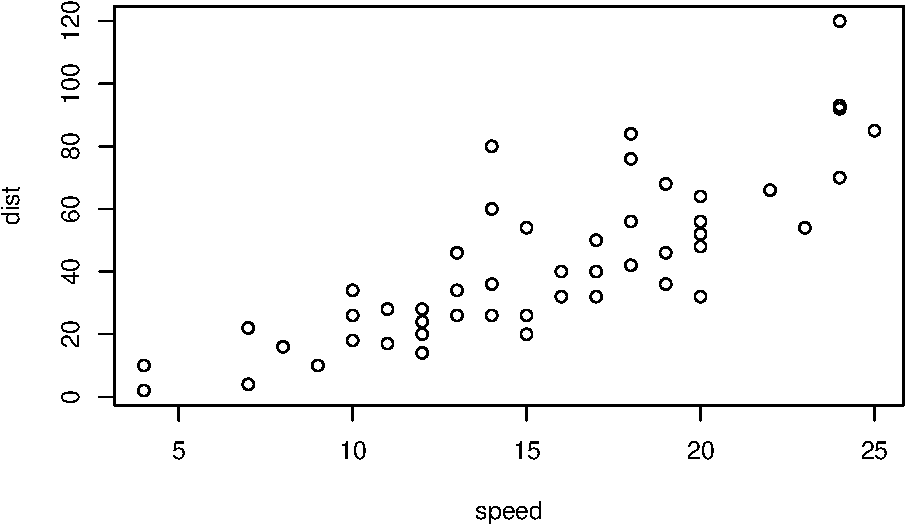
\includegraphics{24-rbasics_files/figure-latex/unnamed-chunk-4-1.pdf}

右下の、窓枠の、Plots に、上のグラフ(散布図)が表示されると思います。Export と書いてある、プルダウンメニューがあり、そこから、画像として保存することも、可能です。

以前は、このように取り出した画像を、Word などに貼り付けて、使っていました。現在でも、そのような方法を知っていることは有効だと思います。

\hypertarget{ux30a2ux30b5ux30a4ux30f3ux30e1ux30f3ux30c8ux30d8ux30ebux30d7}{%
\section{アサインメント、ヘルプ}\label{ux30a2ux30b5ux30a4ux30f3ux30e1ux30f3ux30c8ux30d8ux30ebux30d7}}

コンソールで次のそれぞれを、試してみてください。

\begin{itemize}
\tightlist
\item
  \texttt{df\ \textless{}-\ cars}
\end{itemize}

\texttt{df} に、\texttt{cars} をアサインします。すなわち、\texttt{df} が、\texttt{cars} の内容に置き換わります。\texttt{cars} はデータですが、データを含む、オブジェクトの名前を設定するためにも使います。オブジェクト名は。英文字から始まれば、かなりの自由度がありますが、わたしは、英文字と数字と \texttt{\_}(underscore) 程度しか使わないようにしています。

\begin{itemize}
\tightlist
\item
  \texttt{head(df)}
\end{itemize}

\texttt{head(df)} は、\texttt{head(cars)} と同じ出力が得られます。

\begin{itemize}
\tightlist
\item
  \texttt{View(cars)}
\end{itemize}

左上の、窓枠が開き、\texttt{cars} というデータ の内容が表示されます。列名のところには、三角形も表示され、それを用いると、大きい順、小さい順などに、並び替えることも可能です。また、フィルター機能も使えます。

\begin{itemize}
\tightlist
\item
  \texttt{?cars}
\end{itemize}

右下の、窓枠の Help タブに、\texttt{cars} の情報が表示されます。Help タブにある、虫眼鏡がついた、検索窓(search window)に、\texttt{cars} といれても、同じ結果が得られます。 内容を確認してください。

一番上には \texttt{cars\ \{datasets\}} とありますが、これは、\texttt{datasets} というパッケージの、\texttt{cars} だという意味です。そこで、\texttt{datasets} を調べてみましょう。

\begin{itemize}
\tightlist
\item
  \texttt{?datasets}
\end{itemize}

``The R Datasets Package'' だと書かれていて、さらに、

This package contains a variety of datasets. For a complete list, use library(help = ``datasets'').

さまざまなデータが含まれています。全てのリストをみるには、\texttt{library(help\ =\ "datasets")} を使ってください。

とありますから、\texttt{library(help\ =\ "datasets")} をコンソールに入力してみてください。

\begin{itemize}
\tightlist
\item
  \texttt{library(help\ =\ "datasets")}
\end{itemize}

左上の窓枠に、リストが表示されます。古いデータばかりですが、例として使うには、十分すぎるぐらいの、数のデータがあります。これらは、Toy Data(おもちゃのデータ)と呼ばれることもあります。

\texttt{cars} も見つかりましたか。

\hypertarget{ux304aux3059ux3059ux3081}{%
\section{おすすめ}\label{ux304aux3059ux3059ux3081}}

コンピュータのシステムが、日本語であると、R の言語も日本語になっているはずです。そこで、エラーが発生すると、一部、日本語で表示されます。しかし、ネット上などで、そのエラーの対応を検索するときは、英語のエラーメッセージで検索した方が、解決方法が得られる可能性が圧倒的に高いので、わたしは、英語に設定しています。英語にするには、Console で次のようにします。

言語を英語に設定:\texttt{Sys.setenv(LANG\ =\ "en")}

RStudio を終了して、もう一度起動すると、日本語に戻っていると思います。ですから、作業の最初、または、エラーが出たら、変更することをお勧めします。

日本語に戻したいときは、次のようにします。

言語を日本語に設定:\texttt{Sys.setenv(LANG\ =\ "ja")}

さまざまな Help なども、すべて日本語で表示されれば日本語を使うのは有効かもしれませんが、すくなくとも、現在は、そうではないので、上に説明したことから、英語に設定することをお勧めします。

\hypertarget{ux7df4ux7fd2}{%
\section{練習}\label{ux7df4ux7fd2}}

\begin{enumerate}
\def\labelenumi{\arabic{enumi}.}
\tightlist
\item
  \texttt{head(cars,\ 10L)} は何が出力されますか。\texttt{head(cars,\ n=10L)} と同じですか。
\item
  \texttt{?head} または、Help の検索窓に \texttt{head} と入力して、説明を見てみてください。\texttt{head(cars,\ n=10L)} などについて、書いてありましたか。他には、どのようなことが分かりましたか。
\item
  \texttt{datasets} のデータのいくつかについて、そのデータの help や、\texttt{head}, \texttt{str}, \texttt{summary} などを使ってみてください。これらで表示できない場合はありますか。データについては、最初に、これら、三つを試してみることをお勧めします。わかったことをメモしておくと良いでしょう。\texttt{datasets} のリストをみるには、\texttt{library(help\ =\ "datasets")} でしたね。
\end{enumerate}

\hypertarget{rstudio-ux306bux3064ux3044ux3066}{%
\chapter{RStudio について}\label{rstudio-ux306bux3064ux3044ux3066}}

RStudio は多くの機能を持っています。

\hypertarget{ux56dbux3064ux306eux7a93ux67a0ux3068ux30bfux30d6-four-panes-and-tabs}{%
\section{四つの窓枠とタブ Four Panes and Tabs}\label{ux56dbux3064ux306eux7a93ux67a0ux3068ux30bfux30d6-four-panes-and-tabs}}

\begin{itemize}
\tightlist
\item
  左上(Top Left): スクリプトや文書、データなどの編集(Source Editor)
\item
  右上(Top Right): 環境変数(Environment), 履歴(History) など(etc.)
\item
  左下(Bottom Left): コードの実行・実行結果などを表示するコンソール(Console), コンピュータシステムの端末(Terminal), 文書の機械語翻訳(Render), 背後での作業(Background Jobs)
\item
  右下(Bottom Right): ファイル(Files), 描画(Plots), パッケージ(Packages), ヘルプ(Help), 文書などの表示窓(Viewer), R Markdown の HTML, PDF 表示(Presentation\footnote{Viewerへの表示を使っており、Presentationへの表示を使っておらず不明})
\end{itemize}

\hypertarget{r-script-ux5b9fux884cux8a18ux9332}{%
\chapter{R Script 実行記録}\label{r-script-ux5b9fux884cux8a18ux9332}}

R Script を使って、コードを実行すると、その記録を残すことができます。

\hypertarget{r-script-ux306eux4f5cux6210}{%
\section{R Script の作成}\label{r-script-ux306eux4f5cux6210}}

\begin{itemize}
\tightlist
\item
  RStudio の上のメニュー・バーからFile \textgreater{} New File \textgreater{} R Script を選択します。
\item
  File \textgreater{} Save As で、名前をつけて保存します。\{file\_name\}.R が作成されます。

  \begin{itemize}
  \tightlist
  \item
    右下の、Files から、ファイルを確認してください。
  \end{itemize}
\item
  \texttt{head(cars)}, \texttt{str(cars)}, \texttt{summary(cars)}, \texttt{plot(cars)} などと改行をしながらコードを書きます。
\item
  実行するには、カーソルの場所で Ctrl+Shift+Enter (Win) または Cmd+Shift+Enter (Mac) とすると、カーソルのある行か、その下の行で、最初のコードが実行されます。

  \begin{itemize}
  \tightlist
  \item
    R Script エディターの上にある、Run ボタンを押しても、同様に実行されます。
  \item
    Run ボタンの右の、Source ボタンを押すと、そのスクリプトの、最初からすべてが実行されます。
  \end{itemize}
\item
  最後には保存しておきましょう。たとえば、\texttt{myfirstscript} などとすると、File のところに、\texttt{myfirstscript.R} というファイルができていることを確認できます。
\end{itemize}

\hypertarget{r-script-ux306bux3088ux308bux5b9fux884c}{%
\section{R Script による実行}\label{r-script-ux306bux3088ux308bux5b9fux884c}}

新しく、R Script を作成し、この下の、コード(ハイライトされている部分)をコピー・ペーストして、保存し、実行してみてください。

それぞれ、どのようなことをしているでしょうか。

\hypertarget{ux30b9ux30afux30eaux30d7ux30c81-basics.r}{%
\subsection{\texorpdfstring{スクリプト1: \texttt{basics.R}}{スクリプト1: basics.R}}\label{ux30b9ux30afux30eaux30d7ux30c81-basics.r}}

\begin{Shaded}
\begin{Highlighting}[]
\DocumentationTok{\#\#\#\#\#\#\#\#\#\#\#\#\#\#\#\#\#}
\CommentTok{\#}
\CommentTok{\# basics.R}
\CommentTok{\#}
\DocumentationTok{\#\#\#\#\#\#\#\#\#\#\#\#\#\#\#\#}
\CommentTok{\# \textquotesingle{}Quick R\textquotesingle{} by DataCamp may be a handy reference: }
\CommentTok{\#     https://www.statmethods.net/management/index.html}
\CommentTok{\# Cheat Sheet at RStudio: https://www.rstudio.com/resources/cheatsheets/}
\CommentTok{\# Base R Cheat Sheet: https://github.com/rstudio/cheatsheets/raw/main/base{-}r.pdf}
\CommentTok{\# To execute the line: Control + Enter (Window and Linux), Command + Enter (Mac)}
\DocumentationTok{\#\# try your experiments on the console}

\DocumentationTok{\#\# calculator}

\DecValTok{3} \SpecialCharTok{+} \DecValTok{7}

\DocumentationTok{\#\#\# +, {-}, *, /, \^{} (or **), \%\%, \%/\%}

\DecValTok{3} \SpecialCharTok{+} \DecValTok{10} \SpecialCharTok{/} \DecValTok{2}

\DecValTok{3}\SpecialCharTok{\^{}}\DecValTok{2}

\DecValTok{2}\SpecialCharTok{\^{}}\DecValTok{3}

\DecValTok{2}\SpecialCharTok{*}\DecValTok{2}\SpecialCharTok{*}\DecValTok{2}

\DocumentationTok{\#\#\# assignment: \textless{}{-}, (=, {-}\textgreater{}, assign()) }

\NormalTok{x }\OtherTok{\textless{}{-}} \DecValTok{5}

\NormalTok{x }

\DocumentationTok{\#\#\#\# object\_name \textless{}{-} value, \textquotesingle{}\textless{}{-}\textquotesingle{} shortcut: Alt (option) + \textquotesingle{}{-}\textquotesingle{} (hyphen or minus) }
\DocumentationTok{\#\#\#\# Object names must start with a letter and can only contain letter, numbers, \_ and .}

\NormalTok{this\_is\_a\_long\_name }\OtherTok{\textless{}{-}} \DecValTok{5}\SpecialCharTok{\^{}}\DecValTok{3}

\NormalTok{this\_is\_a\_long\_name}

\NormalTok{char\_name }\OtherTok{\textless{}{-}} \StringTok{"What is your name?"}

\NormalTok{char\_name}

\DocumentationTok{\#\#\#\# Use \textquotesingle{}tab completion\textquotesingle{} and \textquotesingle{}up arrow\textquotesingle{}}

\DocumentationTok{\#\#\# ls(): list of all assignments}

\FunctionTok{ls}\NormalTok{()}
\FunctionTok{ls.str}\NormalTok{()}

\DocumentationTok{\#\#\#\# check Environment in the upper right pane}

\DocumentationTok{\#\#\# (atomic) vectors}

\DecValTok{5}\SpecialCharTok{:}\DecValTok{10}

\NormalTok{a }\OtherTok{\textless{}{-}} \FunctionTok{seq}\NormalTok{(}\DecValTok{5}\NormalTok{,}\DecValTok{10}\NormalTok{)}

\NormalTok{a}

\NormalTok{b }\OtherTok{\textless{}{-}} \DecValTok{5}\SpecialCharTok{:}\DecValTok{10}

\FunctionTok{identical}\NormalTok{(a,b)}

\FunctionTok{seq}\NormalTok{(}\DecValTok{5}\NormalTok{,}\DecValTok{10}\NormalTok{,}\DecValTok{2}\NormalTok{) }\CommentTok{\# same as seq(from = 5, to = 10, by = 2)}

\NormalTok{c1 }\OtherTok{\textless{}{-}} \FunctionTok{seq}\NormalTok{(}\DecValTok{0}\NormalTok{,}\DecValTok{100}\NormalTok{, }\AttributeTok{by =} \DecValTok{10}\NormalTok{)}

\NormalTok{c2 }\OtherTok{\textless{}{-}} \FunctionTok{seq}\NormalTok{(}\DecValTok{0}\NormalTok{,}\DecValTok{100}\NormalTok{, }\AttributeTok{length.out =} \DecValTok{10}\NormalTok{)}

\NormalTok{c1}

\NormalTok{c2}

\FunctionTok{length}\NormalTok{(c1)}

\DocumentationTok{\#\#\#\# ? seq   ? length   ? identical}

\NormalTok{(die }\OtherTok{\textless{}{-}} \DecValTok{1}\SpecialCharTok{:}\DecValTok{6}\NormalTok{)}

\NormalTok{zero\_one }\OtherTok{\textless{}{-}} \FunctionTok{c}\NormalTok{(}\DecValTok{0}\NormalTok{,}\DecValTok{1}\NormalTok{) }\CommentTok{\# same as 0:1}

\NormalTok{die }\SpecialCharTok{+}\NormalTok{ zero\_one }\CommentTok{\# c(1,2,3,4,5,6) + c(0,1). re{-}use}

\NormalTok{d1 }\OtherTok{\textless{}{-}} \FunctionTok{rep}\NormalTok{(}\DecValTok{1}\SpecialCharTok{:}\DecValTok{3}\NormalTok{,}\DecValTok{2}\NormalTok{) }\CommentTok{\# repeat}


\NormalTok{d1}

\NormalTok{die }\SpecialCharTok{==}\NormalTok{ d1}

\NormalTok{d2 }\OtherTok{\textless{}{-}} \FunctionTok{as.character}\NormalTok{(die }\SpecialCharTok{==}\NormalTok{ d1)}

\NormalTok{d2}

\NormalTok{d3 }\OtherTok{\textless{}{-}} \FunctionTok{as.numeric}\NormalTok{(die }\SpecialCharTok{==}\NormalTok{ d1)}

\NormalTok{d3}

\DocumentationTok{\#\#\# class() for class and typeof() for mode}
\DocumentationTok{\#\#\# class of vectors: numeric, charcters, logical}
\DocumentationTok{\#\#\# types of vectors: doubles, integers, characters, logicals (complex and raw)}

\FunctionTok{typeof}\NormalTok{(d1); }\FunctionTok{class}\NormalTok{(d1)}

\FunctionTok{typeof}\NormalTok{(d2); }\FunctionTok{class}\NormalTok{(d2)}

\FunctionTok{typeof}\NormalTok{(d3); }\FunctionTok{class}\NormalTok{(d3)}

\FunctionTok{sqrt}\NormalTok{(}\DecValTok{2}\NormalTok{)}

\FunctionTok{sqrt}\NormalTok{(}\DecValTok{2}\NormalTok{)}\SpecialCharTok{\^{}}\DecValTok{2}

\FunctionTok{sqrt}\NormalTok{(}\DecValTok{2}\NormalTok{)}\SpecialCharTok{\^{}}\DecValTok{2} \SpecialCharTok{{-}} \DecValTok{2}

\FunctionTok{typeof}\NormalTok{(}\FunctionTok{sqrt}\NormalTok{(}\DecValTok{2}\NormalTok{))}

\FunctionTok{typeof}\NormalTok{(}\DecValTok{2}\NormalTok{)}

\FunctionTok{typeof}\NormalTok{(2L)}

\DecValTok{5} \SpecialCharTok{==} \FunctionTok{c}\NormalTok{(}\DecValTok{5}\NormalTok{)}

\FunctionTok{length}\NormalTok{(}\DecValTok{5}\NormalTok{)}

\DocumentationTok{\#\#\# Subsetting}

\NormalTok{(A\_Z }\OtherTok{\textless{}{-}}\NormalTok{ LETTERS)}

\NormalTok{A\_F }\OtherTok{\textless{}{-}}\NormalTok{ A\_Z[}\DecValTok{1}\SpecialCharTok{:}\DecValTok{6}\NormalTok{]}

\NormalTok{A\_F}

\NormalTok{A\_F[}\DecValTok{3}\NormalTok{]}

\NormalTok{A\_F[}\FunctionTok{c}\NormalTok{(}\DecValTok{3}\NormalTok{,}\DecValTok{5}\NormalTok{)]}

\NormalTok{large }\OtherTok{\textless{}{-}}\NormalTok{ die }\SpecialCharTok{\textgreater{}} \DecValTok{3}

\NormalTok{large}

\NormalTok{even }\OtherTok{\textless{}{-}}\NormalTok{ die }\SpecialCharTok{\%in\%} \FunctionTok{c}\NormalTok{(}\DecValTok{2}\NormalTok{,}\DecValTok{4}\NormalTok{,}\DecValTok{6}\NormalTok{)}

\NormalTok{even}

\NormalTok{A\_F[large]}

\NormalTok{A\_F[even]}

\NormalTok{A\_F[die }\SpecialCharTok{\textless{}} \DecValTok{4}\NormalTok{]}

\DocumentationTok{\#\#\# Compare df with df1 \textless{}{-} data.frame(number = die, alphabet = A\_F)}
\NormalTok{df }\OtherTok{\textless{}{-}} \FunctionTok{data.frame}\NormalTok{(}\AttributeTok{number =}\NormalTok{ die, }\AttributeTok{alphabet =}\NormalTok{ A\_F, }\AttributeTok{stringsAsFactors =} \ConstantTok{FALSE}\NormalTok{)}

\NormalTok{df}

\NormalTok{df}\SpecialCharTok{$}\NormalTok{number}

\NormalTok{df}\SpecialCharTok{$}\NormalTok{alphabet}

\NormalTok{df[}\DecValTok{3}\NormalTok{,}\DecValTok{2}\NormalTok{]}

\NormalTok{df[}\DecValTok{4}\NormalTok{,}\DecValTok{1}\NormalTok{]}

\NormalTok{df[}\DecValTok{1}\NormalTok{]}

\FunctionTok{class}\NormalTok{(df[}\DecValTok{1}\NormalTok{])}

\FunctionTok{class}\NormalTok{(df[[}\DecValTok{1}\NormalTok{]])}

\FunctionTok{identical}\NormalTok{(df[[}\DecValTok{1}\NormalTok{]], die)}

\FunctionTok{identical}\NormalTok{(df[}\DecValTok{1}\NormalTok{],die)}

\DocumentationTok{\#\#\#\#\#\#\#\#\#\#\#\#\#\#\#\#\#\#\#\#}
\CommentTok{\# The First Example}
\DocumentationTok{\#\#\#\#\#\#\#\#\#\#\#\#\#\#\#\#\#\#\#\#}

\FunctionTok{plot}\NormalTok{(cars)}

\CommentTok{\# Help}

\NormalTok{? cars}

\CommentTok{\# cars is in the \textquotesingle{}datasets\textquotesingle{} package}

\FunctionTok{data}\NormalTok{()}

\CommentTok{\# help(cars) does the same as ? cars}
\CommentTok{\# You can use Help tab in the right bottom pane}

\FunctionTok{help}\NormalTok{(plot)}
\NormalTok{? par}

\FunctionTok{head}\NormalTok{(cars)}

\FunctionTok{str}\NormalTok{(cars)}

\FunctionTok{summary}\NormalTok{(cars)}

\NormalTok{x }\OtherTok{\textless{}{-}}\NormalTok{ cars}\SpecialCharTok{$}\NormalTok{speed}
\NormalTok{y }\OtherTok{\textless{}{-}}\NormalTok{ cars}\SpecialCharTok{$}\NormalTok{dist}

\FunctionTok{min}\NormalTok{(x)}
\FunctionTok{mean}\NormalTok{(x)}
\FunctionTok{quantile}\NormalTok{(x)}

\FunctionTok{plot}\NormalTok{(cars)}

\FunctionTok{abline}\NormalTok{(}\FunctionTok{lm}\NormalTok{(cars}\SpecialCharTok{$}\NormalTok{dist }\SpecialCharTok{\textasciitilde{}}\NormalTok{ cars}\SpecialCharTok{$}\NormalTok{speed))}

\FunctionTok{summary}\NormalTok{(}\FunctionTok{lm}\NormalTok{(cars}\SpecialCharTok{$}\NormalTok{dist }\SpecialCharTok{\textasciitilde{}}\NormalTok{ cars}\SpecialCharTok{$}\NormalTok{speed))}

\FunctionTok{boxplot}\NormalTok{(cars)}

\FunctionTok{hist}\NormalTok{(cars}\SpecialCharTok{$}\NormalTok{speed)}
\FunctionTok{hist}\NormalTok{(cars}\SpecialCharTok{$}\NormalTok{dist)}
\FunctionTok{hist}\NormalTok{(cars}\SpecialCharTok{$}\NormalTok{dist, }\AttributeTok{breaks =} \FunctionTok{seq}\NormalTok{(}\DecValTok{0}\NormalTok{,}\DecValTok{120}\NormalTok{, }\DecValTok{10}\NormalTok{))}
\end{Highlighting}
\end{Shaded}

\hypertarget{ux30b9ux30afux30eaux30d7ux30c82-coronavirus.r}{%
\subsection{\texorpdfstring{スクリプト2: \texttt{coronavirus.R}}{スクリプト2: coronavirus.R}}\label{ux30b9ux30afux30eaux30d7ux30c82-coronavirus.r}}

\begin{Shaded}
\begin{Highlighting}[]
\CommentTok{\# https://coronavirus.jhu.edu/map.html}
\CommentTok{\# JHU Covid{-}19 global time series data}
\CommentTok{\# See R package coronavirus at: https://github.com/RamiKrispin/coronavirus}
\CommentTok{\# Data taken from: https://github.com/RamiKrispin/coronavirus/tree/master/csv}
\CommentTok{\# Last Updated}
\FunctionTok{Sys.Date}\NormalTok{()}

\DocumentationTok{\#\# Download and read csv (comma separated value) file}
\NormalTok{coronavirus }\OtherTok{\textless{}{-}} \FunctionTok{read.csv}\NormalTok{(}\StringTok{"https://github.com/RamiKrispin/coronavirus/raw/master/csv/coronavirus.csv"}\NormalTok{)}
\CommentTok{\# write.csv(coronavirus, "data/coronavirus.csv")}

\DocumentationTok{\#\# Summaries and structures of the data}
\FunctionTok{head}\NormalTok{(coronavirus)}
\FunctionTok{str}\NormalTok{(coronavirus)}
\NormalTok{coronavirus}\SpecialCharTok{$}\NormalTok{date }\OtherTok{\textless{}{-}} \FunctionTok{as.Date}\NormalTok{(coronavirus}\SpecialCharTok{$}\NormalTok{date)}
\FunctionTok{str}\NormalTok{(coronavirus)}

\FunctionTok{range}\NormalTok{(coronavirus}\SpecialCharTok{$}\NormalTok{date)}
\FunctionTok{unique}\NormalTok{(coronavirus}\SpecialCharTok{$}\NormalTok{country)}
\FunctionTok{unique}\NormalTok{(coronavirus}\SpecialCharTok{$}\NormalTok{type)}

\DocumentationTok{\#\# Set Country}
\NormalTok{COUNTRY }\OtherTok{\textless{}{-}} \StringTok{"Japan"}
\NormalTok{df0 }\OtherTok{\textless{}{-}}\NormalTok{ coronavirus[coronavirus}\SpecialCharTok{$}\NormalTok{country }\SpecialCharTok{==}\NormalTok{ COUNTRY,]}
\FunctionTok{head}\NormalTok{(df0)}
\FunctionTok{tail}\NormalTok{(df0)}
\NormalTok{(pop }\OtherTok{\textless{}{-}}\NormalTok{ df0}\SpecialCharTok{$}\NormalTok{population[}\DecValTok{1}\NormalTok{])}
\NormalTok{df }\OtherTok{\textless{}{-}}\NormalTok{ df0[}\FunctionTok{c}\NormalTok{(}\DecValTok{1}\NormalTok{,}\DecValTok{6}\NormalTok{,}\DecValTok{7}\NormalTok{,}\DecValTok{13}\NormalTok{)]}
\FunctionTok{str}\NormalTok{(df)}
\FunctionTok{head}\NormalTok{(df)}
\DocumentationTok{\#\#\# alternatively,}
\FunctionTok{head}\NormalTok{(df0[}\FunctionTok{c}\NormalTok{(}\StringTok{"date"}\NormalTok{, }\StringTok{"type"}\NormalTok{, }\StringTok{"cases"}\NormalTok{, }\StringTok{"population"}\NormalTok{)])}
\DocumentationTok{\#\#\#}

\DocumentationTok{\#\# Set types}
\NormalTok{df\_confirmed }\OtherTok{\textless{}{-}}\NormalTok{ df[df}\SpecialCharTok{$}\NormalTok{type }\SpecialCharTok{==} \StringTok{"confirmed"}\NormalTok{,]}
\NormalTok{df\_death }\OtherTok{\textless{}{-}}\NormalTok{ df[df}\SpecialCharTok{$}\NormalTok{type }\SpecialCharTok{==} \StringTok{"death"}\NormalTok{,]}
\NormalTok{df\_recovery }\OtherTok{\textless{}{-}}\NormalTok{ df[df}\SpecialCharTok{$}\NormalTok{data\_type }\SpecialCharTok{==} \StringTok{"recovery"}\NormalTok{,]}
\FunctionTok{head}\NormalTok{(df\_confirmed)}
\FunctionTok{head}\NormalTok{(df\_death)}
\FunctionTok{head}\NormalTok{(df\_recovery)}

\DocumentationTok{\#\# Histogram}
\FunctionTok{plot}\NormalTok{(df\_confirmed}\SpecialCharTok{$}\NormalTok{date, df\_confirmed}\SpecialCharTok{$}\NormalTok{cases, }\AttributeTok{type =} \StringTok{"h"}\NormalTok{)}
\FunctionTok{plot}\NormalTok{(df\_death}\SpecialCharTok{$}\NormalTok{date, df\_death}\SpecialCharTok{$}\NormalTok{cases, }\AttributeTok{type =} \StringTok{"h"}\NormalTok{)}
\CommentTok{\# plot(df\_recovered$date, df\_recovered$cases, type = "h") \# no data for recovery}

\DocumentationTok{\#\# Scatter plot and correlation}
\FunctionTok{plot}\NormalTok{(df\_confirmed}\SpecialCharTok{$}\NormalTok{cases, df\_death}\SpecialCharTok{$}\NormalTok{cases, }\AttributeTok{type =} \StringTok{"p"}\NormalTok{)}
\FunctionTok{cor}\NormalTok{(df\_confirmed}\SpecialCharTok{$}\NormalTok{cases, df\_death}\SpecialCharTok{$}\NormalTok{cases)}


\DocumentationTok{\#\# In addition set a period}
\NormalTok{start\_date }\OtherTok{\textless{}{-}} \FunctionTok{as.Date}\NormalTok{(}\StringTok{"2022{-}07{-}01"}\NormalTok{)}
\NormalTok{end\_date }\OtherTok{\textless{}{-}} \FunctionTok{Sys.Date}\NormalTok{() }
\NormalTok{df\_date }\OtherTok{\textless{}{-}}\NormalTok{ df[df}\SpecialCharTok{$}\NormalTok{date }\SpecialCharTok{\textgreater{}=}\NormalTok{start\_date }\SpecialCharTok{\&}\NormalTok{ df}\SpecialCharTok{$}\NormalTok{date }\SpecialCharTok{\textless{}=}\NormalTok{ end\_date,]}
\DocumentationTok{\#\#}

\DocumentationTok{\#\# Set types}
\NormalTok{df\_date\_confirmed }\OtherTok{\textless{}{-}}\NormalTok{ df\_date[df\_date}\SpecialCharTok{$}\NormalTok{type }\SpecialCharTok{==} \StringTok{"confirmed"}\NormalTok{,]}
\NormalTok{df\_date\_death }\OtherTok{\textless{}{-}}\NormalTok{ df\_date[df\_date}\SpecialCharTok{$}\NormalTok{type }\SpecialCharTok{==} \StringTok{"death"}\NormalTok{,]}
\NormalTok{df\_date\_recovery }\OtherTok{\textless{}{-}}\NormalTok{ df\_date[df\_date}\SpecialCharTok{$}\NormalTok{data\_type }\SpecialCharTok{==} \StringTok{"recovery"}\NormalTok{,]}
\FunctionTok{head}\NormalTok{(df\_date\_confirmed)}
\FunctionTok{head}\NormalTok{(df\_date\_death)}
\FunctionTok{head}\NormalTok{(df\_date\_recovery)}

\DocumentationTok{\#\# Histogram}
\FunctionTok{plot}\NormalTok{(df\_date\_confirmed}\SpecialCharTok{$}\NormalTok{date, df\_date\_confirmed}\SpecialCharTok{$}\NormalTok{cases, }\AttributeTok{type =} \StringTok{"h"}\NormalTok{)}
\FunctionTok{plot}\NormalTok{(df\_date\_death}\SpecialCharTok{$}\NormalTok{date, df\_date\_death}\SpecialCharTok{$}\NormalTok{cases, }\AttributeTok{type =} \StringTok{"h"}\NormalTok{)}
\CommentTok{\# plot(df\_date\_recovered$date, df\_date\_recovered$cases, type = "h") \# no data for recovery}

\FunctionTok{plot}\NormalTok{(df\_date\_confirmed}\SpecialCharTok{$}\NormalTok{cases, df\_date\_death}\SpecialCharTok{$}\NormalTok{cases, }\AttributeTok{type =} \StringTok{"p"}\NormalTok{)}
\FunctionTok{cor}\NormalTok{(df\_date\_confirmed}\SpecialCharTok{$}\NormalTok{cases, df\_date\_death}\SpecialCharTok{$}\NormalTok{cases)}

\DocumentationTok{\#\#\#\# Extra}
\FunctionTok{plot}\NormalTok{(df\_confirmed}\SpecialCharTok{$}\NormalTok{date, df\_confirmed}\SpecialCharTok{$}\NormalTok{cases, }\AttributeTok{type =} \StringTok{"h"}\NormalTok{, }
     \AttributeTok{main =} \FunctionTok{paste}\NormalTok{(}\StringTok{"Comfirmed Cases in"}\NormalTok{,COUNTRY), }
     \AttributeTok{xlab =} \StringTok{"Date"}\NormalTok{, }\AttributeTok{ylab =} \StringTok{"Number of Cases"}\NormalTok{)}
\end{Highlighting}
\end{Shaded}

\hypertarget{ux7df4ux7fd2-1}{%
\section{練習}\label{ux7df4ux7fd2-1}}

上の、\texttt{coronavirus.R} について

\begin{enumerate}
\def\labelenumi{\arabic{enumi}.}
\tightlist
\item
  \texttt{COUNTRY\ \textless{}-\ "Japan"} の Japan を他の国に変えてみましょう。
\item
  \texttt{start\_date\ \textless{}-\ as.Date("2022-07-01")} の日付を、他の日付に変えてみましょう。
\item
  \texttt{df\_confirmed\$cases} と \texttt{df\_death\$cases} についてどんなことがわかりますか。
\item
  発見や、問いがあれば、書き出してみましょう。
\end{enumerate}

\hypertarget{tips}{%
\section{Tips}\label{tips}}

キーボード・ショートカットと言われる、さまざまな機能があります。

\begin{itemize}
\tightlist
\item
  上のメニュー・バー: Help \textgreater{} Keyboard Short Cut Help 確認してみてください。
\item
  右下の窓枠: Files タブから、ファイルの確認ができます。
\end{itemize}

\hypertarget{ux30d1ux30c3ux30b1ux30fcux30b8---packages}{%
\chapter{パッケージ - Packages}\label{ux30d1ux30c3ux30b1ux30fcux30b8---packages}}

\begin{quote}
R packages are extensions to the R statistical programming language containing code, data, and documentation in a standardised collection format that can be installed by users of R using Tool \textgreater{} Install Packages in the top menu bar of R Studio. \url{https://en.wikipedia.org/wiki/R_package}
\end{quote}

\begin{quote}
Rパッケージは、Rの拡張機能で、コード、データ、ドキュメントを標準化されたコレクション形式で含んでおり、標準的なものは、R Studio の Top Bar の Tool \textgreater{} Install Packages からインストールできます。
\end{quote}

\hypertarget{ux30d1ux30c3ux30b1ux30fcux30b8ux306eux30a4ux30f3ux30b9ux30c8ux30fcux30eb}{%
\section{パッケージのインストール}\label{ux30d1ux30c3ux30b1ux30fcux30b8ux306eux30a4ux30f3ux30b9ux30c8ux30fcux30eb}}

いずれ使いますので、まずは、三つのパッケージをインストールしてみましょう。

\begin{itemize}
\tightlist
\item
  \texttt{tidyverse}
\item
  \texttt{rmarkdown}
\item
  \texttt{tinytex}
\end{itemize}

インストール方法はいくつかあります。

一つ目は、上のメニューバーの Tool から、Install Packages \ldots{} を選択します。そして、パッケージーズにインストールしたい、パッケージ名を入力します。そのパッケージ名が下にも出れば、Install ボタンを押してください。入力した名前の下にパッケージ名が出ない場合は、スペルが間違っている可能性がありますから、確認して、入れ直してください。

Console に、\texttt{install.packages("tidyverse")} などと表示され、たくさんメッセージが出ます。終了すると、\textgreater{} のマークがでます。

二つ目は、\texttt{install.packages("tidyverse")} のような書式で書いて、Console に入れる方法です。

三つ目は、右下の窓枠の Packages のタブにある、Install というボタンを押す方法です。すると、一番目の方法に、戻り、パッケージ名を入力できるようになります。

この Packages タブにある、ものが、すでに、インストールされているパッケージです。そのなかで、\texttt{base} や、\texttt{datasets} などいくつかに、チェックがついていると思いますが、それらは、ロードされていて、いつでも、使える状態になっていることを意味しています。ロードは、たとえば、\texttt{library(tidyverse)} のようにしますが、それは、いずれもう一度説明します。

インストールは一回だけ。ときどき、Tools \textgreater{} Check for Package Update をつかって、Update しておくと良いでしょう。

パッケージのインストールで問題が生じることがあります。特に、Windows の日本語システムの場合です。(4.3.2 R Studio の インストール の下に書いてある部分を参照してください。)

回避方法もいくつかあるようですが、混乱をさけるため、その場合は、Posit Cloud(旧:RStudio Cloud)を使うと良いでしょう。それを見越して、最初は、Posit Cloud ではじめることを、わたしはお薦めしています。自分のコンピュータで、R が RStudio 上で問題なく動いていても、Cloud 上にアカウントを持っていて、実行できることは有効ですし、全員が、同じ環境で作業できることもたいせつなことです。他にも、すぐ、Cheat Sheets(早見表)や、Posit Primers という練習問題(Tutorial)を利用できたり、プロジェクトを共有したりなど、さまざまなメリットがあります。

\hypertarget{ux5099ux8003}{%
\section{備考}\label{ux5099ux8003}}

Package によっては、Source から Compile するかと聞いてくる場合があります。どちらでも、良いのですが、特に、問題が起こっていなければ、No でよいと思います。コンピュータにあった形でインストールすることが必要な場合は、Yes とします。

同じパッケージをもう一度、インストールしたり、または、関連するパッケージがあるような場合、R をリスタートするかと聞いてくることがあります。特に問題が起こらなければ、No で構いません。ただ、エラーが起こって、それに関連して、特別なパッケージをインストールする必要がある場合がありますが、そのときは、Yes としてください。

\hypertarget{ux7df4ux7fd2ux554fux984c-posit-primers}{%
\chapter{練習問題 Posit Primers}\label{ux7df4ux7fd2ux554fux984c-posit-primers}}

Posit Primers \url{https://posit.cloud/learn/primers}

教科書 \href{https://r4ds.had.co.nz}{``R for Data Science''} は、\texttt{tidyverse} パッケージを中心に、データサイエンスについて解説したものですが、Posit Primers は、演習問題をしながら、教科書の内容を理解できるように構成されています。

Posit Cloud からは、左のメニュー(隠れている場合は左上の3本線をクリックして表示させて)から選ぶことができます。そうでない場合は、直接、上のリンクから、利用してください。

\hypertarget{ux6700ux521dux306eux6f14ux7fd2-the-basics-r4ds-explore-i}{%
\section{最初の演習 The Basics -- r4ds: Explore, I}\label{ux6700ux521dux306eux6f14ux7fd2-the-basics-r4ds-explore-i}}

\begin{itemize}
\tightlist
\item
  \href{https://rstudio.cloud/learn/primers/1.1}{Visualization Basics}
\item
  \href{https://rstudio.cloud/learn/primers/1.2}{Programming Basics}
\end{itemize}

ぜひこれら二つの演習問題を、トライしてください。解説を読んでいただけでは、データサイエンスは身につきません。

\hypertarget{ux53c2ux8003ux6587ux732e-references}{%
\chapter{参考文献 References}\label{ux53c2ux8003ux6587ux732e-references}}

一番目は、すでに紹介した、教科書です。二番目は、この文書を作成している、Bookdown というパッケージのサイトですが、そこに、たくさんの本が、無償で公開されています。素晴らしい本がたくさん含まれています。

\begin{itemize}
\tightlist
\item
  R For Data Science, by H. Wickham: \url{https://r4ds.had.co.nz}

  \begin{itemize}
  \tightlist
  \item
    Introduction: \url{https://r4ds.had.co.nz/explore-intro.html\#explore-intro}
  \end{itemize}
\item
  Bookdown: \url{https://bookdown.org}, \href{https://bookdown.org/home/archive/}{Archive}
\end{itemize}

下の一番目は、R 入門を、2時限の講義でしたときのものです。二番目と三番目は、講義で使ったものを、まとめたものです。教科書のようには、できていませんが、参考になる部分もあるかと思いますので、紹介しておきます。

\begin{itemize}
\tightlist
\item
  \href{https://ds-sl.github.io/intro2r/intro2r.nb.html}{Introducton to R}
\item
  \href{https://icu-hsuzuki.github.io/da4r2022/}{Data Analysis for Researchers 2022}
\item
  \href{https://icu-hsuzuki.github.io/da4r2021/}{Data Analysis for Researchers 2021}
\end{itemize}

\hypertarget{youtube-video---getstarted}{%
\chapter{YouTube Video - getstarted}\label{youtube-video---getstarted}}

\begin{itemize}
\tightlist
\item
  ファイル:\url{https://ds-sl.github.io/intro2r/getstarted.html}
\end{itemize}

\hypertarget{part-part-iii-institutional-data}{%
\part*{(PART) PART III INSTITUTIONAL DATA}\label{part-part-iii-institutional-data}}
\addcontentsline{toc}{part}{(PART) PART III INSTITUTIONAL DATA}

\hypertarget{worldbank}{%
\part{World Bank}\label{worldbank}}

\hypertarget{world-development-indicator-wdi}{%
\chapter{World Development Indicator (WDI)}\label{world-development-indicator-wdi}}

パッケージ と \texttt{tidyverse} と \texttt{WDI} を使いますから、下のコードによって、ロードします。

\begin{Shaded}
\begin{Highlighting}[]
\FunctionTok{library}\NormalTok{(tidyverse)}
\CommentTok{\#\textgreater{} {-}{-} Attaching packages {-}{-}{-}{-}{-}{-}{-}{-}{-}{-}{-}{-}{-}{-}{-}{-}{-}{-}{-} tidyverse 1.3.2 {-}{-}}
\CommentTok{\#\textgreater{} v ggplot2 3.4.1     v purrr   1.0.1}
\CommentTok{\#\textgreater{} v tibble  3.1.8     v dplyr   1.1.0}
\CommentTok{\#\textgreater{} v tidyr   1.3.0     v stringr 1.5.0}
\CommentTok{\#\textgreater{} v readr   2.1.4     v forcats 1.0.0}
\CommentTok{\#\textgreater{} {-}{-} Conflicts {-}{-}{-}{-}{-}{-}{-}{-}{-}{-}{-}{-}{-}{-}{-}{-}{-}{-}{-}{-}{-}{-} tidyverse\_conflicts() {-}{-}}
\CommentTok{\#\textgreater{} x dplyr::filter() masks stats::filter()}
\CommentTok{\#\textgreater{} x dplyr::lag()    masks stats::lag()}
\FunctionTok{library}\NormalTok{(WDI)}
\end{Highlighting}
\end{Shaded}

まず、三つの例を見てみましょう。なにをしているかわかりますか。考えて見てください。

\begin{Shaded}
\begin{Highlighting}[]
\FunctionTok{WDI}\NormalTok{(}\AttributeTok{country =} \StringTok{"all"}\NormalTok{, }\AttributeTok{indicator =} \FunctionTok{c}\NormalTok{(}\AttributeTok{gdp =} \StringTok{"NY.GDP.MKTP.CD"}\NormalTok{),}
    \AttributeTok{extra=}\ConstantTok{TRUE}\NormalTok{) }\SpecialCharTok{\%\textgreater{}\%} \FunctionTok{drop\_na}\NormalTok{(gdp) }\SpecialCharTok{\%\textgreater{}\%}
  \FunctionTok{filter}\NormalTok{(year}\SpecialCharTok{==}\FunctionTok{max}\NormalTok{(year), income }\SpecialCharTok{!=}\StringTok{"Aggregates"}\NormalTok{) }\SpecialCharTok{\%\textgreater{}\%} 
  \FunctionTok{drop\_na}\NormalTok{(region) }\SpecialCharTok{\%\textgreater{}\%} \FunctionTok{arrange}\NormalTok{(}\FunctionTok{desc}\NormalTok{(gdp))}
\end{Highlighting}
\end{Shaded}

\begin{verbatim}
#> Rows: 16492 Columns: 13
#> -- Column specification ------------------------------------
#> Delimiter: ","
#> chr  (7): country, iso2c, iso3c, region, capital, income...
#> dbl  (4): year, gdp, longitude, latitude
#> lgl  (1): status
#> date (1): lastupdated
#> 
#> i Use `spec()` to retrieve the full column specification for this data.
#> i Specify the column types or set `show_col_types = FALSE` to quiet this message.
#> # A tibble: 196 x 13
#>    country       iso2c iso3c  year     gdp status lastupda~1
#>    <chr>         <chr> <chr> <dbl>   <dbl> <lgl>  <date>    
#>  1 United States US    USA    2021 2.33e13 NA     2022-12-22
#>  2 China         CN    CHN    2021 1.77e13 NA     2022-12-22
#>  3 Japan         JP    JPN    2021 4.94e12 NA     2022-12-22
#>  4 Germany       DE    DEU    2021 4.26e12 NA     2022-12-22
#>  5 India         IN    IND    2021 3.18e12 NA     2022-12-22
#>  6 United Kingd~ GB    GBR    2021 3.13e12 NA     2022-12-22
#>  7 France        FR    FRA    2021 2.96e12 NA     2022-12-22
#>  8 Italy         IT    ITA    2021 2.11e12 NA     2022-12-22
#>  9 Canada        CA    CAN    2021 1.99e12 NA     2022-12-22
#> 10 Korea, Rep.   KR    KOR    2021 1.81e12 NA     2022-12-22
#> # ... with 186 more rows, 6 more variables: region <chr>,
#> #   capital <chr>, longitude <dbl>, latitude <dbl>,
#> #   income <chr>, lending <chr>, and abbreviated variable
#> #   name 1: lastupdated
\end{verbatim}

\begin{Shaded}
\begin{Highlighting}[]
\FunctionTok{WDI}\NormalTok{(}\AttributeTok{country =} \FunctionTok{c}\NormalTok{(}\StringTok{"CN"}\NormalTok{,}\StringTok{"GB"}\NormalTok{,}\StringTok{"JP"}\NormalTok{,}\StringTok{"IN"}\NormalTok{,}\StringTok{"US"}\NormalTok{,}\StringTok{"DE"}\NormalTok{), }\AttributeTok{indicator =} \FunctionTok{c}\NormalTok{(}\AttributeTok{gdp =} \StringTok{"NY.GDP.MKTP.CD"}\NormalTok{), }\AttributeTok{extra=}\ConstantTok{TRUE}\NormalTok{) }\SpecialCharTok{\%\textgreater{}\%} \FunctionTok{drop\_na}\NormalTok{(gdp) }\SpecialCharTok{\%\textgreater{}\%} 
  \FunctionTok{ggplot}\NormalTok{(}\FunctionTok{aes}\NormalTok{(year, gdp, }\AttributeTok{col =}\NormalTok{ country)) }\SpecialCharTok{+} \FunctionTok{geom\_line}\NormalTok{() }\SpecialCharTok{+}
  \FunctionTok{labs}\NormalTok{(}\AttributeTok{title =} \StringTok{"WDI NY.GDP.MKTP.CD: gdp"}\NormalTok{)}
\end{Highlighting}
\end{Shaded}

\begin{verbatim}
#> Rows: 372 Columns: 13
#> -- Column specification ------------------------------------
#> Delimiter: ","
#> chr  (7): country, iso2c, iso3c, region, capital, income...
#> dbl  (4): year, gdp, longitude, latitude
#> lgl  (1): status
#> date (1): lastupdated
#> 
#> i Use `spec()` to retrieve the full column specification for this data.
#> i Specify the column types or set `show_col_types = FALSE` to quiet this message.
\end{verbatim}

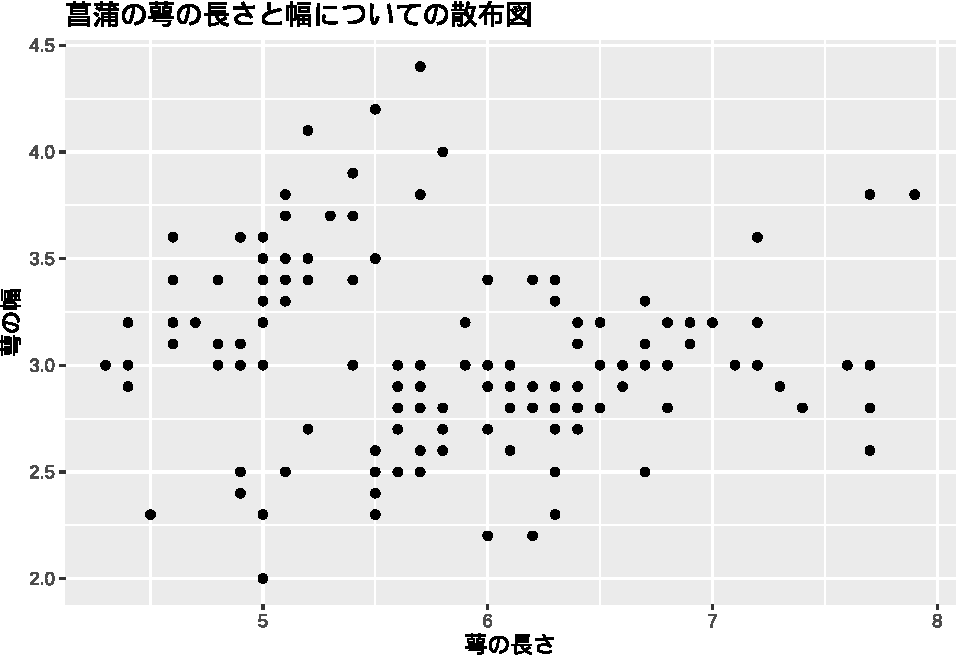
\includegraphics{31-worldbank_files/figure-latex/unnamed-chunk-8-1.pdf}

\begin{Shaded}
\begin{Highlighting}[]
\FunctionTok{WDI}\NormalTok{(}\AttributeTok{country =} \FunctionTok{c}\NormalTok{(}\StringTok{"CN"}\NormalTok{,}\StringTok{"IN"}\NormalTok{,}\StringTok{"JP"}\NormalTok{,}\StringTok{"US"}\NormalTok{), }
    \AttributeTok{indicator =} \FunctionTok{c}\NormalTok{(}\AttributeTok{gdp\_growth\_rate =} \StringTok{"NY.GDP.MKTP.KD.ZG"}\NormalTok{), }\AttributeTok{extra=}\ConstantTok{TRUE}\NormalTok{) }\SpecialCharTok{\%\textgreater{}\%}
  \FunctionTok{drop\_na}\NormalTok{(gdp\_growth\_rate) }\SpecialCharTok{\%\textgreater{}\%} 
  \FunctionTok{ggplot}\NormalTok{(}\FunctionTok{aes}\NormalTok{(year, gdp\_growth\_rate, }\AttributeTok{col =}\NormalTok{ country)) }\SpecialCharTok{+} \FunctionTok{geom\_line}\NormalTok{() }\SpecialCharTok{+}
  \FunctionTok{labs}\NormalTok{(}\AttributeTok{title =} \FunctionTok{paste}\NormalTok{(}\StringTok{"WDI NY.GDP.MKTP.KD.ZG: gdp growth rate"}\NormalTok{))}
\end{Highlighting}
\end{Shaded}

\begin{verbatim}
#> Rows: 248 Columns: 13
#> -- Column specification ------------------------------------
#> Delimiter: ","
#> chr  (7): country, iso2c, iso3c, region, capital, income...
#> dbl  (4): year, gdp_growth_rate, longitude, latitude
#> lgl  (1): status
#> date (1): lastupdated
#> 
#> i Use `spec()` to retrieve the full column specification for this data.
#> i Specify the column types or set `show_col_types = FALSE` to quiet this message.
\end{verbatim}

\includegraphics{31-worldbank_files/figure-latex/unnamed-chunk-11-1.pdf}

まず、世界の国々の、GDP(gross domestic product 国内総生産)のデータを、取得して、2021年の GDP を大きな順に並べています。

値は、たとえば、\(2.331508e+13\) のように書かれていますが、これは、科学的記法と呼ばれるもので、\(2.331508 \times 10^{13}\) を意味しています。約23兆ドルです。

次に、3兆ドル以上の、6カ国を選択し、その、iso2c と呼ばれるコードを使って、それらの国のデータをもう一度取得し、年次変化をあらわすグラフを描いています。

さらにその中から、4カ国を選んで、今度は、GDP の年次変化率を描いています。単位は、パーセントです。

これは、ひとつの例ですが、ここで使われているのが、WDI World Development Indicator というもので、世界銀行が、いくつかの指標を定めて、編纂しているものです。

\hypertarget{ux6307ux6a19-indicators-wdi}{%
\section{指標 Indicators (WDI)}\label{ux6307ux6a19-indicators-wdi}}

上の例では、次の二つの指標のコード Indicator Code (WDI Code) が使われました。

\begin{itemize}
\tightlist
\item
  NY.GDP.MKTP.CD: GDP (current US\$)
\item
  NY.GDP.MKTP.KD.ZG: GDP growth (annual \%)
\end{itemize}

\hypertarget{ux6307ux6a19-wdi-world-development-indicators}{%
\section{指標 WDI (World Development Indicators)}\label{ux6307ux6a19-wdi-world-development-indicators}}

\begin{quote}
The World Development Indicators is a compilation of relevant, high-quality, and internationally comparable statistics about global development and the fight against poverty. The database contains 1,400 time series indicators for 217 economies and more than 40 country groups, with data for many indicators going back more than 50 years.
\end{quote}

\begin{quote}
WDIは、世界の開発状況と、貧困との戦いに関する、適切で上質、かつ、国際的に比較可能な時系列の統計データを編纂したものです。このデータベースは、217の経済と40以上の国グループについて1,400の時系列指標を含み、指標のデータの多くは50年以上前に遡ることができます。
\end{quote}

\begin{itemize}
\tightlist
\item
  世界銀行(World Bank): \url{https://www.worldbank.org}
\item
  World Bank Open Data: \url{https://data.worldbank.org}

  \begin{itemize}
  \tightlist
  \item
    Country / Indicator \textgreater{} Featured \& All \textgreater{} Details
  \end{itemize}
\item
  \href{https://datatopics.worldbank.org/world-development-indicators/}{World Development Indicators (WDI)} :

  \begin{itemize}
  \tightlist
  \item
    Themes: Poverty and Inequality, People, Environment, Economy, States and Markets, Global Links
  \item
    Open Data \& DataBank: Explore data, Query database
  \end{itemize}
\end{itemize}

\hypertarget{ux6307ux6a19-ux306eux30b3ux30fcux30c9wdi-code-ux3092ux63a2ux3057ux3066ux307fux3088ux3046}{%
\section{指標 のコード、WDI code を探してみよう}\label{ux6307ux6a19-ux306eux30b3ux30fcux30c9wdi-code-ux3092ux63a2ux3057ux3066ux307fux3088ux3046}}

いくつかの探し方があります。まず、ここでは、World Bank のサイトから探す方法を説明しましょう。

ふた通りあります。

\begin{enumerate}
\def\labelenumi{\arabic{enumi}.}
\item
  \href{https://data.worldbank.org}{World Bank Open Data} にいくと、表題の下の検索窓の下に、 Country / Indicator とありますから、Indicator を選択します。すると、そこに、項目のリストが、Featured と All という二つのタブに分かれて出ています。かなり膨大です。それを選択すると、その項目のサイトに行きます。それが、指標のサイトです。図などの、右上に、Details とありますから、それを選択すると、その中に、Indicator が書かれています。 実は、指標のサイトのアドレス(URL)を見ると、そこにも、この Indicator が書かれていることがわかります。
\item
  \href{https://datatopics.worldbank.org/world-development-indicators/}{World Development Indicators (WDI)} にいくと、下のようなテーマに分かれています。
\end{enumerate}

Themes: Poverty and Inequality, People, Environment, Economy, States and Markets, Global Links

その中から、選択して、スクロールすると、そこに、指標が書かれています。

Indicator, Code, Time coverage, Region coverage, Get data

とあり、Code が、指標のコードです。実は、すべての年や、すべての地域のデータが揃っているわけではないので、この情報を見ておくことはとても重要です。ほとんど、データがない場合もあります。

一番右端の Get data からは、CSV や、データバンク(Data Bank)へのリンクがあります。

それぞれの方法で、上で使った、二つの指標およびそのコードは見つかりましたか。

1 の方法の途中に出てきた、検索窓から検索することも可能です。

\hypertarget{ux6307ux6a19-wdiux306eux4f8b}{%
\section{指標 WDIの例}\label{ux6307ux6a19-wdiux306eux4f8b}}

このあとの、例で使う指標を書いておきます。

\begin{itemize}
\tightlist
\item
  NY.GDP.MKTP.CD: GDP (current US\$)
\item
  NY.GDP.DEFL.KD.ZG: Inflation, GDP deflator (annual \%)
\item
  SL.UEM.TOTL.NE.ZS: Unemployment, total (\% of total labor force) (national estimate)
\item
  CPTOTNSXN: CPI Price, nominal
\item
  SL.TLF.CACT.MA.NE.ZS: Labor force participation rate, male (\% of male population ages 15+) (national estimate)
\item
  SL.TLF.CACT.FE.NE.ZS: Labor force participation rate, female (\% of male population ages 15+) (national estimate)
\end{itemize}

\hypertarget{ux7df4ux7fd2-1.---ux8abfux3079ux3066ux307fux305fux3044-wdi-ux6307ux6a19ux3068ux305dux306eux30b3ux30fcux30c9}{%
\section{練習 1. - 調べてみたい WDI 指標とそのコード}\label{ux7df4ux7fd2-1.---ux8abfux3079ux3066ux307fux305fux3044-wdi-ux6307ux6a19ux3068ux305dux306eux30b3ux30fcux30c9}}

いくつか、リストしてみましょう。

\hypertarget{wdi-ux30d1ux30c3ux30b1ux30fcux30b8}{%
\chapter{WDI パッケージ}\label{wdi-ux30d1ux30c3ux30b1ux30fcux30b8}}

\texttt{WDI} パッケージ の使い方を紹介します。

\texttt{WDI} パッケージで、データをダウンロードしたり、探したり、詳細情報を得たりできます。

\hypertarget{ux6307ux6a19-wdi-ux691cux7d22}{%
\section{指標 WDI 検索}\label{ux6307ux6a19-wdi-ux691cux7d22}}

まず、検索です。上で、サイトから調べる方法を紹介しましたが、\texttt{WDI} パッケージの、\texttt{WDIsearch} でも探すことができます。詳細は、右下の窓枠の Help タブの検索窓に、WDIsearch といれて調べて見てください。ここでは、二種類の検索方法を紹介します。

\hypertarget{ux691cux7d22ux4f8b-1wdiux540d}{%
\subsection{検索例 1(WDI名)}\label{ux691cux7d22ux4f8b-1wdiux540d}}

WDI 名に、ある文字列が含まれているものを検索します。検索文字列は、大文字・小文字は関係ありません。

\begin{Shaded}
\begin{Highlighting}[]
\FunctionTok{WDIsearch}\NormalTok{(}\AttributeTok{string =} \StringTok{"gdp"}\NormalTok{, }\AttributeTok{field =} \StringTok{"name"}\NormalTok{, }\AttributeTok{short =} \ConstantTok{TRUE}\NormalTok{, }\AttributeTok{cache =} \ConstantTok{NULL}\NormalTok{) }\SpecialCharTok{\%\textgreater{}\%}
  \FunctionTok{as\_tibble}\NormalTok{()}
\CommentTok{\#\textgreater{} \# A tibble: 540 x 2}
\CommentTok{\#\textgreater{}    indicator            name                                }
\CommentTok{\#\textgreater{}    \textless{}chr\textgreater{}                \textless{}chr\textgreater{}                               }
\CommentTok{\#\textgreater{}  1 5.51.01.10.gdp       "Per capita GDP growth"             }
\CommentTok{\#\textgreater{}  2 6.0.GDP\_current      "GDP (current $)"                   }
\CommentTok{\#\textgreater{}  3 6.0.GDP\_growth       "GDP growth (annual \%)"             }
\CommentTok{\#\textgreater{}  4 6.0.GDP\_usd          "GDP (constant 2005 $)"             }
\CommentTok{\#\textgreater{}  5 6.0.GDPpc\_constant   "GDP per capita, PPP (constant 2011\textasciitilde{}}
\CommentTok{\#\textgreater{}  6 BG.GSR.NFSV.GD.ZS    "Trade in services (\% of GDP)"      }
\CommentTok{\#\textgreater{}  7 BG.KAC.FNEI.GD.PP.ZS "Gross private capital flows (\% of \textasciitilde{}}
\CommentTok{\#\textgreater{}  8 BG.KAC.FNEI.GD.ZS    "Gross private capital flows (\% of \textasciitilde{}}
\CommentTok{\#\textgreater{}  9 BG.KLT.DINV.GD.PP.ZS "Gross foreign direct investment (\%\textasciitilde{}}
\CommentTok{\#\textgreater{} 10 BG.KLT.DINV.GD.ZS    "Gross foreign direct investment (\%\textasciitilde{}}
\CommentTok{\#\textgreater{} \# ... with 530 more rows}
\end{Highlighting}
\end{Shaded}

なんと、500件以上出てきました。Indicator(指標コード)と、Name(指標名)が列挙されます。すべてに、GDP という文字列が入っていることを確認できると思います。

\hypertarget{ux691cux7d22ux4f8b-2wdi}{%
\subsection{検索例 2(WDI)}\label{ux691cux7d22ux4f8b-2wdi}}

Indicator(指標コード)から、Name(指標名)を検索します。

\begin{Shaded}
\begin{Highlighting}[]
\FunctionTok{WDIsearch}\NormalTok{(}\AttributeTok{string =} \StringTok{"NY.GDP.MKTP.CD"}\NormalTok{, }\AttributeTok{field =} \StringTok{"indicator"}\NormalTok{, }\AttributeTok{short =} \ConstantTok{TRUE}\NormalTok{, }\AttributeTok{cache =} \ConstantTok{NULL}\NormalTok{)}
\CommentTok{\#\textgreater{}               indicator}
\CommentTok{\#\textgreater{} 11410    NY.GDP.MKTP.CD}
\CommentTok{\#\textgreater{} 11411 NY.GDP.MKTP.CD.XD}
\CommentTok{\#\textgreater{}                                             name}
\CommentTok{\#\textgreater{} 11410                          GDP (current US$)}
\CommentTok{\#\textgreater{} 11411 GDP deflator, index (2000=100; US$ series)}
\end{Highlighting}
\end{Shaded}

二件出てきました。

\hypertarget{ux7df4ux7fd2-2.---ux691cux7d22short}{%
\subsection{練習 2. - 検索(short)}\label{ux7df4ux7fd2-2.---ux691cux7d22short}}

名前で検索(``\,'' の間に、(なるべく簡単な)検索文字列を入れてください。)

\begin{Shaded}
\begin{Highlighting}[]
\FunctionTok{WDIsearch}\NormalTok{(}\AttributeTok{string =} \StringTok{""}\NormalTok{, }\AttributeTok{field =} \StringTok{"name"}\NormalTok{, }\AttributeTok{short =} \ConstantTok{TRUE}\NormalTok{, }\AttributeTok{cache =} \ConstantTok{NULL}\NormalTok{)}
\end{Highlighting}
\end{Shaded}

Indicator で検索(``\,'' の間に、調べたい indicator を入れてください。)

\begin{Shaded}
\begin{Highlighting}[]
\FunctionTok{WDIsearch}\NormalTok{(}\AttributeTok{string =} \StringTok{""}\NormalTok{, }\AttributeTok{field =} \StringTok{"indicator"}\NormalTok{, }\AttributeTok{short =} \ConstantTok{TRUE}\NormalTok{, }\AttributeTok{cache =} \ConstantTok{NULL}\NormalTok{)}
\end{Highlighting}
\end{Shaded}

\hypertarget{ux8a73ux3057ux3044ux60c5ux5831ux3092ux5f97ux308bux306bux306f}{%
\subsection{詳しい情報を得るには}\label{ux8a73ux3057ux3044ux60c5ux5831ux3092ux5f97ux308bux306bux306f}}

上では、Indicator(指標コード)と、Name(指標名)だけでしたが、Description(説明) なども得ることができます。

それには、\texttt{short\ =\ FALSE} とします。

一回一回、World Bank にアクセスして調べるのは、時間もかかりますから、Indicator と、名前などの情報をもったファイルを手元に持っておくことにします。それには、次のようにします。

\begin{Shaded}
\begin{Highlighting}[]
\NormalTok{wdi\_cache }\OtherTok{\textless{}{-}} \FunctionTok{WDIcache}\NormalTok{()}
\end{Highlighting}
\end{Shaded}

これは、series と、country の二つのデータ・フレームからなっているリストです。

右上の窓枠(pane)から、\texttt{wdi\_cache} を探して、中身を見てみましょう。三角印や、右から二番目の巻物のようなアイコンをクリックすると中身が見えます。

series には、すべての指標がリストされ、その情報が書かれています。

また、country には、それぞれについて、さまざまな情報が書かれています。これは、とても、たいせつな情報です。国名と、iso2c, iso3c のようなコードもありますし、地域(region)や、その国が、どの income level(収入の階級)に入るかも書かれています。また、国だけではなく、地域など、グループの名称も含まれています。

今後、さまざまに利用していきたいと思います。

\hypertarget{ux691cux7d22ux4f8b-3wdiux540d}{%
\subsection{検索例 3(WDI名)}\label{ux691cux7d22ux4f8b-3wdiux540d}}

\texttt{short\ =\ FALSE} として、検索してみましょう。文字列が入っている、指標名を検索します。

\begin{Shaded}
\begin{Highlighting}[]
\FunctionTok{WDIsearch}\NormalTok{(}\AttributeTok{string =} \StringTok{"CPI Price"}\NormalTok{, }\AttributeTok{field =} \StringTok{"name"}\NormalTok{, }\AttributeTok{short =} \ConstantTok{FALSE}\NormalTok{, }\AttributeTok{cache =}\NormalTok{ wdi\_cache)}
\CommentTok{\#\textgreater{}         indicator}
\CommentTok{\#\textgreater{} 2586    CPTOTNSXN}
\CommentTok{\#\textgreater{} 2587 CPTOTSAXMZGY}
\CommentTok{\#\textgreater{} 2588    CPTOTSAXN}
\CommentTok{\#\textgreater{} 2589 CPTOTSAXNZGY}
\CommentTok{\#\textgreater{}                                                 name}
\CommentTok{\#\textgreater{} 2586                              CPI Price, nominal}
\CommentTok{\#\textgreater{} 2587 CPI Price, \% y{-}o{-}y, median weighted, seas. adj.}
\CommentTok{\#\textgreater{} 2588                  CPI Price, nominal, seas. adj.}
\CommentTok{\#\textgreater{} 2589         CPI Price, \% y{-}o{-}y, nominal, seas. adj.}
\CommentTok{\#\textgreater{}                                                                                                                                                                                                                  description}
\CommentTok{\#\textgreater{} 2586                                                                The consumer price index reflects the change in prices for the average consumer of a constant basket of consumer goods. Data is not seasonally adjusted.}
\CommentTok{\#\textgreater{} 2587                                                                Median inflation rate calculated for geographical aggregates (regions, world, etc) of the annual percent change of the CPI. Data is seasonally adjusted.}
\CommentTok{\#\textgreater{} 2588                                               The consumer price index reflects the change in prices for the average consumer of a constant basket of consumer goods. Data is in nominal terms and seasonally adjusted.}
\CommentTok{\#\textgreater{} 2589 The consumer price index reflects the change in prices for the average consumer of a constant basket of consumer goods. Data is in nominal percentage terms, measured on a year{-}on{-}year basis, and seasonally adjusted.}
\CommentTok{\#\textgreater{}               sourceDatabase}
\CommentTok{\#\textgreater{} 2586 Global Economic Monitor}
\CommentTok{\#\textgreater{} 2587 Global Economic Monitor}
\CommentTok{\#\textgreater{} 2588 Global Economic Monitor}
\CommentTok{\#\textgreater{} 2589 Global Economic Monitor}
\CommentTok{\#\textgreater{}                                           sourceOrganization}
\CommentTok{\#\textgreater{} 2586 World Bank staff calculations based on Datastream data.}
\CommentTok{\#\textgreater{} 2587 World Bank staff calculations based on Datastream data.}
\CommentTok{\#\textgreater{} 2588 World Bank staff calculations based on Datastream data.}
\CommentTok{\#\textgreater{} 2589 World Bank staff calculations based on Datastream data.}
\end{Highlighting}
\end{Shaded}

\begin{itemize}
\tightlist
\item
  CPTOTNSXN: CPI Price, nominal

  \begin{itemize}
  \tightlist
  \item
    The consumer price index reflects the change in prices for the average consumer of a constant basket of consumer goods. Data is not seasonally adjusted.
  \end{itemize}
\end{itemize}

\hypertarget{ux691cux7d22ux4f8b-4wdi}{%
\subsection{検索例 4(WDI)}\label{ux691cux7d22ux4f8b-4wdi}}

指標コードから、詳細情報を得ます。

\begin{Shaded}
\begin{Highlighting}[]
\FunctionTok{WDIsearch}\NormalTok{(}\AttributeTok{string =} \StringTok{"NY.GDP.MKTP.KD.ZG"}\NormalTok{, }\AttributeTok{field =} \StringTok{"indicator"}\NormalTok{, }\AttributeTok{short =} \ConstantTok{FALSE}\NormalTok{, }\AttributeTok{cache =}\NormalTok{ wdi\_cache)}
\CommentTok{\#\textgreater{}               indicator                  name}
\CommentTok{\#\textgreater{} 12114 NY.GDP.MKTP.KD.ZG GDP growth (annual \%)}
\CommentTok{\#\textgreater{}                                                                                                                                                                                                                                                                                                                                                                                                                                                                           description}
\CommentTok{\#\textgreater{} 12114 Annual percentage growth rate of GDP at market prices based on constant local currency. Aggregates are based on constant 2015 prices, expressed in U.S. dollars. GDP is the sum of gross value added by all resident producers in the economy plus any product taxes and minus any subsidies not included in the value of the products. It is calculated without making deductions for depreciation of fabricated assets or for depletion and degradation of natural resources.}
\CommentTok{\#\textgreater{}                     sourceDatabase}
\CommentTok{\#\textgreater{} 12114 World Development Indicators}
\CommentTok{\#\textgreater{}                                                              sourceOrganization}
\CommentTok{\#\textgreater{} 12114 World Bank national accounts data, and OECD National Accounts data files.}
\end{Highlighting}
\end{Shaded}

\hypertarget{ux7df4ux7fd2-2---ux691cux7d22long-w-cache}{%
\subsection{練習 2 - 検索(long w/ cache)}\label{ux7df4ux7fd2-2---ux691cux7d22long-w-cache}}

\texttt{string} と、\texttt{field} を、ふたつとも入れてください。

\begin{Shaded}
\begin{Highlighting}[]
\FunctionTok{WDIsearch}\NormalTok{(}\AttributeTok{string =} \StringTok{""}\NormalTok{, }\AttributeTok{field =} \StringTok{""}\NormalTok{, }\AttributeTok{short =} \ConstantTok{FALSE}\NormalTok{, }\AttributeTok{cache =}\NormalTok{ wdi\_cache)}
\end{Highlighting}
\end{Shaded}

\hypertarget{ux6307ux6a19-wdi-ux30c7ux30fcux30bfux306eux30c0ux30a6ux30f3ux30edux30fcux30c9}{%
\section{指標 WDI データのダウンロード}\label{ux6307ux6a19-wdi-ux30c7ux30fcux30bfux306eux30c0ux30a6ux30f3ux30edux30fcux30c9}}

Indicator が決まったら、ダウンロードします。右下の窓枠の Help タブの検索枠に、\texttt{WDI} と入れて確認しましょう。

\begin{verbatim}
WDI(
  country = "all",
  indicator = "NY.GDP.PCAP.KD",
  start = 1960,
  end = NULL,
  extra = FALSE,
  cache = NULL,
  latest = NULL,
  language = "en"
)
\end{verbatim}

上が基本的な用法ですが、\texttt{start} 以下は、Default(初期値)が書かれていますから、たいせつなのは、最初の二つ、country と、indicator です。

\hypertarget{ux30c0ux30a6ux30f3ux30edux30fcux30c9ux4f8b-1-1}{%
\subsection{ダウンロード例 1-1}\label{ux30c0ux30a6ux30f3ux30edux30fcux30c9ux4f8b-1-1}}

country は、初期値も、``all'' となっていますから、最も簡単なのは、indicator に、指標コードを入れることです。引用符を忘れずに。

\begin{Shaded}
\begin{Highlighting}[]
\NormalTok{df\_gdp1 }\OtherTok{\textless{}{-}} \FunctionTok{WDI}\NormalTok{(}\AttributeTok{country =} \StringTok{"all"}\NormalTok{, }\AttributeTok{indicator =} \StringTok{"NY.GDP.MKTP.CD"}\NormalTok{)}
\NormalTok{df\_gdp1}
\end{Highlighting}
\end{Shaded}

\begin{verbatim}
#> Rows: 16492 Columns: 5
#> -- Column specification ------------------------------------
#> Delimiter: ","
#> chr (3): country, iso2c, iso3c
#> dbl (2): year, NY.GDP.MKTP.CD
#> 
#> i Use `spec()` to retrieve the full column specification for this data.
#> i Specify the column types or set `show_col_types = FALSE` to quiet this message.
#> # A tibble: 16,492 x 5
#>    country                     iso2c iso3c  year NY.GDP.MK~1
#>    <chr>                       <chr> <chr> <dbl>       <dbl>
#>  1 Africa Eastern and Southern ZH    AFE    2021     1.08e12
#>  2 Africa Eastern and Southern ZH    AFE    2020     9.27e11
#>  3 Africa Eastern and Southern ZH    AFE    2019     1.00e12
#>  4 Africa Eastern and Southern ZH    AFE    2018     1.01e12
#>  5 Africa Eastern and Southern ZH    AFE    2017     1.02e12
#>  6 Africa Eastern and Southern ZH    AFE    2016     8.83e11
#>  7 Africa Eastern and Southern ZH    AFE    2015     9.25e11
#>  8 Africa Eastern and Southern ZH    AFE    2014     1.00e12
#>  9 Africa Eastern and Southern ZH    AFE    2013     9.83e11
#> 10 Africa Eastern and Southern ZH    AFE    2012     9.73e11
#> # ... with 16,482 more rows, and abbreviated variable name
#> #   1: NY.GDP.MKTP.CD
\end{verbatim}

これでも良いのですが、利用するには、指標コードではわかりにくいので、それを簡単な名前に置き換えて、データを読み込むこができます。

\hypertarget{ux30c0ux30a6ux30f3ux30edux30fcux30c9ux4f8b-1-2}{%
\subsection{ダウンロード例 1-2}\label{ux30c0ux30a6ux30f3ux30edux30fcux30c9ux4f8b-1-2}}

\begin{Shaded}
\begin{Highlighting}[]
\NormalTok{df\_gdp2 }\OtherTok{\textless{}{-}} \FunctionTok{WDI}\NormalTok{(}\AttributeTok{country =} \StringTok{"all"}\NormalTok{, }\AttributeTok{indicator =} \FunctionTok{c}\NormalTok{(}\AttributeTok{gdp =} \StringTok{"NY.GDP.MKTP.CD"}\NormalTok{))}
\NormalTok{df\_gdp2}
\end{Highlighting}
\end{Shaded}

\begin{verbatim}
#> Rows: 16492 Columns: 5
#> -- Column specification ------------------------------------
#> Delimiter: ","
#> chr (3): country, iso2c, iso3c
#> dbl (2): year, gdp
#> 
#> i Use `spec()` to retrieve the full column specification for this data.
#> i Specify the column types or set `show_col_types = FALSE` to quiet this message.
#> # A tibble: 16,492 x 5
#>    country                     iso2c iso3c  year     gdp
#>    <chr>                       <chr> <chr> <dbl>   <dbl>
#>  1 Africa Eastern and Southern ZH    AFE    2021 1.08e12
#>  2 Africa Eastern and Southern ZH    AFE    2020 9.27e11
#>  3 Africa Eastern and Southern ZH    AFE    2019 1.00e12
#>  4 Africa Eastern and Southern ZH    AFE    2018 1.01e12
#>  5 Africa Eastern and Southern ZH    AFE    2017 1.02e12
#>  6 Africa Eastern and Southern ZH    AFE    2016 8.83e11
#>  7 Africa Eastern and Southern ZH    AFE    2015 9.25e11
#>  8 Africa Eastern and Southern ZH    AFE    2014 1.00e12
#>  9 Africa Eastern and Southern ZH    AFE    2013 9.83e11
#> 10 Africa Eastern and Southern ZH    AFE    2012 9.73e11
#> # ... with 16,482 more rows
\end{verbatim}

\hypertarget{ux30c0ux30a6ux30f3ux30edux30fcux30c9ux4f8b-1-3}{%
\subsection{\texorpdfstring{ダウンロード例 1-3\\
}{ダウンロード例 1-3 }}\label{ux30c0ux30a6ux30f3ux30edux30fcux30c9ux4f8b-1-3}}

今度は、\texttt{extra\ =\ TRUE} として、読み込みましょう。先ほど、読み込んである、\texttt{wdi\_cache} を使います。

\begin{Shaded}
\begin{Highlighting}[]
\NormalTok{df\_gdp3 }\OtherTok{\textless{}{-}} \FunctionTok{WDI}\NormalTok{(}\AttributeTok{country =} \StringTok{"all"}\NormalTok{, }\AttributeTok{indicator =} \FunctionTok{c}\NormalTok{(}\AttributeTok{gdp =} \StringTok{"NY.GDP.MKTP.CD"}\NormalTok{), }
               \AttributeTok{extra=}\ConstantTok{TRUE}\NormalTok{, }\AttributeTok{cache=}\NormalTok{wdi\_cache)}
\NormalTok{df\_gdp3}
\end{Highlighting}
\end{Shaded}

\begin{verbatim}
#> Rows: 16492 Columns: 13
#> -- Column specification ------------------------------------
#> Delimiter: ","
#> chr  (7): country, iso2c, iso3c, region, capital, income...
#> dbl  (4): year, gdp, longitude, latitude
#> lgl  (1): status
#> date (1): lastupdated
#> 
#> i Use `spec()` to retrieve the full column specification for this data.
#> i Specify the column types or set `show_col_types = FALSE` to quiet this message.
#> # A tibble: 16,492 x 13
#>    country     iso2c iso3c  year       gdp status lastupda~1
#>    <chr>       <chr> <chr> <dbl>     <dbl> <lgl>  <date>    
#>  1 Afghanistan AF    AFG    2021   1.48e10 NA     2022-12-22
#>  2 Afghanistan AF    AFG    2020   2.01e10 NA     2022-12-22
#>  3 Afghanistan AF    AFG    2019   1.89e10 NA     2022-12-22
#>  4 Afghanistan AF    AFG    2018   1.84e10 NA     2022-12-22
#>  5 Afghanistan AF    AFG    2017   1.89e10 NA     2022-12-22
#>  6 Afghanistan AF    AFG    2016   1.80e10 NA     2022-12-22
#>  7 Afghanistan AF    AFG    2015   2.00e10 NA     2022-12-22
#>  8 Afghanistan AF    AFG    2014   2.06e10 NA     2022-12-22
#>  9 Afghanistan AF    AFG    2013   2.06e10 NA     2022-12-22
#> 10 Afghanistan AF    AFG    2012   2.02e10 NA     2022-12-22
#> # ... with 16,482 more rows, 6 more variables:
#> #   region <chr>, capital <chr>, longitude <dbl>,
#> #   latitude <dbl>, income <chr>, lending <chr>, and
#> #   abbreviated variable name 1: lastupdated
\end{verbatim}

右上の三角印を使って、どのような詳細情報が付加されたか見て見ましょう。どんなことがわかりますか。

\hypertarget{ux30c0ux30a6ux30f3ux30edux30fcux30c9ux4f8b-1-4}{%
\subsection{ダウンロード例 1-4}\label{ux30c0ux30a6ux30f3ux30edux30fcux30c9ux4f8b-1-4}}

国名を指定します。\texttt{WDI} では、iso2c コードを使って、国名を指定します。上で見たように、Envoronment から、\texttt{wdi\_cache} を選択すると、国名と、iso2c コード両方を見ることができました。iso2c や、iso3c は、よく使われるので、web 検索でも簡単にみつけることができます。最初に紹介した例ですから、どの国かはわかりますね、

\begin{Shaded}
\begin{Highlighting}[]
\NormalTok{df\_gdp4 }\OtherTok{\textless{}{-}} \FunctionTok{WDI}\NormalTok{(}\AttributeTok{country =} \FunctionTok{c}\NormalTok{(}\StringTok{"CN"}\NormalTok{,}\StringTok{"GB"}\NormalTok{,}\StringTok{"JP"}\NormalTok{,}\StringTok{"IN"}\NormalTok{,}\StringTok{"US"}\NormalTok{,}\StringTok{"DE"}\NormalTok{), }
               \AttributeTok{indicator =} \FunctionTok{c}\NormalTok{(}\AttributeTok{gdp =} \StringTok{"NY.GDP.MKTP.CD"}\NormalTok{), }\AttributeTok{extra=}\ConstantTok{TRUE}\NormalTok{, }\AttributeTok{cache=}\NormalTok{wdi\_cache)}
\NormalTok{df\_gdp4}
\end{Highlighting}
\end{Shaded}

\begin{verbatim}
#> Rows: 372 Columns: 13
#> -- Column specification ------------------------------------
#> Delimiter: ","
#> chr  (7): country, iso2c, iso3c, region, capital, income...
#> dbl  (4): year, gdp, longitude, latitude
#> lgl  (1): status
#> date (1): lastupdated
#> 
#> i Use `spec()` to retrieve the full column specification for this data.
#> i Specify the column types or set `show_col_types = FALSE` to quiet this message.
#> # A tibble: 372 x 13
#>    country iso2c iso3c  year     gdp status lastupdated
#>    <chr>   <chr> <chr> <dbl>   <dbl> <lgl>  <date>     
#>  1 China   CN    CHN    2021 1.77e13 NA     2022-12-22 
#>  2 China   CN    CHN    2020 1.47e13 NA     2022-12-22 
#>  3 China   CN    CHN    2019 1.43e13 NA     2022-12-22 
#>  4 China   CN    CHN    2018 1.39e13 NA     2022-12-22 
#>  5 China   CN    CHN    2017 1.23e13 NA     2022-12-22 
#>  6 China   CN    CHN    2016 1.12e13 NA     2022-12-22 
#>  7 China   CN    CHN    2015 1.11e13 NA     2022-12-22 
#>  8 China   CN    CHN    2014 1.05e13 NA     2022-12-22 
#>  9 China   CN    CHN    2013 9.57e12 NA     2022-12-22 
#> 10 China   CN    CHN    2012 8.53e12 NA     2022-12-22 
#> # ... with 362 more rows, and 6 more variables:
#> #   region <chr>, capital <chr>, longitude <dbl>,
#> #   latitude <dbl>, income <chr>, lending <chr>
\end{verbatim}

\hypertarget{ux30c0ux30a6ux30f3ux30edux30fcux30c9ux4f8b-2-1}{%
\subsection{ダウンロード例 2-1}\label{ux30c0ux30a6ux30f3ux30edux30fcux30c9ux4f8b-2-1}}

二つの、指標コードを使って、同時に読み込むこともできます。そのときは、\texttt{c()} (combine) を使います。

\begin{itemize}
\tightlist
\item
  NY.GDP.DEFL.KD.ZG: Inflation, GDP deflator (annual \%)
\item
  CPTOTNSXN: CPI Price, nominal
\end{itemize}

\begin{Shaded}
\begin{Highlighting}[]
\NormalTok{df\_gdp21 }\OtherTok{\textless{}{-}} \FunctionTok{WDI}\NormalTok{(}\AttributeTok{country =} \StringTok{"all"}\NormalTok{, }
                \AttributeTok{indicator =} \FunctionTok{c}\NormalTok{(}\AttributeTok{gdp\_deflator =} \StringTok{"NY.GDP.DEFL.KD.ZG"}\NormalTok{, }
                              \AttributeTok{cpi\_price =} \StringTok{"CPTOTNSXN"}\NormalTok{), }
                \AttributeTok{extra=}\ConstantTok{TRUE}\NormalTok{, }\AttributeTok{cache=}\NormalTok{wdi\_cache)}
\NormalTok{df\_gdp21}
\end{Highlighting}
\end{Shaded}

\begin{verbatim}
#> Rows: 23972 Columns: 14
#> -- Column specification ------------------------------------
#> Delimiter: ","
#> chr  (7): country, iso2c, iso3c, region, capital, income...
#> dbl  (5): year, gdp_deflator, cpi_price, longitude, lati...
#> lgl  (1): status
#> date (1): lastupdated
#> 
#> i Use `spec()` to retrieve the full column specification for this data.
#> i Specify the column types or set `show_col_types = FALSE` to quiet this message.
#> # A tibble: 23,972 x 14
#>    country       iso2c iso3c  year status lastupda~1 gdp_d~2
#>    <chr>         <chr> <chr> <dbl> <lgl>  <date>       <dbl>
#>  1 Advanced Eco~ AME   <NA>   1987 NA     2020-07-27      NA
#>  2 Advanced Eco~ AME   <NA>   1988 NA     2020-07-27      NA
#>  3 Advanced Eco~ AME   <NA>   1989 NA     2020-07-27      NA
#>  4 Advanced Eco~ AME   <NA>   1990 NA     2020-07-27      NA
#>  5 Advanced Eco~ AME   <NA>   1991 NA     2020-07-27      NA
#>  6 Advanced Eco~ AME   <NA>   1992 NA     2020-07-27      NA
#>  7 Advanced Eco~ AME   <NA>   1993 NA     2020-07-27      NA
#>  8 Advanced Eco~ AME   <NA>   1994 NA     2020-07-27      NA
#>  9 Advanced Eco~ AME   <NA>   1995 NA     2020-07-27      NA
#> 10 Advanced Eco~ AME   <NA>   1996 NA     2020-07-27      NA
#> # ... with 23,962 more rows, 7 more variables:
#> #   cpi_price <dbl>, region <chr>, capital <chr>,
#> #   longitude <dbl>, latitude <dbl>, income <chr>,
#> #   lending <chr>, and abbreviated variable names
#> #   1: lastupdated, 2: gdp_deflator
\end{verbatim}

NA (not available) つまり、データがないものが多いことがわかります。もう少し、データをよく見て見ましょう。

\begin{Shaded}
\begin{Highlighting}[]
\FunctionTok{str}\NormalTok{(df\_gdp21)}
\CommentTok{\#\textgreater{} spc\_tbl\_ [23,972 x 14] (S3: spec\_tbl\_df/tbl\_df/tbl/data.frame)}
\CommentTok{\#\textgreater{}  $ country     : chr [1:23972] "Advanced Economies" "Advanced Economies" "Advanced Economies" "Advanced Economies" ...}
\CommentTok{\#\textgreater{}  $ iso2c       : chr [1:23972] "AME" "AME" "AME" "AME" ...}
\CommentTok{\#\textgreater{}  $ iso3c       : chr [1:23972] NA NA NA NA ...}
\CommentTok{\#\textgreater{}  $ year        : num [1:23972] 1987 1988 1989 1990 1991 ...}
\CommentTok{\#\textgreater{}  $ status      : logi [1:23972] NA NA NA NA NA NA ...}
\CommentTok{\#\textgreater{}  $ lastupdated : Date[1:23972], format: "2020{-}07{-}27" ...}
\CommentTok{\#\textgreater{}  $ gdp\_deflator: num [1:23972] NA NA NA NA NA NA NA NA NA NA ...}
\CommentTok{\#\textgreater{}  $ cpi\_price   : num [1:23972] 58.7 60.5 63 66 69.1 ...}
\CommentTok{\#\textgreater{}  $ region      : chr [1:23972] NA NA NA NA ...}
\CommentTok{\#\textgreater{}  $ capital     : chr [1:23972] NA NA NA NA ...}
\CommentTok{\#\textgreater{}  $ longitude   : num [1:23972] NA NA NA NA NA NA NA NA NA NA ...}
\CommentTok{\#\textgreater{}  $ latitude    : num [1:23972] NA NA NA NA NA NA NA NA NA NA ...}
\CommentTok{\#\textgreater{}  $ income      : chr [1:23972] NA NA NA NA ...}
\CommentTok{\#\textgreater{}  $ lending     : chr [1:23972] NA NA NA NA ...}
\CommentTok{\#\textgreater{}  {-} attr(*, "spec")=}
\CommentTok{\#\textgreater{}   .. cols(}
\CommentTok{\#\textgreater{}   ..   country = col\_character(),}
\CommentTok{\#\textgreater{}   ..   iso2c = col\_character(),}
\CommentTok{\#\textgreater{}   ..   iso3c = col\_character(),}
\CommentTok{\#\textgreater{}   ..   year = col\_double(),}
\CommentTok{\#\textgreater{}   ..   status = col\_logical(),}
\CommentTok{\#\textgreater{}   ..   lastupdated = col\_date(format = ""),}
\CommentTok{\#\textgreater{}   ..   gdp\_deflator = col\_double(),}
\CommentTok{\#\textgreater{}   ..   cpi\_price = col\_double(),}
\CommentTok{\#\textgreater{}   ..   region = col\_character(),}
\CommentTok{\#\textgreater{}   ..   capital = col\_character(),}
\CommentTok{\#\textgreater{}   ..   longitude = col\_double(),}
\CommentTok{\#\textgreater{}   ..   latitude = col\_double(),}
\CommentTok{\#\textgreater{}   ..   income = col\_character(),}
\CommentTok{\#\textgreater{}   ..   lending = col\_character()}
\CommentTok{\#\textgreater{}   .. )}
\CommentTok{\#\textgreater{}  {-} attr(*, "problems")=\textless{}externalptr\textgreater{}}
\end{Highlighting}
\end{Shaded}

\begin{Shaded}
\begin{Highlighting}[]
\FunctionTok{summary}\NormalTok{(df\_gdp21)}
\CommentTok{\#\textgreater{}    country             iso2c              iso3c          }
\CommentTok{\#\textgreater{}  Length:23972       Length:23972       Length:23972      }
\CommentTok{\#\textgreater{}  Class :character   Class :character   Class :character  }
\CommentTok{\#\textgreater{}  Mode  :character   Mode  :character   Mode  :character  }
\CommentTok{\#\textgreater{}                                                          }
\CommentTok{\#\textgreater{}                                                          }
\CommentTok{\#\textgreater{}                                                          }
\CommentTok{\#\textgreater{}                                                          }
\CommentTok{\#\textgreater{}       year       status         lastupdated        }
\CommentTok{\#\textgreater{}  Min.   :1960   Mode:logical   Min.   :2020{-}07{-}27  }
\CommentTok{\#\textgreater{}  1st Qu.:1982   NA\textquotesingle{}s:23972     1st Qu.:2020{-}07{-}27  }
\CommentTok{\#\textgreater{}  Median :1996                  Median :2022{-}12{-}22  }
\CommentTok{\#\textgreater{}  Mean   :1995                  Mean   :2022{-}03{-}23  }
\CommentTok{\#\textgreater{}  3rd Qu.:2009                  3rd Qu.:2022{-}12{-}22  }
\CommentTok{\#\textgreater{}  Max.   :2021                  Max.   :2022{-}12{-}22  }
\CommentTok{\#\textgreater{}                                                    }
\CommentTok{\#\textgreater{}   gdp\_deflator         cpi\_price         region         }
\CommentTok{\#\textgreater{}  Min.   :  {-}98.704   Min.   :  0.00   Length:23972      }
\CommentTok{\#\textgreater{}  1st Qu.:    2.317   1st Qu.: 55.95   Class :character  }
\CommentTok{\#\textgreater{}  Median :    5.273   Median : 83.28   Mode  :character  }
\CommentTok{\#\textgreater{}  Mean   :   25.308   Mean   : 84.18                     }
\CommentTok{\#\textgreater{}  3rd Qu.:   10.411   3rd Qu.:108.75                     }
\CommentTok{\#\textgreater{}  Max.   :26765.858   Max.   :551.25                     }
\CommentTok{\#\textgreater{}  NA\textquotesingle{}s   :11616       NA\textquotesingle{}s   :18410                      }
\CommentTok{\#\textgreater{}    capital            longitude          latitude      }
\CommentTok{\#\textgreater{}  Length:23972       Min.   :{-}175.22   Min.   :{-}41.286  }
\CommentTok{\#\textgreater{}  Class :character   1st Qu.: {-}15.18   1st Qu.:  4.174  }
\CommentTok{\#\textgreater{}  Mode  :character   Median :  19.26   Median : 17.300  }
\CommentTok{\#\textgreater{}                     Mean   :  19.14   Mean   : 18.889  }
\CommentTok{\#\textgreater{}                     3rd Qu.:  50.53   3rd Qu.: 40.050  }
\CommentTok{\#\textgreater{}                     Max.   : 179.09   Max.   : 64.184  }
\CommentTok{\#\textgreater{}                     NA\textquotesingle{}s   :10890     NA\textquotesingle{}s   :10890    }
\CommentTok{\#\textgreater{}     income            lending         }
\CommentTok{\#\textgreater{}  Length:23972       Length:23972      }
\CommentTok{\#\textgreater{}  Class :character   Class :character  }
\CommentTok{\#\textgreater{}  Mode  :character   Mode  :character  }
\CommentTok{\#\textgreater{}                                       }
\CommentTok{\#\textgreater{}                                       }
\CommentTok{\#\textgreater{}                                       }
\CommentTok{\#\textgreater{} }
\end{Highlighting}
\end{Shaded}

どんなことが分かりましたか。

右上の窓枠の、Environment でも \texttt{df\_gdp21} を見てみましょう。

\hypertarget{ux53efux8996ux5316-visualization}{%
\chapter{可視化 Visualization}\label{ux53efux8996ux5316-visualization}}

グラフ(Chart)を描いて視覚化します。ここでは、年ごとの変化をみる、折れ線グラフだけを描いて見ます。

\hypertarget{ux30b0ux30e9ux30d5-1}{%
\section{グラフ 1}\label{ux30b0ux30e9ux30d5-1}}

\texttt{x\ =\ year}, \texttt{y\ =\ gdp} の、\texttt{x=}, \texttt{y=} は省略してあります。\texttt{col=country} は、国ごとに、グループにして、色分けをします。\texttt{col} は、\texttt{color} としても \texttt{colour} としても、問題ありません。 `

\begin{Shaded}
\begin{Highlighting}[]
\NormalTok{df\_gdp4 }\SpecialCharTok{\%\textgreater{}\%} \FunctionTok{ggplot}\NormalTok{(}\FunctionTok{aes}\NormalTok{(year, gdp, }\AttributeTok{col=}\NormalTok{country)) }\SpecialCharTok{+} \FunctionTok{geom\_line}\NormalTok{()}
\CommentTok{\#\textgreater{} Warning: Removed 10 rows containing missing values}
\CommentTok{\#\textgreater{} (\textasciigrave{}geom\_line()\textasciigrave{}).}
\end{Highlighting}
\end{Shaded}

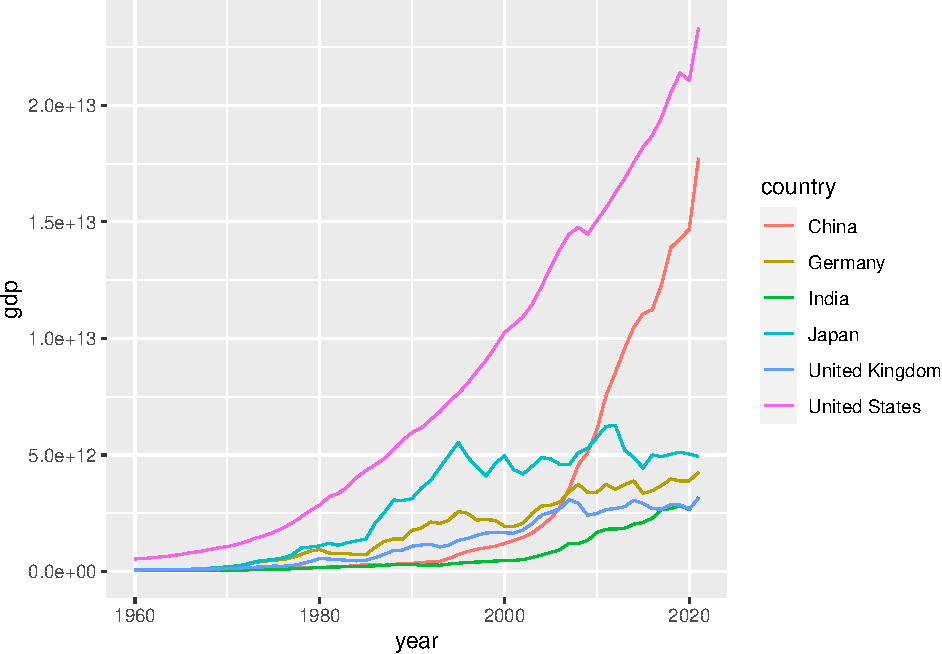
\includegraphics{31-worldbank_files/figure-latex/unnamed-chunk-39-1.pdf}

Warning として、missing values があると出ています。どこかは、分かりませんが、図を書くときですから、\texttt{y} に対応する、\texttt{gdp} の値がないものと思われます。

\hypertarget{ux30b0ux30e9ux30d5-2}{%
\section{グラフ 2}\label{ux30b0ux30e9ux30d5-2}}

\texttt{drop\_na(gdp)} で、\texttt{gdp} の値が、NA であるものを削除します。また、\texttt{labs} で、図にタイトルをつけます。

\begin{Shaded}
\begin{Highlighting}[]
\NormalTok{df\_gdp4 }\SpecialCharTok{\%\textgreater{}\%} \FunctionTok{drop\_na}\NormalTok{(gdp) }\SpecialCharTok{\%\textgreater{}\%} 
  \FunctionTok{ggplot}\NormalTok{(}\FunctionTok{aes}\NormalTok{(year, gdp, }\AttributeTok{col=}\NormalTok{country)) }\SpecialCharTok{+} \FunctionTok{geom\_line}\NormalTok{() }\SpecialCharTok{+}
  \FunctionTok{labs}\NormalTok{(}\AttributeTok{title =} \StringTok{"WDI {-} NY.GDP.MKTP.CD: gdp"}\NormalTok{)}
\end{Highlighting}
\end{Shaded}

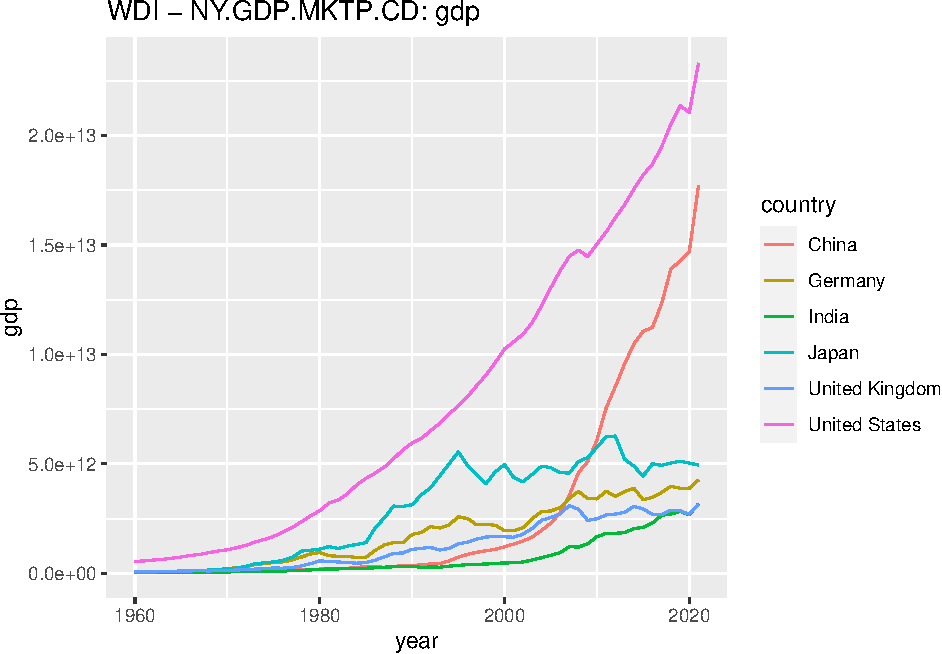
\includegraphics{31-worldbank_files/figure-latex/unnamed-chunk-40-1.pdf}

\hypertarget{ux30c6ux30f3ux30d7ux30ecux30fcux30c8-templates}{%
\section{テンプレート Templates}\label{ux30c6ux30f3ux30d7ux30ecux30fcux30c8-templates}}

下に、テンプレートをつけます。コピーして、指標コードや、略称、国などを、それぞれ置き換えて、試して見てください。少し、複雑な変形をしていますが、少しずつ説明します。

\hypertarget{ux4e00ux3064ux306eux56fdux306bux3064ux3044ux3066ux306eux4e00ux3064ux306eux6307ux6a19wdiux3068ux305dux306eux7565ux79f0ux304bux3089ux6298ux7ddaux30b0ux30e9ux30d5ux3092ux4f5cux6210}{%
\subsection{一つの国についての、一つの指標(WDI)と、その略称から、折線グラフを作成}\label{ux4e00ux3064ux306eux56fdux306bux3064ux3044ux3066ux306eux4e00ux3064ux306eux6307ux6a19wdiux3068ux305dux306eux7565ux79f0ux304bux3089ux6298ux7ddaux30b0ux30e9ux30d5ux3092ux4f5cux6210}}

Line Plot with one indicator with abbreviation and one country

\begin{Shaded}
\begin{Highlighting}[]
\NormalTok{chosen\_indicator }\OtherTok{\textless{}{-}} \StringTok{"SL.UEM.TOTL.NE.ZS"}
\NormalTok{short\_name }\OtherTok{\textless{}{-}} \StringTok{"unemployment"}
\NormalTok{chosen\_country }\OtherTok{\textless{}{-}} \StringTok{"United States"}
\FunctionTok{WDI}\NormalTok{(}\AttributeTok{country =} \StringTok{"all"}\NormalTok{, }\AttributeTok{indicator =} \FunctionTok{c}\NormalTok{(}\AttributeTok{short\_name =}\NormalTok{ chosen\_indicator), }\AttributeTok{extra=}\ConstantTok{TRUE}\NormalTok{, }\AttributeTok{cache=}\NormalTok{wdi\_cache) }\SpecialCharTok{\%\textgreater{}\%}
  \FunctionTok{filter}\NormalTok{(country }\SpecialCharTok{==}\NormalTok{ chosen\_country) }\SpecialCharTok{\%\textgreater{}\%} 
  \FunctionTok{ggplot}\NormalTok{(}\FunctionTok{aes}\NormalTok{(year, short\_name)) }\SpecialCharTok{+} \FunctionTok{geom\_line}\NormalTok{() }\SpecialCharTok{+}
  \FunctionTok{labs}\NormalTok{(}\AttributeTok{title =} \FunctionTok{paste}\NormalTok{(}\StringTok{"WDI "}\NormalTok{, chosen\_indicator, }\StringTok{": "}\NormalTok{, short\_name, }\StringTok{" {-} "}\NormalTok{, chosen\_country),}
       \AttributeTok{y =}\NormalTok{ short\_name)}
\end{Highlighting}
\end{Shaded}

\hypertarget{ux4e00ux3064ux306eux56fdux306bux3064ux3044ux3066ux306eux4e00ux3064ux306eux6307ux6a19wdiux304bux3089ux6298ux7ddaux30b0ux30e9ux30d5ux3092ux4f5cux6210}{%
\subsection{一つの国についての、一つの指標(WDI)から、折線グラフを作成}\label{ux4e00ux3064ux306eux56fdux306bux3064ux3044ux3066ux306eux4e00ux3064ux306eux6307ux6a19wdiux304bux3089ux6298ux7ddaux30b0ux30e9ux30d5ux3092ux4f5cux6210}}

Line Plot with one indicator and one country

\begin{Shaded}
\begin{Highlighting}[]
\NormalTok{chosen\_indicator }\OtherTok{\textless{}{-}} \StringTok{"SL.UEM.TOTL.NE.ZS"}
\NormalTok{chosen\_country }\OtherTok{\textless{}{-}} \StringTok{"United States"}
\FunctionTok{WDI}\NormalTok{(}\AttributeTok{country =} \StringTok{"all"}\NormalTok{, }\AttributeTok{indicator =} \FunctionTok{c}\NormalTok{(}\AttributeTok{chosen\_indicator =}\NormalTok{ chosen\_indicator), }
    \AttributeTok{extra=}\ConstantTok{TRUE}\NormalTok{, }\AttributeTok{cache=}\NormalTok{wdi\_cache) }\SpecialCharTok{\%\textgreater{}\%}
  \FunctionTok{filter}\NormalTok{(country }\SpecialCharTok{==}\NormalTok{ chosen\_country) }\SpecialCharTok{\%\textgreater{}\%} 
  \FunctionTok{ggplot}\NormalTok{(}\FunctionTok{aes}\NormalTok{(year, chosen\_indicator)) }\SpecialCharTok{+} \FunctionTok{geom\_line}\NormalTok{() }\SpecialCharTok{+}
  \FunctionTok{labs}\NormalTok{(}\AttributeTok{title =} \FunctionTok{paste}\NormalTok{(}\StringTok{"WDI "}\NormalTok{, chosen\_indicator, }\StringTok{" {-} "}\NormalTok{, chosen\_country), }
       \AttributeTok{y =}\NormalTok{ chosen\_indicator)}
\end{Highlighting}
\end{Shaded}

\hypertarget{ux3044ux304fux3064ux304bux306eux56fdux306bux3064ux3044ux3066ux306eux4e00ux3064ux306eux6307ux6a19wdiux3068ux305dux306eux7565ux79f0ux304bux3089ux6298ux7ddaux30b0ux30e9ux30d5ux3092ux4f5cux6210}{%
\subsection{いくつかの国についての、一つの指標(WDI)と、その略称から、折線グラフを作成}\label{ux3044ux304fux3064ux304bux306eux56fdux306bux3064ux3044ux3066ux306eux4e00ux3064ux306eux6307ux6a19wdiux3068ux305dux306eux7565ux79f0ux304bux3089ux6298ux7ddaux30b0ux30e9ux30d5ux3092ux4f5cux6210}}

Line Plot with one indicator with abbreviation and several countries

\begin{Shaded}
\begin{Highlighting}[]
\NormalTok{chosen\_indicator }\OtherTok{\textless{}{-}} \StringTok{"SL.UEM.TOTL.NE.ZS"}
\NormalTok{short\_name }\OtherTok{\textless{}{-}} \StringTok{"unemployment"}
\NormalTok{chosen\_countries }\OtherTok{\textless{}{-}} \FunctionTok{c}\NormalTok{(}\StringTok{"United States"}\NormalTok{,}\StringTok{"United Kingdom"}\NormalTok{, }\StringTok{"Japan"}\NormalTok{)}
\FunctionTok{WDI}\NormalTok{(}\AttributeTok{country =} \StringTok{"all"}\NormalTok{, }\AttributeTok{indicator =} \FunctionTok{c}\NormalTok{(}\AttributeTok{short\_name =}\NormalTok{ chosen\_indicator), }\AttributeTok{extra=}\ConstantTok{TRUE}\NormalTok{, }\AttributeTok{cache=}\NormalTok{wdi\_cache) }\SpecialCharTok{\%\textgreater{}\%} \FunctionTok{drop\_na}\NormalTok{(short\_name) }\SpecialCharTok{\%\textgreater{}\%} 
  \FunctionTok{filter}\NormalTok{(country }\SpecialCharTok{\%in\%}\NormalTok{ chosen\_countries) }\SpecialCharTok{\%\textgreater{}\%} 
  \FunctionTok{ggplot}\NormalTok{(}\FunctionTok{aes}\NormalTok{(year, short\_name, }\AttributeTok{col =}\NormalTok{ country)) }\SpecialCharTok{+} \FunctionTok{geom\_line}\NormalTok{() }\SpecialCharTok{+}
  \FunctionTok{labs}\NormalTok{(}\AttributeTok{title =} \FunctionTok{paste}\NormalTok{(}\StringTok{"WDI "}\NormalTok{, chosen\_indicator, }\StringTok{": "}\NormalTok{, short\_name), }\AttributeTok{y =}\NormalTok{ short\_name)}
\end{Highlighting}
\end{Shaded}

\hypertarget{ux4e00ux3064ux306eux56fdux306bux3064ux3044ux3066ux306eux4e8cux3064ux306eux6307ux6a19wdiux3068ux305dux306eux7565ux79f0ux304bux3089ux6298ux7ddaux30b0ux30e9ux30d5ux3092ux4f5cux6210}{%
\subsection{一つの国についての、二つの指標(WDI)と、その略称から、折線グラフを作成}\label{ux4e00ux3064ux306eux56fdux306bux3064ux3044ux3066ux306eux4e8cux3064ux306eux6307ux6a19wdiux3068ux305dux306eux7565ux79f0ux304bux3089ux6298ux7ddaux30b0ux30e9ux30d5ux3092ux4f5cux6210}}

Line Plot with two indicators with abbreviation and one country

\begin{Shaded}
\begin{Highlighting}[]
\NormalTok{chosen\_indicator\_1 }\OtherTok{\textless{}{-}} \StringTok{"NY.GDP.DEFL.KD.ZG"}
\NormalTok{short\_name\_1 }\OtherTok{\textless{}{-}} \StringTok{"gdp\_deflator"}
\NormalTok{chosen\_indicator\_2 }\OtherTok{\textless{}{-}} \StringTok{"CPTOTSAXNZGY"}
\NormalTok{short\_name\_2 }\OtherTok{\textless{}{-}} \StringTok{"cpi\_price"}
\NormalTok{chosen\_country }\OtherTok{\textless{}{-}} \StringTok{"United States"}
\FunctionTok{WDI}\NormalTok{(}\AttributeTok{country =} \StringTok{"all"}\NormalTok{, }\AttributeTok{indicator =} \FunctionTok{c}\NormalTok{(}\AttributeTok{short\_name\_1 =}\NormalTok{ chosen\_indicator\_1, }\AttributeTok{short\_name\_2 =}\NormalTok{ chosen\_indicator\_2), }\AttributeTok{extra=}\ConstantTok{TRUE}\NormalTok{, }\AttributeTok{cache=}\NormalTok{wdi\_cache) }\SpecialCharTok{\%\textgreater{}\%} 
  \FunctionTok{filter}\NormalTok{(country }\SpecialCharTok{==}\NormalTok{ chosen\_country) }\SpecialCharTok{\%\textgreater{}\%} 
  \FunctionTok{pivot\_longer}\NormalTok{(}\FunctionTok{c}\NormalTok{(short\_name\_1, short\_name\_2), }\AttributeTok{names\_to =} \StringTok{"class"}\NormalTok{, }\AttributeTok{values\_to =} \StringTok{"value"}\NormalTok{) }\SpecialCharTok{\%\textgreater{}\%} \FunctionTok{drop\_na}\NormalTok{(value) }\SpecialCharTok{\%\textgreater{}\%}
  \FunctionTok{ggplot}\NormalTok{(}\FunctionTok{aes}\NormalTok{(year, value, }\AttributeTok{col =}\NormalTok{ class)) }\SpecialCharTok{+} \FunctionTok{geom\_line}\NormalTok{() }\SpecialCharTok{+}
  \FunctionTok{labs}\NormalTok{(}\AttributeTok{title =} \FunctionTok{paste}\NormalTok{(}\StringTok{"WDI "}\NormalTok{, chosen\_indicator\_1, }\StringTok{": "}\NormalTok{, short\_name\_1, }\StringTok{"}\SpecialCharTok{\textbackslash{}n}\StringTok{"}\NormalTok{, chosen\_indicator\_2, }\StringTok{": "}\NormalTok{, short\_name\_2, }\StringTok{" {-} "}\NormalTok{, chosen\_country)) }\SpecialCharTok{+}
  \FunctionTok{scale\_color\_manual}\NormalTok{(}\AttributeTok{labels =} \FunctionTok{c}\NormalTok{(short\_name\_1, short\_name\_2), }\AttributeTok{values =}\NormalTok{ scales}\SpecialCharTok{::}\FunctionTok{hue\_pal}\NormalTok{()(}\DecValTok{2}\NormalTok{))}
\end{Highlighting}
\end{Shaded}

\begin{Shaded}
\begin{Highlighting}[]
\NormalTok{chosen\_indicator\_1 }\OtherTok{\textless{}{-}} \StringTok{"SL.TLF.CACT.MA.NE.ZS"}
\NormalTok{short\_name\_1 }\OtherTok{\textless{}{-}} \StringTok{"male"}
\NormalTok{chosen\_indicator\_2 }\OtherTok{\textless{}{-}} \StringTok{"SL.TLF.CACT.FE.NE.ZS"}
\NormalTok{short\_name\_2 }\OtherTok{\textless{}{-}} \StringTok{"female"}
\NormalTok{chosen\_country }\OtherTok{\textless{}{-}} \StringTok{"United States"}
\FunctionTok{WDI}\NormalTok{(}\AttributeTok{country =} \StringTok{"all"}\NormalTok{, }\AttributeTok{indicator =} \FunctionTok{c}\NormalTok{(}\AttributeTok{short\_name\_1 =}\NormalTok{ chosen\_indicator\_1, }\AttributeTok{short\_name\_2 =}\NormalTok{ chosen\_indicator\_2), }\AttributeTok{extra=}\ConstantTok{TRUE}\NormalTok{, }\AttributeTok{cache=}\NormalTok{wdi\_cache) }\SpecialCharTok{\%\textgreater{}\%} 
  \FunctionTok{filter}\NormalTok{(country }\SpecialCharTok{==}\NormalTok{ chosen\_country) }\SpecialCharTok{\%\textgreater{}\%} 
  \FunctionTok{pivot\_longer}\NormalTok{(}\FunctionTok{c}\NormalTok{(short\_name\_1, short\_name\_2), }\AttributeTok{names\_to =} \StringTok{"class"}\NormalTok{, }\AttributeTok{values\_to =} \StringTok{"value"}\NormalTok{) }\SpecialCharTok{\%\textgreater{}\%} \FunctionTok{drop\_na}\NormalTok{(value) }\SpecialCharTok{\%\textgreater{}\%}
  \FunctionTok{ggplot}\NormalTok{(}\FunctionTok{aes}\NormalTok{(year, value, }\AttributeTok{col =}\NormalTok{ class)) }\SpecialCharTok{+} \FunctionTok{geom\_line}\NormalTok{() }\SpecialCharTok{+}
  \FunctionTok{labs}\NormalTok{(}\AttributeTok{title =} \FunctionTok{paste}\NormalTok{(}\StringTok{"WDI "}\NormalTok{, chosen\_indicator\_1, }\StringTok{": "}\NormalTok{, short\_name\_1, }\StringTok{"}\SpecialCharTok{\textbackslash{}n}\StringTok{"}\NormalTok{, chosen\_indicator\_2, }\StringTok{": "}\NormalTok{, short\_name\_2, }\StringTok{" {-} "}\NormalTok{, chosen\_country)) }\SpecialCharTok{+}
  \FunctionTok{scale\_color\_manual}\NormalTok{(}\AttributeTok{labels =} \FunctionTok{c}\NormalTok{(short\_name\_1, short\_name\_2), }\AttributeTok{values =}\NormalTok{ scales}\SpecialCharTok{::}\FunctionTok{hue\_pal}\NormalTok{()(}\DecValTok{2}\NormalTok{))}
\end{Highlighting}
\end{Shaded}

\hypertarget{ux3044ux304fux3064ux304bux306eux56fdux306bux3064ux3044ux3066ux306eux4e8cux3064ux306eux6307ux6a19wdiux3068ux305dux306eux7565ux79f0ux304bux3089ux6298ux7ddaux30b0ux30e9ux30d5ux3092ux4f5cux6210}{%
\subsection{いくつかの国についての、二つの指標(WDI)と、その略称から、折線グラフを作成}\label{ux3044ux304fux3064ux304bux306eux56fdux306bux3064ux3044ux3066ux306eux4e8cux3064ux306eux6307ux6a19wdiux3068ux305dux306eux7565ux79f0ux304bux3089ux6298ux7ddaux30b0ux30e9ux30d5ux3092ux4f5cux6210}}

Line Plot with two indicators with abbreviation and several countries

\begin{Shaded}
\begin{Highlighting}[]
\NormalTok{chosen\_indicator\_1 }\OtherTok{\textless{}{-}} \StringTok{"NY.GDP.DEFL.KD.ZG"}
\NormalTok{short\_name\_1 }\OtherTok{\textless{}{-}} \StringTok{"gdp\_deflator"}
\NormalTok{chosen\_indicator\_2 }\OtherTok{\textless{}{-}} \StringTok{"CPTOTSAXNZGY"}
\NormalTok{short\_name\_2 }\OtherTok{\textless{}{-}} \StringTok{"cpi\_price"}
\NormalTok{chosen\_countries }\OtherTok{\textless{}{-}} \FunctionTok{c}\NormalTok{(}\StringTok{"United States"}\NormalTok{, }\StringTok{"France"}\NormalTok{, }\StringTok{"Japan"}\NormalTok{)}
\FunctionTok{WDI}\NormalTok{(}\AttributeTok{country =} \StringTok{"all"}\NormalTok{, }\AttributeTok{indicator =} \FunctionTok{c}\NormalTok{(}\AttributeTok{short\_name\_1 =}\NormalTok{ chosen\_indicator\_1, }\AttributeTok{short\_name\_2 =}\NormalTok{ chosen\_indicator\_2), }\AttributeTok{extra=}\ConstantTok{TRUE}\NormalTok{, }\AttributeTok{cache=}\NormalTok{wdi\_cache) }\SpecialCharTok{\%\textgreater{}\%} 
  \FunctionTok{filter}\NormalTok{(country }\SpecialCharTok{\%in\%}\NormalTok{ chosen\_countries) }\SpecialCharTok{\%\textgreater{}\%} 
  \FunctionTok{pivot\_longer}\NormalTok{(}\FunctionTok{c}\NormalTok{(short\_name\_1, short\_name\_2), }\AttributeTok{names\_to =} \StringTok{"class"}\NormalTok{, }\AttributeTok{values\_to =} \StringTok{"value"}\NormalTok{) }\SpecialCharTok{\%\textgreater{}\%} \FunctionTok{drop\_na}\NormalTok{(value) }\SpecialCharTok{\%\textgreater{}\%}
  \FunctionTok{ggplot}\NormalTok{(}\FunctionTok{aes}\NormalTok{(year, value, }\AttributeTok{linetype =}\NormalTok{ class, }\AttributeTok{col =}\NormalTok{ country)) }\SpecialCharTok{+} \FunctionTok{geom\_line}\NormalTok{() }\SpecialCharTok{+}
  \FunctionTok{labs}\NormalTok{(}\AttributeTok{title =} \FunctionTok{paste}\NormalTok{(}\StringTok{"WDI "}\NormalTok{, chosen\_indicator\_1, }\StringTok{": "}\NormalTok{, short\_name\_1, }\StringTok{"}\SpecialCharTok{\textbackslash{}n}\StringTok{"}\NormalTok{, chosen\_indicator\_2, }\StringTok{": "}\NormalTok{, short\_name\_2)) }\SpecialCharTok{+}
  \FunctionTok{scale\_linetype\_manual}\NormalTok{(}\AttributeTok{labels =} \FunctionTok{c}\NormalTok{(short\_name\_1, short\_name\_2), }\AttributeTok{values =} \FunctionTok{c}\NormalTok{(}\StringTok{"solid"}\NormalTok{, }\StringTok{"dashed"}\NormalTok{))}
\end{Highlighting}
\end{Shaded}

\begin{Shaded}
\begin{Highlighting}[]
\NormalTok{chosen\_indicator\_1 }\OtherTok{\textless{}{-}} \StringTok{"SL.TLF.CACT.MA.NE.ZS"}
\NormalTok{short\_name\_1 }\OtherTok{\textless{}{-}} \StringTok{"male"}
\NormalTok{chosen\_indicator\_2 }\OtherTok{\textless{}{-}} \StringTok{"SL.TLF.CACT.FE.NE.ZS"}
\NormalTok{short\_name\_2 }\OtherTok{\textless{}{-}} \StringTok{"female"}
\NormalTok{chosen\_countries }\OtherTok{\textless{}{-}} \FunctionTok{c}\NormalTok{(}\StringTok{"United States"}\NormalTok{, }\StringTok{"France"}\NormalTok{, }\StringTok{"Japan"}\NormalTok{)}
\FunctionTok{WDI}\NormalTok{(}\AttributeTok{country =} \StringTok{"all"}\NormalTok{, }\AttributeTok{indicator =} \FunctionTok{c}\NormalTok{(}\AttributeTok{short\_name\_1 =}\NormalTok{ chosen\_indicator\_1, }\AttributeTok{short\_name\_2 =}\NormalTok{ chosen\_indicator\_2), }\AttributeTok{extra=}\ConstantTok{TRUE}\NormalTok{, }\AttributeTok{cache=}\NormalTok{wdi\_cache) }\SpecialCharTok{\%\textgreater{}\%} 
  \FunctionTok{filter}\NormalTok{(country }\SpecialCharTok{\%in\%}\NormalTok{ chosen\_countries) }\SpecialCharTok{\%\textgreater{}\%} 
  \FunctionTok{pivot\_longer}\NormalTok{(}\FunctionTok{c}\NormalTok{(short\_name\_1, short\_name\_2), }\AttributeTok{names\_to =} \StringTok{"class"}\NormalTok{, }\AttributeTok{values\_to =} \StringTok{"value"}\NormalTok{) }\SpecialCharTok{\%\textgreater{}\%} \FunctionTok{drop\_na}\NormalTok{(value) }\SpecialCharTok{\%\textgreater{}\%}
  \FunctionTok{ggplot}\NormalTok{(}\FunctionTok{aes}\NormalTok{(year, value, }\AttributeTok{linetype =}\NormalTok{ class, }\AttributeTok{col =}\NormalTok{ country)) }\SpecialCharTok{+} \FunctionTok{geom\_line}\NormalTok{() }\SpecialCharTok{+}
  \FunctionTok{labs}\NormalTok{(}\AttributeTok{title =} \FunctionTok{paste}\NormalTok{(}\StringTok{"WDI "}\NormalTok{, chosen\_indicator\_1, }\StringTok{": "}\NormalTok{, short\_name\_1, }\StringTok{"}\SpecialCharTok{\textbackslash{}n}\StringTok{"}\NormalTok{, chosen\_indicator\_2, }\StringTok{": "}\NormalTok{, short\_name\_2)) }\SpecialCharTok{+}
  \FunctionTok{scale\_linetype\_manual}\NormalTok{(}\AttributeTok{labels =} \FunctionTok{c}\NormalTok{(short\_name\_1, short\_name\_2), }\AttributeTok{values =} \FunctionTok{c}\NormalTok{(}\StringTok{"solid"}\NormalTok{, }\StringTok{"dashed"}\NormalTok{))}
\end{Highlighting}
\end{Shaded}

\hypertarget{ux8ab2ux984c-assignment}{%
\chapter{課題 Assignment}\label{ux8ab2ux984c-assignment}}

上のテンプレートをコピーして、下に貼り付け、指標 \texttt{indicator} と、略称 \texttt{short\_name} と、いくつかの国名 \texttt{chosen\_countries} を、入れ替えて、試してみてください。

\hypertarget{part-part-iv-eda}{%
\part*{(PART) PART IV EDA}\label{part-part-iv-eda}}
\addcontentsline{toc}{part}{(PART) PART IV EDA}

\hypertarget{intro2eda}{%
\part{探索的データ解析}\label{intro2eda}}

\hypertarget{ux63a2ux7d22ux7684ux30c7ux30fcux30bfux89e3ux6790-edaux3068ux306f}{%
\chapter{探索的データ解析 (EDA)とは}\label{ux63a2ux7d22ux7684ux30c7ux30fcux30bfux89e3ux6790-edaux3068ux306f}}

\begin{figure}
\centering
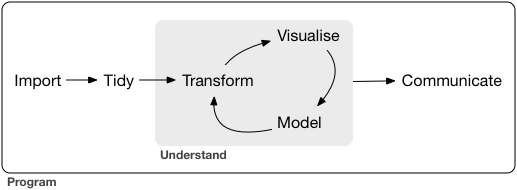
\includegraphics{./data/data-science.png}
\caption{image from r4ds}
\end{figure}

以下は、\href{https://posit.cloud/learn/primers/3.1}{Posit Primers: Visualise Data} から

探索的データ解析 (EDA) は、データを理解するための反復的なサイクルです。EDAでは、以下のことを行います。

\begin{enumerate}
\def\labelenumi{\arabic{enumi}.}
\item
  データに関する問いを作成する
\item
  データの可視化、変形・整形、モデリングによって、問いの答えを探索する。
\item
  学んだことを使って、問いをより洗練されたものとする。
\end{enumerate}

EDAは、あらゆるデータ分析において重要な役割を担います。EDA によって、課題解決のいとぐちを発見することもありますし、他の課題との関係性を発見する場合もあります。EDAを使用してデータの問題や品質を確認したり、データが信頼できるものであるかを見極める問いを作成できる場合もあります。

\hypertarget{ux63a2ux7d22ux7684ux30c7ux30fcux30bfux89e3ux6790-eda-ux306eux4e00ux4f8b}{%
\chapter{探索的データ解析 (EDA) の一例}\label{ux63a2ux7d22ux7684ux30c7ux30fcux30bfux89e3ux6790-eda-ux306eux4e00ux4f8b}}

WDI の一つの指標を使って、流れを見てみましょう。

\hypertarget{ux30c7ux30fcux30bfux306eux53d6ux5f97ux3068ux8aadux307fux8fbcux307f---data-import}{%
\section{データの取得と読み込み - Data Import}\label{ux30c7ux30fcux30bfux306eux53d6ux5f97ux3068ux8aadux307fux8fbcux307f---data-import}}

NY.GDP.PCAP.CD: GDP per capita (current US\$)

\begin{Shaded}
\begin{Highlighting}[]
\NormalTok{df\_wdi\_gdppcap }\OtherTok{\textless{}{-}} \FunctionTok{WDI}\NormalTok{(}\AttributeTok{country =} \StringTok{"all"}\NormalTok{, }\AttributeTok{indicator =} \FunctionTok{c}\NormalTok{(}\AttributeTok{gdp\_pcap =} \StringTok{"NY.GDP.PCAP.CD"}\NormalTok{))}
\FunctionTok{write\_csv}\NormalTok{(df\_wdi\_gdppcap, }\StringTok{"./data/df\_wdi\_gdppcap.csv"}\NormalTok{)}
\end{Highlighting}
\end{Shaded}

\begin{Shaded}
\begin{Highlighting}[]
\NormalTok{df\_wdi\_gdppcap}
\CommentTok{\#\textgreater{} \# A tibble: 16,492 x 5}
\CommentTok{\#\textgreater{}    country                     iso2c iso3c  year gdp\_pcap}
\CommentTok{\#\textgreater{}    \textless{}chr\textgreater{}                       \textless{}chr\textgreater{} \textless{}chr\textgreater{} \textless{}dbl\textgreater{}    \textless{}dbl\textgreater{}}
\CommentTok{\#\textgreater{}  1 Africa Eastern and Southern ZH    AFE    2021    1550.}
\CommentTok{\#\textgreater{}  2 Africa Eastern and Southern ZH    AFE    2020    1364.}
\CommentTok{\#\textgreater{}  3 Africa Eastern and Southern ZH    AFE    2019    1512.}
\CommentTok{\#\textgreater{}  4 Africa Eastern and Southern ZH    AFE    2018    1565.}
\CommentTok{\#\textgreater{}  5 Africa Eastern and Southern ZH    AFE    2017    1629.}
\CommentTok{\#\textgreater{}  6 Africa Eastern and Southern ZH    AFE    2016    1444.}
\CommentTok{\#\textgreater{}  7 Africa Eastern and Southern ZH    AFE    2015    1539.}
\CommentTok{\#\textgreater{}  8 Africa Eastern and Southern ZH    AFE    2014    1719.}
\CommentTok{\#\textgreater{}  9 Africa Eastern and Southern ZH    AFE    2013    1730.}
\CommentTok{\#\textgreater{} 10 Africa Eastern and Southern ZH    AFE    2012    1759.}
\CommentTok{\#\textgreater{} \# ... with 16,482 more rows}
\end{Highlighting}
\end{Shaded}

\hypertarget{ux30c7ux30fcux30bfux5909ux5f62ux6574ux5f62---data-transformation}{%
\section{データ変形・整形 - Data Transformation}\label{ux30c7ux30fcux30bfux5909ux5f62ux6574ux5f62---data-transformation}}

\hypertarget{ux5217ux3092-select}{%
\subsection{\texorpdfstring{列を \texttt{select}}{列を select}}\label{ux5217ux3092-select}}

どの変数について分析するかを選ぶ。

\begin{Shaded}
\begin{Highlighting}[]
\NormalTok{df\_wdi\_gdppcap\_small }\OtherTok{\textless{}{-}}\NormalTok{ df\_wdi\_gdppcap }\SpecialCharTok{\%\textgreater{}\%} 
  \FunctionTok{select}\NormalTok{(country, year, gdp\_pcap)}
\NormalTok{df\_wdi\_gdppcap\_small}
\CommentTok{\#\textgreater{} \# A tibble: 16,492 x 3}
\CommentTok{\#\textgreater{}    country                      year gdp\_pcap}
\CommentTok{\#\textgreater{}    \textless{}chr\textgreater{}                       \textless{}dbl\textgreater{}    \textless{}dbl\textgreater{}}
\CommentTok{\#\textgreater{}  1 Africa Eastern and Southern  2021    1550.}
\CommentTok{\#\textgreater{}  2 Africa Eastern and Southern  2020    1364.}
\CommentTok{\#\textgreater{}  3 Africa Eastern and Southern  2019    1512.}
\CommentTok{\#\textgreater{}  4 Africa Eastern and Southern  2018    1565.}
\CommentTok{\#\textgreater{}  5 Africa Eastern and Southern  2017    1629.}
\CommentTok{\#\textgreater{}  6 Africa Eastern and Southern  2016    1444.}
\CommentTok{\#\textgreater{}  7 Africa Eastern and Southern  2015    1539.}
\CommentTok{\#\textgreater{}  8 Africa Eastern and Southern  2014    1719.}
\CommentTok{\#\textgreater{}  9 Africa Eastern and Southern  2013    1730.}
\CommentTok{\#\textgreater{} 10 Africa Eastern and Southern  2012    1759.}
\CommentTok{\#\textgreater{} \# ... with 16,482 more rows}
\end{Highlighting}
\end{Shaded}

\hypertarget{ux884cux3092-filter}{%
\subsection{\texorpdfstring{行を \texttt{filter}}{行を filter}}\label{ux884cux3092-filter}}

いくつかの国に、フォーカスして調べる。

\begin{Shaded}
\begin{Highlighting}[]
\NormalTok{df\_wdi\_gdppcap\_short }\OtherTok{\textless{}{-}}\NormalTok{ df\_wdi\_gdppcap }\SpecialCharTok{\%\textgreater{}\%} 
  \FunctionTok{filter}\NormalTok{(country }\SpecialCharTok{\%in\%} \FunctionTok{c}\NormalTok{(}\StringTok{"Japan"}\NormalTok{, }\StringTok{"Germany"}\NormalTok{, }\StringTok{"United States"}\NormalTok{))}
\NormalTok{df\_wdi\_gdppcap\_short}
\CommentTok{\#\textgreater{} \# A tibble: 186 x 5}
\CommentTok{\#\textgreater{}    country iso2c iso3c  year gdp\_pcap}
\CommentTok{\#\textgreater{}    \textless{}chr\textgreater{}   \textless{}chr\textgreater{} \textless{}chr\textgreater{} \textless{}dbl\textgreater{}    \textless{}dbl\textgreater{}}
\CommentTok{\#\textgreater{}  1 Germany DE    DEU    2021   51204.}
\CommentTok{\#\textgreater{}  2 Germany DE    DEU    2020   46773.}
\CommentTok{\#\textgreater{}  3 Germany DE    DEU    2019   46794.}
\CommentTok{\#\textgreater{}  4 Germany DE    DEU    2018   47939.}
\CommentTok{\#\textgreater{}  5 Germany DE    DEU    2017   44653.}
\CommentTok{\#\textgreater{}  6 Germany DE    DEU    2016   42136.}
\CommentTok{\#\textgreater{}  7 Germany DE    DEU    2015   41103.}
\CommentTok{\#\textgreater{}  8 Germany DE    DEU    2014   48024.}
\CommentTok{\#\textgreater{}  9 Germany DE    DEU    2013   46299.}
\CommentTok{\#\textgreater{} 10 Germany DE    DEU    2012   43856.}
\CommentTok{\#\textgreater{} \# ... with 176 more rows}
\end{Highlighting}
\end{Shaded}

列(変数)と、行(国)の選択を続けて、実行すると次のようになる。 一つ一つ変形したデータ(オブジェクト)に名前をつけて、保存する必要がないので、パイプ(\texttt{\%\textgreater{}\%})の活用は有用である。

\begin{Shaded}
\begin{Highlighting}[]
\NormalTok{df\_wdi\_gdppcap\_small\_short }\OtherTok{\textless{}{-}}\NormalTok{ df\_wdi\_gdppcap }\SpecialCharTok{\%\textgreater{}\%} \FunctionTok{select}\NormalTok{(country, year, gdp\_pcap) }\SpecialCharTok{\%\textgreater{}\%}
  \FunctionTok{filter}\NormalTok{(country }\SpecialCharTok{\%in\%} \FunctionTok{c}\NormalTok{(}\StringTok{"Japan"}\NormalTok{, }\StringTok{"Germany"}\NormalTok{, }\StringTok{"United States"}\NormalTok{))}
\NormalTok{df\_wdi\_gdppcap\_small\_short}
\CommentTok{\#\textgreater{} \# A tibble: 186 x 3}
\CommentTok{\#\textgreater{}    country  year gdp\_pcap}
\CommentTok{\#\textgreater{}    \textless{}chr\textgreater{}   \textless{}dbl\textgreater{}    \textless{}dbl\textgreater{}}
\CommentTok{\#\textgreater{}  1 Germany  2021   51204.}
\CommentTok{\#\textgreater{}  2 Germany  2020   46773.}
\CommentTok{\#\textgreater{}  3 Germany  2019   46794.}
\CommentTok{\#\textgreater{}  4 Germany  2018   47939.}
\CommentTok{\#\textgreater{}  5 Germany  2017   44653.}
\CommentTok{\#\textgreater{}  6 Germany  2016   42136.}
\CommentTok{\#\textgreater{}  7 Germany  2015   41103.}
\CommentTok{\#\textgreater{}  8 Germany  2014   48024.}
\CommentTok{\#\textgreater{}  9 Germany  2013   46299.}
\CommentTok{\#\textgreater{} 10 Germany  2012   43856.}
\CommentTok{\#\textgreater{} \# ... with 176 more rows}
\end{Highlighting}
\end{Shaded}

\hypertarget{ux53efux8996ux5316-data-visualization}{%
\section{可視化 Data Visualization}\label{ux53efux8996ux5316-data-visualization}}

次は、よく生じる、誤りの例で、ノコギリの歯(sawtoothed)のようなギザギザ・グラフと呼ばれます。なぜこのようなことが起きているかわかりますか。

\begin{Shaded}
\begin{Highlighting}[]
\NormalTok{df\_wdi\_gdppcap\_small\_short }\SpecialCharTok{\%\textgreater{}\%}
  \FunctionTok{ggplot}\NormalTok{(}\FunctionTok{aes}\NormalTok{(}\AttributeTok{x =}\NormalTok{ year, }\AttributeTok{y =}\NormalTok{ gdp\_pcap)) }\SpecialCharTok{+} \FunctionTok{geom\_line}\NormalTok{()}
\CommentTok{\#\textgreater{} Warning: Removed 1 row containing missing values}
\CommentTok{\#\textgreater{} (\textasciigrave{}geom\_line()\textasciigrave{}).}
\end{Highlighting}
\end{Shaded}

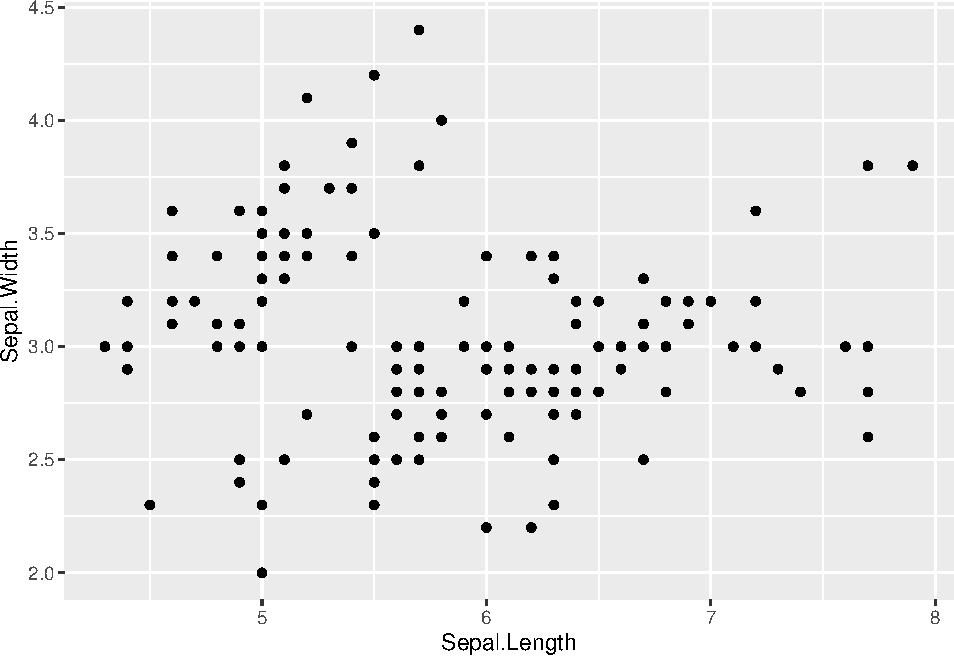
\includegraphics{41-eda_files/figure-latex/unnamed-chunk-9-1.pdf}

同じ年に、多くのデータがあるので、折れ線グラフを適切に書くことができませんでした。

\begin{Shaded}
\begin{Highlighting}[]
\NormalTok{df\_wdi\_gdppcap\_small\_short }\SpecialCharTok{\%\textgreater{}\%} \FunctionTok{filter}\NormalTok{(country }\SpecialCharTok{\%in\%} \FunctionTok{c}\NormalTok{(}\StringTok{"Japan"}\NormalTok{)) }\SpecialCharTok{\%\textgreater{}\%}
  \FunctionTok{ggplot}\NormalTok{(}\FunctionTok{aes}\NormalTok{(}\AttributeTok{x =}\NormalTok{ year, }\AttributeTok{y =}\NormalTok{ gdp\_pcap)) }\SpecialCharTok{+} \FunctionTok{geom\_line}\NormalTok{()}
\end{Highlighting}
\end{Shaded}

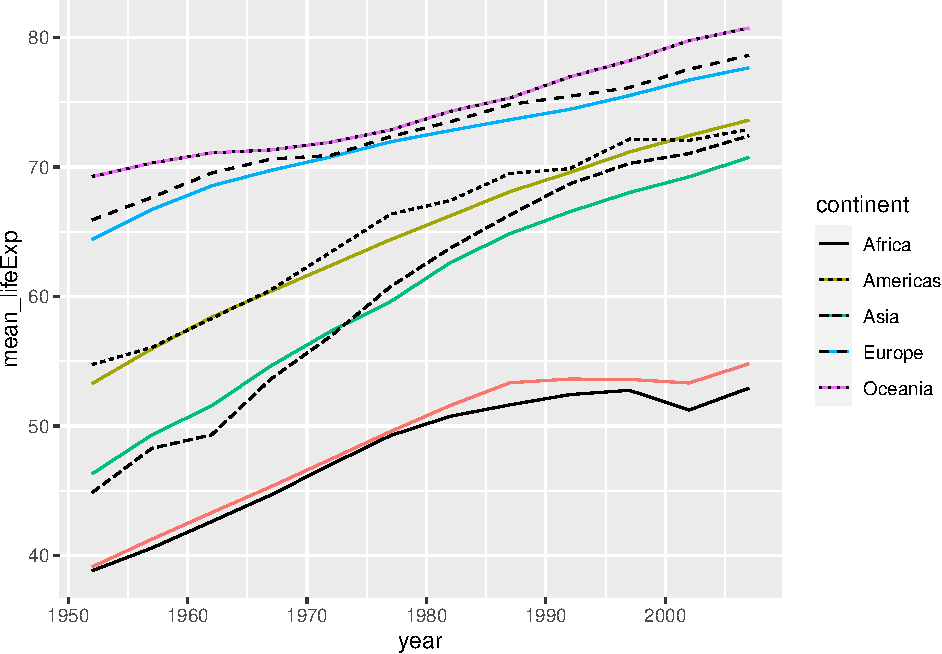
\includegraphics{41-eda_files/figure-latex/unnamed-chunk-10-1.pdf}

一般的には、散布図をまず、書いてみるのも一つです。

\begin{Shaded}
\begin{Highlighting}[]
\NormalTok{df\_wdi\_gdppcap\_small\_short }\SpecialCharTok{\%\textgreater{}\%}
  \FunctionTok{ggplot}\NormalTok{(}\FunctionTok{aes}\NormalTok{(}\AttributeTok{x =}\NormalTok{ year, }\AttributeTok{y =}\NormalTok{ gdp\_pcap)) }\SpecialCharTok{+} \FunctionTok{geom\_point}\NormalTok{()}
\CommentTok{\#\textgreater{} Warning: Removed 10 rows containing missing values}
\CommentTok{\#\textgreater{} (\textasciigrave{}geom\_point()\textasciigrave{}).}
\end{Highlighting}
\end{Shaded}

\includegraphics{41-eda_files/figure-latex/unnamed-chunk-11-1.pdf}

国別に、異なる色を使うことで、折れ線グラフを書くことも可能です。

\begin{Shaded}
\begin{Highlighting}[]
\NormalTok{df\_wdi\_gdppcap\_small\_short }\SpecialCharTok{\%\textgreater{}\%} \FunctionTok{drop\_na}\NormalTok{(gdp\_pcap) }\SpecialCharTok{\%\textgreater{}\%}
  \FunctionTok{ggplot}\NormalTok{(}\FunctionTok{aes}\NormalTok{(}\AttributeTok{x =}\NormalTok{ year, }\AttributeTok{y =}\NormalTok{ gdp\_pcap, }\AttributeTok{col =}\NormalTok{ country)) }\SpecialCharTok{+} \FunctionTok{geom\_line}\NormalTok{()}
\end{Highlighting}
\end{Shaded}

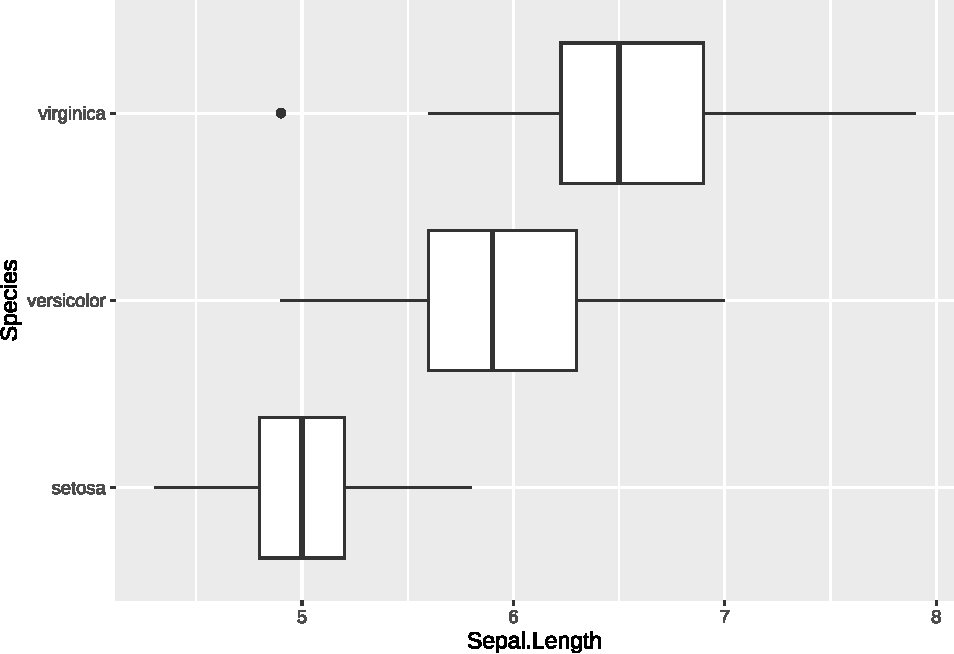
\includegraphics{41-eda_files/figure-latex/unnamed-chunk-12-1.pdf}

折線グラフと、散布図を同時に描くこともかのうです。

\begin{Shaded}
\begin{Highlighting}[]
\NormalTok{df\_wdi\_gdppcap\_small\_short }\SpecialCharTok{\%\textgreater{}\%} \FunctionTok{drop\_na}\NormalTok{(gdp\_pcap) }\SpecialCharTok{\%\textgreater{}\%}
  \FunctionTok{ggplot}\NormalTok{(}\FunctionTok{aes}\NormalTok{(}\AttributeTok{x =}\NormalTok{ year, }\AttributeTok{y =}\NormalTok{ gdp\_pcap, }\AttributeTok{col =}\NormalTok{ country)) }\SpecialCharTok{+} \FunctionTok{geom\_line}\NormalTok{() }\SpecialCharTok{+}
  \FunctionTok{geom\_point}\NormalTok{()}
\end{Highlighting}
\end{Shaded}

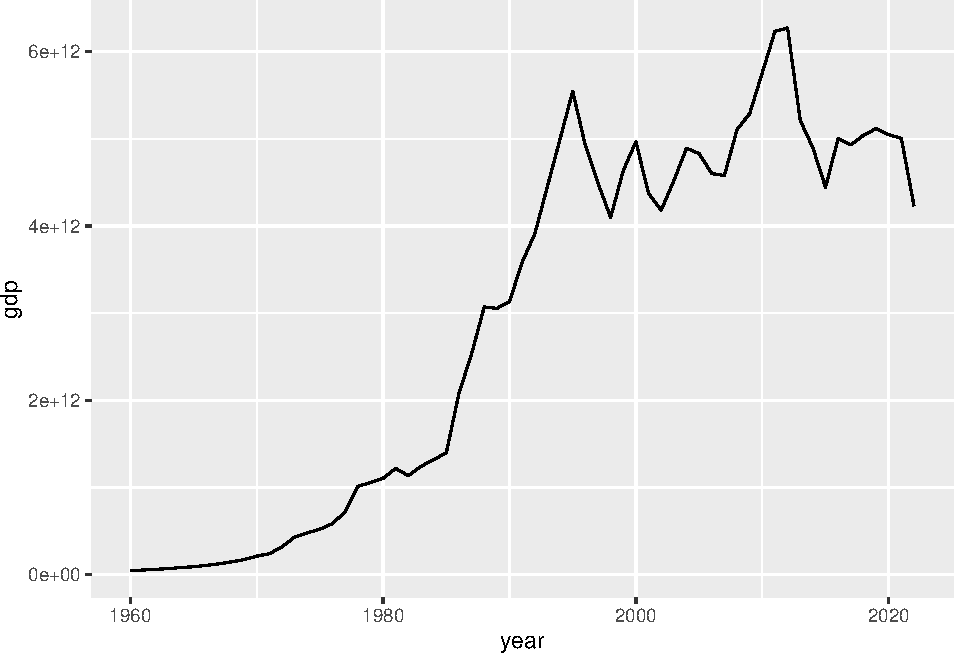
\includegraphics{41-eda_files/figure-latex/unnamed-chunk-13-1.pdf}

点を、曲線で近似する方法はいくつも知られているが、ある幅で、近似していく、LOESS が初期値となっている。\texttt{method=\textquotesingle{}loess\textquotesingle{}} を省略しても、同じ近似がなされる。\texttt{span} という値を調節することで、ことなる幅での近似曲線を書くことも可能である。初期値は、0.75。

\begin{Shaded}
\begin{Highlighting}[]
\NormalTok{df\_wdi\_gdppcap\_small\_short }\SpecialCharTok{\%\textgreater{}\%} \FunctionTok{drop\_na}\NormalTok{(gdp\_pcap) }\SpecialCharTok{\%\textgreater{}\%}
  \FunctionTok{ggplot}\NormalTok{(}\FunctionTok{aes}\NormalTok{(}\AttributeTok{x =}\NormalTok{ year, }\AttributeTok{y =}\NormalTok{ gdp\_pcap)) }\SpecialCharTok{+} 
  \FunctionTok{geom\_point}\NormalTok{(}\FunctionTok{aes}\NormalTok{(}\AttributeTok{color =}\NormalTok{ country)) }\SpecialCharTok{+} 
  \FunctionTok{geom\_smooth}\NormalTok{(}\AttributeTok{method =} \StringTok{\textquotesingle{}loess\textquotesingle{}}\NormalTok{, }\AttributeTok{formula =} \StringTok{\textquotesingle{}y \textasciitilde{} x\textquotesingle{}}\NormalTok{)}
\end{Highlighting}
\end{Shaded}

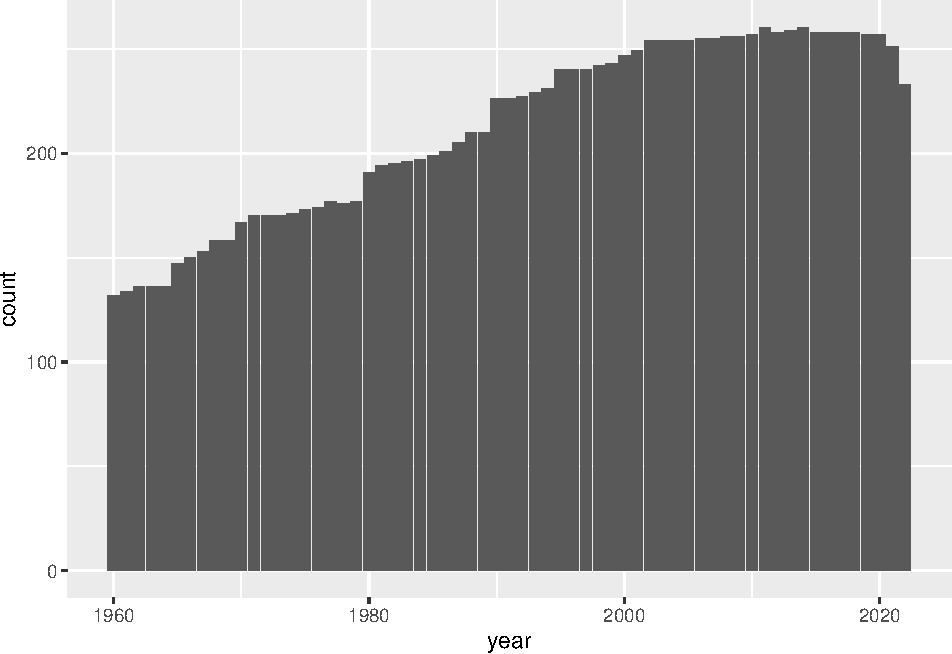
\includegraphics{41-eda_files/figure-latex/unnamed-chunk-14-1.pdf}

\hypertarget{ux30c7ux30fcux30bfux30e2ux30c7ux30eaux30f3ux30b0-data-modeling}{%
\section{データモデリング Data Modeling}\label{ux30c7ux30fcux30bfux30e2ux30c7ux30eaux30f3ux30b0-data-modeling}}

上の例では、曲線ではなく、直線で近似することも考えられる。

\begin{Shaded}
\begin{Highlighting}[]
\NormalTok{df\_wdi\_gdppcap\_small\_short }\SpecialCharTok{\%\textgreater{}\%} \FunctionTok{drop\_na}\NormalTok{(gdp\_pcap) }\SpecialCharTok{\%\textgreater{}\%}
  \FunctionTok{ggplot}\NormalTok{(}\FunctionTok{aes}\NormalTok{(}\AttributeTok{x =}\NormalTok{ year, }\AttributeTok{y =}\NormalTok{ gdp\_pcap)) }\SpecialCharTok{+} 
  \FunctionTok{geom\_point}\NormalTok{(}\FunctionTok{aes}\NormalTok{(}\AttributeTok{color =}\NormalTok{ country)) }\SpecialCharTok{+} 
  \FunctionTok{geom\_smooth}\NormalTok{(}\AttributeTok{method =} \StringTok{\textquotesingle{}lm\textquotesingle{}}\NormalTok{, }\AttributeTok{formula =} \StringTok{\textquotesingle{}y \textasciitilde{} x\textquotesingle{}}\NormalTok{)}
\end{Highlighting}
\end{Shaded}

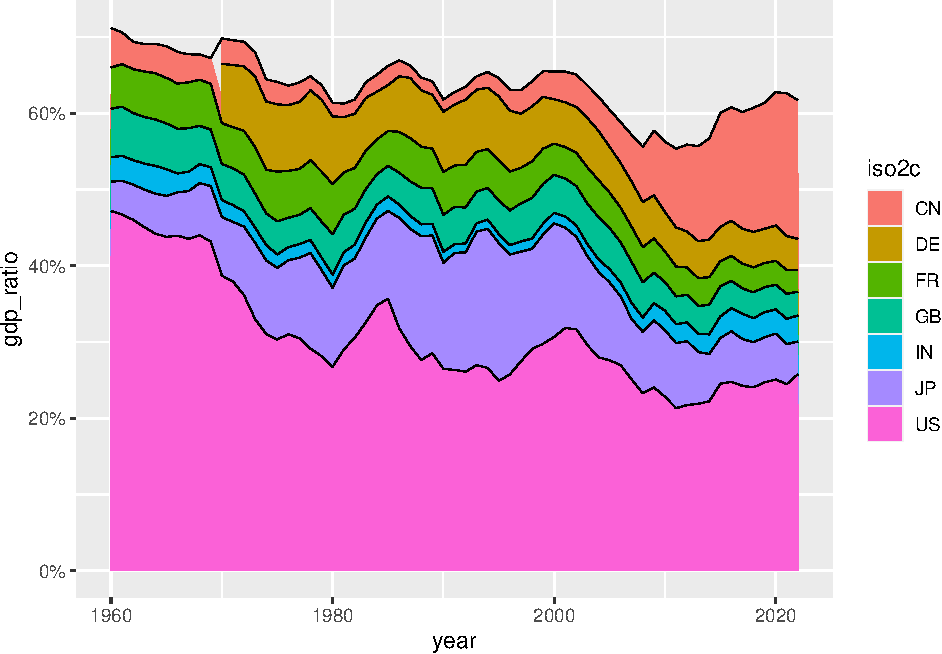
\includegraphics{41-eda_files/figure-latex/unnamed-chunk-15-1.pdf}

簡単な線形回帰モデルでの、回帰直線の y-切片や、傾きは、次のコードで与えられ、p-value や、R squared の値も求められる。

この例では、年とともに、増加の傾向があること。そして、線形モデルが\$\$、90\% 程度説明していると表現される。すなわち、

は、良い、近似であることがわかる。

\begin{Shaded}
\begin{Highlighting}[]
\NormalTok{df\_wdi\_gdppcap\_small\_short }\SpecialCharTok{\%\textgreater{}\%} \FunctionTok{lm}\NormalTok{(gdp\_pcap }\SpecialCharTok{\textasciitilde{}}\NormalTok{ year, .) }\SpecialCharTok{\%\textgreater{}\%} \FunctionTok{summary}\NormalTok{()}
\CommentTok{\#\textgreater{} }
\CommentTok{\#\textgreater{} Call:}
\CommentTok{\#\textgreater{} lm(formula = gdp\_pcap \textasciitilde{} year, data = .)}
\CommentTok{\#\textgreater{} }
\CommentTok{\#\textgreater{} Residuals:}
\CommentTok{\#\textgreater{}      Min       1Q   Median       3Q      Max }
\CommentTok{\#\textgreater{} {-}14156.8  {-}3200.5   {-}507.4   3237.7  16779.2 }
\CommentTok{\#\textgreater{} }
\CommentTok{\#\textgreater{} Coefficients:}
\CommentTok{\#\textgreater{}               Estimate Std. Error t value Pr(\textgreater{}|t|)    }
\CommentTok{\#\textgreater{} (Intercept) {-}1903497.5    48007.9  {-}39.65   \textless{}2e{-}16 ***}
\CommentTok{\#\textgreater{} year             968.3       24.1   40.18   \textless{}2e{-}16 ***}
\CommentTok{\#\textgreater{} {-}{-}{-}}
\CommentTok{\#\textgreater{} Signif. codes:  }
\CommentTok{\#\textgreater{} 0 \textquotesingle{}***\textquotesingle{} 0.001 \textquotesingle{}**\textquotesingle{} 0.01 \textquotesingle{}*\textquotesingle{} 0.05 \textquotesingle{}.\textquotesingle{} 0.1 \textquotesingle{} \textquotesingle{} 1}
\CommentTok{\#\textgreater{} }
\CommentTok{\#\textgreater{} Residual standard error: 5514 on 174 degrees of freedom}
\CommentTok{\#\textgreater{}   (10 observations deleted due to missingness)}
\CommentTok{\#\textgreater{} Multiple R{-}squared:  0.9027, Adjusted R{-}squared:  0.9021 }
\CommentTok{\#\textgreater{} F{-}statistic:  1614 on 1 and 174 DF,  p{-}value: \textless{} 2.2e{-}16}
\end{Highlighting}
\end{Shaded}

\hypertarget{part-part-v-examples}{%
\part*{(PART) PART V EXAMPLES}\label{part-part-v-examples}}
\addcontentsline{toc}{part}{(PART) PART V EXAMPLES}

\hypertarget{example1}{%
\part{Example 1}\label{example1}}

\hypertarget{appendix-appendix}{%
\part*{(APPENDIX) APPENDIX}\label{appendix-appendix}}
\addcontentsline{toc}{part}{(APPENDIX) APPENDIX}

\hypertarget{japanese}{%
\part{日本語の扱いについて}\label{japanese}}

\hypertarget{ux65e5ux672cux8a9eux4e2dux56fdux8a9eux97d3ux56fdux8a9e}{%
\chapter{日本語・中国語・韓国語}\label{ux65e5ux672cux8a9eux4e2dux56fdux8a9eux97d3ux56fdux8a9e}}

文字化けが、起こることが多く、対応が、一定せず、特に、図の表示において、Windows や、macOS や、Linux などの、OS ごとに、フォントが違ったり、それを、図のタイトルなどに、使ったりが、難しかったのですが、どうやら、現在は、どの場合も、次の設定で、解決しているようです。下の例を確認してください。特に、フォントについては、好みも関係しますから、難しいですが、ここでは、どのプラットフォーム(OS)でも、共通に扱えることを中心に書きます。

\begin{Shaded}
\begin{Highlighting}[]
\CommentTok{\# showtext を、インストールしていない場合は、一回だけ、右上の三角をクリックして実行}
\FunctionTok{install.packages}\NormalTok{(}\StringTok{\textquotesingle{}showtext\textquotesingle{}}\NormalTok{)}
\end{Highlighting}
\end{Shaded}

\hypertarget{ux30d1ux30c3ux30b1ux30fcux30b8ux3092ux30edux30fcux30c9}{%
\section{パッケージをロード}\label{ux30d1ux30c3ux30b1ux30fcux30b8ux3092ux30edux30fcux30c9}}

\texttt{library} によって、Package をロード(いつでも使えるように)します。

\begin{Shaded}
\begin{Highlighting}[]
\FunctionTok{library}\NormalTok{(tidyverse)}
\FunctionTok{library}\NormalTok{(showtext) }
\FunctionTok{showtext\_auto}\NormalTok{()}
\end{Highlighting}
\end{Shaded}

\hypertarget{base-r-ux3067ux30bfux30a4ux30c8ux30ebux306bux65e5ux672cux8a9e}{%
\chapter{Base R でタイトルに日本語}\label{base-r-ux3067ux30bfux30a4ux30c8ux30ebux306bux65e5ux672cux8a9e}}

\begin{Shaded}
\begin{Highlighting}[]
\FunctionTok{plot}\NormalTok{(cars, }\AttributeTok{main=}\StringTok{"散布図"}\NormalTok{)}
\end{Highlighting}
\end{Shaded}

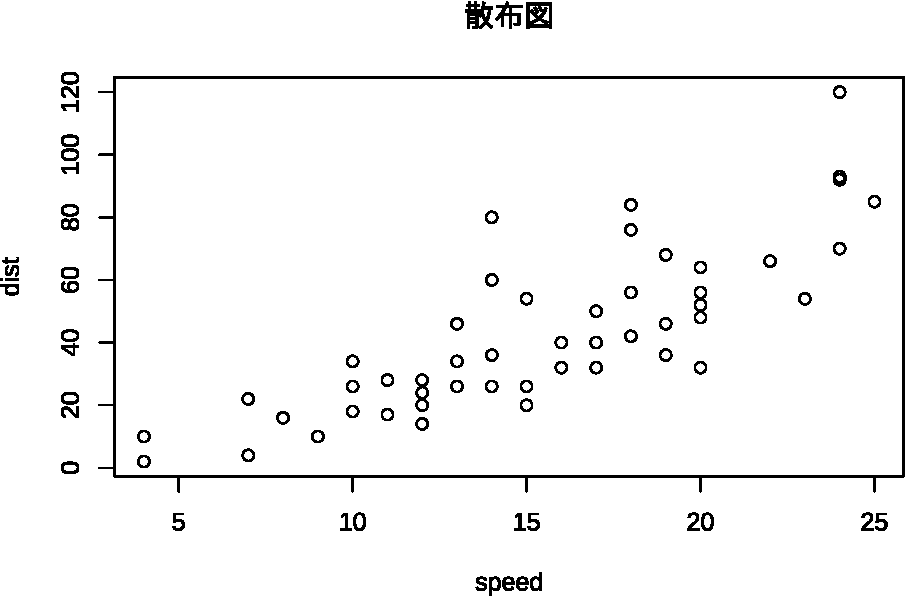
\includegraphics{81-japanese_files/figure-latex/unnamed-chunk-3-1.pdf}

\hypertarget{ux5217ux540dux3084ux30c7ux30fcux30bfux306bux65e5ux672cux8a9e}{%
\chapter{列名や、データに日本語}\label{ux5217ux540dux3084ux30c7ux30fcux30bfux306bux65e5ux672cux8a9e}}

\begin{Shaded}
\begin{Highlighting}[]
\NormalTok{df\_iris }\OtherTok{\textless{}{-}}\NormalTok{ iris}
\FunctionTok{colnames}\NormalTok{(df\_iris) }\OtherTok{\textless{}{-}} \FunctionTok{c}\NormalTok{(}\StringTok{"萼長"}\NormalTok{,}\StringTok{"萼幅"}\NormalTok{,}\StringTok{"葉長"}\NormalTok{,}\StringTok{"葉幅"}\NormalTok{,}\StringTok{"Species"}\NormalTok{ )}
\NormalTok{tab }\OtherTok{\textless{}{-}} \FunctionTok{data.frame}\NormalTok{(}\AttributeTok{Species =} \FunctionTok{c}\NormalTok{(}\StringTok{"setosa"}\NormalTok{, }\StringTok{"versicolor"}\NormalTok{, }\StringTok{"virginica"}\NormalTok{), }
                  \StringTok{"種別"} \OtherTok{=} \FunctionTok{c}\NormalTok{(}\StringTok{"ヒオウギアヤメ"}\NormalTok{, }\StringTok{"ブルーフラッグ"}\NormalTok{, }\StringTok{"バージニカ"}\NormalTok{))}
\NormalTok{df\_iris }\OtherTok{\textless{}{-}}\NormalTok{ df\_iris }\SpecialCharTok{\%\textgreater{}\%} \FunctionTok{left\_join}\NormalTok{(tab, }\AttributeTok{by=}\FunctionTok{c}\NormalTok{(}\StringTok{"Species"} \OtherTok{=} \StringTok{"Species"}\NormalTok{)) }\SpecialCharTok{\%\textgreater{}\%} \FunctionTok{select}\NormalTok{(}\SpecialCharTok{{-}}\DecValTok{5}\NormalTok{)}
\NormalTok{df\_iris }\SpecialCharTok{\%\textgreater{}\%} \FunctionTok{slice}\NormalTok{(}\DecValTok{1}\SpecialCharTok{:}\DecValTok{2}\NormalTok{)}
\CommentTok{\#\textgreater{}   萼長 萼幅 葉長 葉幅           種別}
\CommentTok{\#\textgreater{} 1  5.1  3.5  1.4  0.2 ヒオウギアヤメ}
\CommentTok{\#\textgreater{} 2  4.9  3.0  1.4  0.2 ヒオウギアヤメ}
\end{Highlighting}
\end{Shaded}

\hypertarget{kable-ux3067ux8868ux793a}{%
\chapter{\texorpdfstring{\texttt{kable} で表示}{kable で表示}}\label{kable-ux3067ux8868ux793a}}

\begin{Shaded}
\begin{Highlighting}[]
\NormalTok{knitr}\SpecialCharTok{::}\FunctionTok{kable}\NormalTok{(df\_iris[}\DecValTok{1}\SpecialCharTok{:}\DecValTok{6}\NormalTok{, ])}
\end{Highlighting}
\end{Shaded}

\begin{tabular}{r|r|r|r|l}
\hline
萼長 & 萼幅 & 葉長 & 葉幅 & 種別\\
\hline
5.1 & 3.5 & 1.4 & 0.2 & ヒオウギアヤメ\\
\hline
4.9 & 3.0 & 1.4 & 0.2 & ヒオウギアヤメ\\
\hline
4.7 & 3.2 & 1.3 & 0.2 & ヒオウギアヤメ\\
\hline
4.6 & 3.1 & 1.5 & 0.2 & ヒオウギアヤメ\\
\hline
5.0 & 3.6 & 1.4 & 0.2 & ヒオウギアヤメ\\
\hline
5.4 & 3.9 & 1.7 & 0.4 & ヒオウギアヤメ\\
\hline
\end{tabular}

\hypertarget{ggplot-ux3067ux30b0ux30e9ux30d5ux3092ux4f5cux6210}{%
\chapter{\texorpdfstring{\texttt{ggplot} でグラフを作成}{ggplot でグラフを作成}}\label{ggplot-ux3067ux30b0ux30e9ux30d5ux3092ux4f5cux6210}}

\begin{Shaded}
\begin{Highlighting}[]
\FunctionTok{ggplot}\NormalTok{(df\_iris, }\FunctionTok{aes}\NormalTok{(}\AttributeTok{x =} \StringTok{\textasciigrave{}}\AttributeTok{葉長}\StringTok{\textasciigrave{}}\NormalTok{, }\AttributeTok{y =} \StringTok{\textasciigrave{}}\AttributeTok{葉幅}\StringTok{\textasciigrave{}}\NormalTok{, }\AttributeTok{col =} \StringTok{\textasciigrave{}}\AttributeTok{種別}\StringTok{\textasciigrave{}}\NormalTok{)) }\SpecialCharTok{+}
  \FunctionTok{geom\_point}\NormalTok{() }\SpecialCharTok{+} \FunctionTok{labs}\NormalTok{(}\AttributeTok{title =} \StringTok{"散布図"}\NormalTok{, }\AttributeTok{x =} \StringTok{"葉長"}\NormalTok{, }\AttributeTok{y =} \StringTok{"葉幅"}\NormalTok{)}
\end{Highlighting}
\end{Shaded}

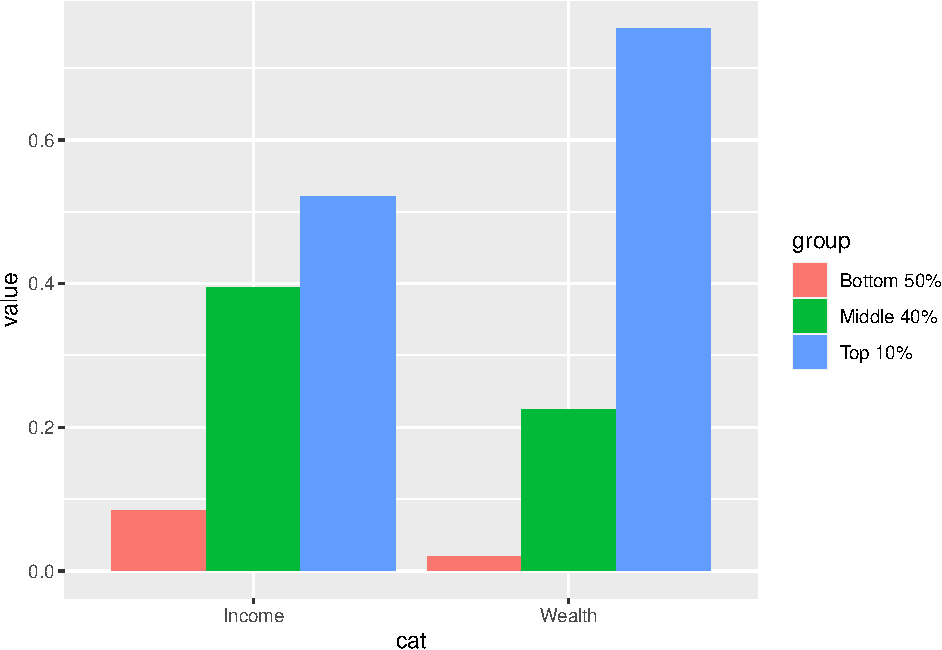
\includegraphics{81-japanese_files/figure-latex/unnamed-chunk-5-1.pdf}

\hypertarget{ux5099ux8003-1}{%
\chapter{備考:}\label{ux5099ux8003-1}}

実は、一番難しいのが、PDF の作成だと思いますが、一応、上のものも、PDF を作成することが可能です。 下のリンクのファイルを、いろいろな、形式で、出力してみてください。R Notebook と、PDF に出力したもののリンクを付けておきます。

\begin{itemize}
\tightlist
\item
  \href{https://ds-sl.github.io/intro2r/Rmarkdown-J.nb.html}{R Notebook}

  \begin{itemize}
  \tightlist
  \item
    右上の Code ボタンから、Rmd ファイルも取得できます。
  \end{itemize}
\item
  \href{https://ds-sl.github.io/intro2r/Rmarkdown-J.html}{R Notebook RMD}

  \begin{itemize}
  \tightlist
  \item
    Rmd の中身がテキストで表示されますから、コピーして、新規作成した、RNotebook ファイルに貼り付けることも可能です。
  \end{itemize}
\item
  \href{https://ds-sl.github.io/intro2r/Rmarkdown-J.pdf}{PDF}

  \begin{itemize}
  \tightlist
  \item
    通常のPDFも、やはり PDF 形式の、beamer presentation も作成できます。
  \end{itemize}
\end{itemize}

詳細は、これらのファイルに記載されていますから、参考にしてください。

\hypertarget{ux53c2ux8003ux65e5ux672cux8a9eux306eux8868ux793aux306bux3064ux3044ux3066}{%
\chapter{参考:日本語の表示について}\label{ux53c2ux8003ux65e5ux672cux8a9eux306eux8868ux793aux306bux3064ux3044ux3066}}

\begin{quote}
日本語が適切に表示されない!?
\end{quote}

簡単ではなく、未解決の部分が何かなどを含め、わたしも十分理解できているか不明であるが、理解できていると思われる範囲で、備忘録のように記します。

R を使うという場合に限っても、R Studio IDE を使う場合、RStudio Cloud を使う場合、Google colab を使う場合、他のプラットフォームで使う場合で違ってくると思われますが、上にあげた、三種類のプラットフォームで確かめられるものについて書いていく。上に書いた以外に、R Studio IDE を、Windows 上で使う場合と、Mac 上で使う場合(Mac のシステムは Unix 系であるが、さまざまな Linux )でも、状況が異なるかもしれません。そこで、場合分けをして書いていくほうが安全ですが、それは、極力避け、どれにでも適用可能な方法を模索しながら書いていこうと思います。個人的に、日常的に分断を避ける努力をすることが大切だと思っていることも背景にある。さらに、ソフトウェア開発者は、むろん、そのような差異を理解して、どの環境でも、可能なように設計することを心がけていると思われますし、そのようなものが、R Project の正規のパッケージとして採用されていくべきだとも考えていますので、多少、理想も入っているが、これを基本として書いていこうと思います。十分なチェックができていないものもあるので、不具合などは、ぜひ、お知らせ願いたい。この文章も少しずつ、改善していければと思う。

通常、日本語、中国語、韓国語などが適切に表示できない場合は、文字のエンコーディング(Encoding: どのような情報として記録されているか)と、フォントの問題、さらに、システムがこれらをどう処理しているかの問題があると思われます。しかし、R の利用者として考えると、文字化けが起きたり、適切に文字が表示されないのは、以下の三つに分けられるようです。

\begin{enumerate}
\def\labelenumi{\arabic{enumi}.}
\tightlist
\item
  データファイルなどを読み込んだときに適切に表示されない
\item
  図の中のタイトルなどが、適切に表示されない
\item
  R Markdown の出力において、適切に表示されない
\end{enumerate}

\hypertarget{ux30c7ux30fcux30bfux30d5ux30a1ux30a4ux30ebux306eux8aadux307fux8fbcux307f}{%
\section{データファイルの読み込み}\label{ux30c7ux30fcux30bfux30d5ux30a1ux30a4ux30ebux306eux8aadux307fux8fbcux307f}}

\begin{itemize}
\tightlist
\item
  tidyverse に含まれる readr には、guess\_encoding が含まれており、一般的には、たとえば、

  \begin{itemize}
  \tightlist
  \item
    read\_csv(``./data/file\_name.csv'') とすると、一番可能性の高いエンコーディングで読み込まれるようになっています。
  \end{itemize}
\item
  使い方:guess\_encoding(file, n\_max = 10000, threshold = 0.2) とあり、10000行で推測されたエンコーディング、または、確率を計算することを 初期設定値(Default)にしてます。Help によると、すべての行をチェックする場合は、n\_max = -1 とすることが書かれています。
\item
  これで問題がない場合が多いです。他の、readr 関数も同様です。しかし、これは、あくまでも、CSV などのテキストファイルについてです。
\item
  なお、read\_csv などにも、guess\_max = min(1000, n\_max) もありますが、これは、column type を決めるためのものである。
\item
  read.csv() など、base R では、fileEncoding = ````, encoding =''unknown'' がオプションに含まれていたので、指定して読み込むことが通常でした。
\end{itemize}

\hypertarget{ux56f3ux306eux4e2dux306eux30c6ux30adux30b9ux30c8}{%
\section{図の中のテキスト}\label{ux56f3ux306eux4e2dux306eux30c6ux30adux30b9ux30c8}}

\begin{itemize}
\tightlist
\item
  基本的には、日本語を表示できるフォントがインストールされていて、図の表示の前にlibrary(showtext); showtext\_auto() となっていれば、これ以降の図は、問題なく、表示されるはずです。
\item
  通常使っている、コンピュータ以外で、使うときに、フォントが入っていない場合などは、\texttt{tinytex} の命令を使って、\texttt{tinytex::tlmgr\_install("ipaex")} とすれば、PDF を作成するときも、IPA フォント(International Phonetic Alphabet)を使えます。
\item
  二種類以上のフォントを使い分けたいときは、名前をつけて、それを family = name で指定する。

  \begin{itemize}
  \tightlist
  \item
    showtext: Using Fonts More Easily in R Graphs 参照。
  \end{itemize}
\end{itemize}

\hypertarget{r-markdown-ux306eux51faux529b}{%
\section{R Markdown の出力}\label{r-markdown-ux306eux51faux529b}}

\begin{itemize}
\tightlist
\item
  PDF 作成には、\TeX システムを使っているので、日本語を扱えるように、tex-engine や、document class や、mainfont を設定する必要があるが、R Markdown ファイルの YAML に、以下を加えれば問題がないようである。
\end{itemize}

\begin{verbatim}
header-includes:
  - \usepackage{xeCJK}
  - \setCJKmainfont{ipaexm.ttf}
  - \setCJKsansfont{ipaexg.ttf}
  - \setCJKmonofont{ipaexg.ttf}
\end{verbatim}

\hypertarget{bookdown}{%
\section{\texorpdfstring{\texttt{bookdown}}{bookdown}}\label{bookdown}}

\texttt{bookdown} を使って、電子書籍を出版する場合には、\href{https://bookdown.org/yihui/bookdown/}{\texttt{bookdown} (リンク)} を参照してください。

日本語におけるテンプレートは、\href{https://github.com/icu-hsuzuki/bs4_book_template}{こちら} にあります。まずは、ページの下にある、README を読んでください。

\hypertarget{ux53c2ux8003ux3068ux3057ux305fux3082ux306e}{%
\section{参考としたもの}\label{ux53c2ux8003ux3068ux3057ux305fux3082ux306e}}

\hypertarget{showtext-using-fonts-more-easily-in-r-graphs}{%
\subsection{showtext: Using Fonts More Easily in R Graphs}\label{showtext-using-fonts-more-easily-in-r-graphs}}

\begin{itemize}
\tightlist
\item
  \url{https://CRAN.R-project.org/package=showtext}

  \begin{itemize}
  \tightlist
  \item
    \url{https://cran.r-project.org/web/packages/showtext/readme/README.html}
  \item
    showtext: Using Fonts More Easily in R Graphs:

    \begin{itemize}
    \tightlist
    \item
      \url{https://cran.r-project.org/web/packages/showtext/vignettes/introduction.html}
    \item
      \url{https://fonts.google.com}
    \end{itemize}
  \end{itemize}
\end{itemize}

\hypertarget{sysfonts-loading-fonts-into-r}{%
\subsection{sysfonts: Loading Fonts into R}\label{sysfonts-loading-fonts-into-r}}

\begin{itemize}
\tightlist
\item
  \url{https://CRAN.R-project.org/package=sysfonts}

  \begin{itemize}
  \tightlist
  \item
    \url{https://cran.r-project.org/web/packages/sysfonts/sysfonts.pdf}
  \end{itemize}
\end{itemize}

\hypertarget{foods4all-examples-of-graphs}{%
\subsection{foods4all: Examples of Graphs}\label{foods4all-examples-of-graphs}}

\begin{itemize}
\tightlist
\item
  \url{https://foods4all.github.io/examples/examples_of_graphs.html}

  \begin{itemize}
  \tightlist
  \item
    77.2 Japanese Environments 日本語環境(昔の記事:Last Updated: 2020-04-22)
  \end{itemize}
\end{itemize}

\hypertarget{tools}{%
\part{IT ツール}\label{tools}}

\begin{quote}
いくつかの便利なツールについて紹介します。
\end{quote}

\hypertarget{git-ux3068-github}{%
\chapter{Git と GitHub}\label{git-ux3068-github}}

Git は バージョン管理システムで、GitHub はそれを、活用し、かつ他のメンバーと協力して開発など、さまざまな活動をするためのサイトです。公開が基本となっています。非公開にすることも可能ですが、公開することで、世界中のひとたちと協力していくことが可能になりますので、その利点も学んでいただければと思います。

\hypertarget{ux6982ux8981}{%
\section{概要}\label{ux6982ux8981}}

RStudio で R を使っている場合、Git-GitHub-RStudio の連携で使うことをお勧めします。しかし、これらは、三つとも、まったく異なるものですから、簡単な概要を書いておくことにします。

\hypertarget{git}{%
\subsection{Git}\label{git}}

これは、ファイルのバージョン(更新履歴)の管理システムで、単独で機能します。他の、プログラムなどに関係しない、他の文書ファイルであっても、バージョンを管理する場合に活用できます。特に、テキスト・ファイルの場合には、どこがどう改訂されているかを確認することもできます。また、基本的には、Unix の Shell プログラムで動作させるのが一般的です。Mac は、Unix システムの上に構築されているため、最初から、ユーティリティ(Utility)\textgreater{} ターミナル(Terminal)で、Shell コマンドが利用可能になっていますが、Windows の場合には、bash と呼ばれる Shell プログラムをインストールすることをお勧めします。Windows システムについてよくご存知の方は、他の方法を使っていただいて構いませんが、Git のインストールの時に、Git bash を選択して、簡単に インストールできますし、Unix システムの基本を理解するチャンスでもあり、Mac とも同じ環境で説明できますから、ここでは、そちらを使います。Shell コマンドは、R Studio の中のターミナルを使って、利用することも可能です。(注:Windows のコマンド・プロンプト、または、パワー・シェルをお使いの方は、利用環境が変化する可能性がありますから、そのまま使われる方が良いかもしれません。)

基本的なコマンドとしては、以下のものがあります。いまは、このようなものがある程度に、眺めておいてください。

\begin{itemize}
\tightlist
\item
  \texttt{git\ init}: 特定のディレクトリ(フォルダ)で バージョン管理を始める時に使います。
\item
  \texttt{git\ status}: 現在の状況を確認するときに使います。
\item
  \texttt{git\ diff\ file\_name}: ファイルへの変更を確認します。
\item
  \texttt{git\ log}: 過去の commit による履歴を確認する時に使います。
\item
  \texttt{git\ add\ file\_name}: ステージングという中間的な場所に登録します。
\item
  \texttt{git\ commit\ -m\ "log\ message\ here"}: ステージングにあるものを、確定させます。引用符で囲まれた短いコメントを加えます。50文字が上限です。
\item
  \texttt{git\ help}: Help のリストが表示されます。

  \begin{itemize}
  \tightlist
  \item
    例:\texttt{git\ help\ init} などと入力すると、説明を見ることができます。
  \end{itemize}
\end{itemize}

\hypertarget{git-hub}{%
\subsection{Git Hub}\label{git-hub}}

Git でバージョン管理されているディレクトリ(フォルダ)の状態を示す、クラウドサービスです。更新されている、状態を確認するとともに、変更履歴なども確認できます。また、Git Hub サービスを利用して、ファイルを公開、共有することも可能です。Pages サイトを利用することで、ホームページとして HTML ファイルなどを公開することもできるため、レポートを公開したり、この電子書籍のように、\texttt{bookdown} パッケージを利用して作成したものを、インターネット上に公開することも可能です。

お気付きかと思いますが、この電子書籍も、リンクされている、他の文書も、URL(アドレス)をみると、GitHub になっていますし、パッケージや、データなども、GitHub へのリンクが示されている割合が、非常に高いと思います。

最初に、Git で管理されている、ディレクトリ(フォルダ)(これを、ローカル・リポジトリと言います)と、GitHub 内のリポジトリ(リモート・リポジトリまはたアップストリーム・リポジトリと言います。ここでは、リモート・リポジトリと呼ぶことにします)を結びつけるステップが必要です。

\hypertarget{rstudio-ux9023ux643a}{%
\subsection{RStudio 連携}\label{rstudio-ux9023ux643a}}

コマンドライン(シェル)で行う作業や、ローカル・リポジトリを、リモート・リポジトリに結びつける作業を、RStudio の中で行うことが可能です。

\hypertarget{ux306fux3058ux3081ux304bux305f}{%
\section{はじめかた}\label{ux306fux3058ux3081ux304bux305f}}

\begin{enumerate}
\def\labelenumi{\arabic{enumi}.}
\tightlist
\item
  Git のインストール
\end{enumerate}

\begin{itemize}
\tightlist
\item
  Windows と Mac で異なりますので注意が必要です。Mac については、\textbf{Mac} と書いてあるところを読んでください。
\item
  \textbf{Windows} の場合は、\href{https://git-scm.com/download/win}{git-scm} にアクセスしてダウンロード、インストールしてください。セットアップ(Setup)で、2箇所、注意点があります、それ以外は、すべて、初期設定のままで変更は必要ありません。

  \begin{itemize}
  \tightlist
  \item
    Choosing the default editor used by Git: 設定で、エディタ(Editor)を設定しますが、vi, vim に慣れていない方は、nano を選択することをお勧めします。(nano\footnote{GNU nanoは、コンソールウィンドウで動作する小型でフレンドリーなテキストエディタです。(GNU nano is a small and friendly text editor running in the console window.)} は、メニューが下に出るので、それを見て操作することが可能なエディターです。)
  \item
    Adjusting Your Path Environment: Windows の コマンドライン・ツール(command line prompt) を使っていない方は、Git Bash のインストールを選択してください。さらに、Git and optional Unix tools from the Windows Command Prompt を選択することをお勧めしますが、上で書いたように、Windows の コマンド・プロンプトになれておられる方で、それを使い続けたいかたは、Use Git from Git Bash only を選択されるのが良いかもしれません。
  \item
    最後に、RStudio の設定(Tools \textgreater{} Global Option)で、Terminal から、Git Bash を選択\footnote{自動的に選択されているかもしれません}し、Tools から、New Terminal を選択\footnote{すでにタブがあればこの作業は不要です}します。
  \end{itemize}
\item
  \textbf{Mac} は、最初から、Install されていると思います。ユーティリティ(Utility)\textgreater{} ターミナル(Terminal)を開いて\footnote{RStudio を既にお使いの方は、左下の窓枠から、Terminal タブを選択できますので、それを使うことも可能です。}、\texttt{git\ -\/-version} とすると、インストールされているバージョンが表示されると思います。バージョンがでない場合には、Install するかと聞かれます。このときに、Git だけをインストールすることも、Xcode という開発環境を同時にインストールすることも可能です。(インストールするように指示が出なければ、App Store からも、インストールできます。もし、そのあとで、git などのコマンドで xcrun: error などとエラーが出たら、\texttt{xcode-select\ -\/-install} としてください。)インストールが終了したら、もう一度、\texttt{git\ -\/-version} と Terminal に入力して、結果を確認してください。
\end{itemize}

ぎt2. GitHub のアカウント取得 - \href{https://github.com}{GitHub サイト} に、アカウントを作成します。アカウント名は、短く、分かりやすく、覚えやすいものをよく考えて決めてください。Email Address だけで、無償で作成できます。

\begin{enumerate}
\def\labelenumi{\arabic{enumi}.}
\setcounter{enumi}{2}
\tightlist
\item
  RStudio の 左下の窓枠のTerminal タブ\footnote{Terminal がない場合は、Tools \textgreater{} Terminal \textgreater{} New Terminal とすると表示されます。}から、GitHub アカウントに連携する設定を行います。 下の2行を、1行ずつ、コピーして、Terminal に入力してください。
\end{enumerate}

\begin{verbatim}
git config --global user.name "Your Name" # GitHub の User Name
git config --global user.email "your@email.com" # GitHub に登録したメールアドレス
\end{verbatim}

\begin{enumerate}
\def\labelenumi{\arabic{enumi}.}
\setcounter{enumi}{3}
\tightlist
\item
  RStudio の、Tools \textgreater{} Global Opton の、Git/SVN タブを開き、Git Executable とあるところに、Git 実行プログラムのある場所を入れます。
\end{enumerate}

\begin{itemize}
\tightlist
\item
  \textbf{Windows} の場合は、\texttt{C:/Program\ Files/Git/bin/git.exe} だと思いますが、Browse ボタンから確認してください。
\item
  \textbf{Mac} の場合は、\texttt{/usr/bin/git} になるかと思いますが、Browse ボタンから確認してください。
\end{itemize}

\begin{enumerate}
\def\labelenumi{\arabic{enumi}.}
\setcounter{enumi}{4}
\item
  その下に、Create RSA key とありますから、それを押し、Create ボタンを押しててください\footnote{Passphrase (optional) と出ますが、無視してくださって構いません。}。すると、View RSA key から、暗号キーも確認できます。(この作業は、Terminal から、\texttt{ssh-keygen\ -t\ rsa} として作成することも可能です。この作業で、\texttt{\textasciitilde{}/.ssh/} 内に、SSH キーが記述されたファイルが作成されます。)
\item
  GitHub アカウントで公開鍵を利用できるようにします。まず、RStudio の方で作成した、RSA key (Tools の、Global Option の Git/SVN)の下にある view を押すと見ることができ、上に、書いてあるように、そこに出てきたものを、コピーします。次に、GitHubにログインし、右上のアイコンの右の三角から、設定(Setting)を選択し、SSH公開鍵(SSH and GPG Keys)を選択します。新しい公開鍵を追加(New SSH Key)を選択すると、SSH キーを貼り付けることができます。(リポジトリの左上にある、アカウント名をクリックし現れるダッシュボードの左上の大きなアイコンをクリックしても「アカウント設定」が現れ、SSH and GPG Keysを見つけることができると思います。)
\end{enumerate}

(なお、RStudio ではなく、Terminal からコピーするときは、Unix では、\texttt{pbcopy\ \textless{}\ \textasciitilde{}/.ssh/id\_rsa.pub} などとします。Windows の場合は、\texttt{pbcopy} が使えない可能性があるので、そのときは、Terminal から、Git Bash を使い、\texttt{use\ \textless{}\ \textasciitilde{}/.ssh/id\_rsa.pub} とします。Terminal に慣れておられない方には、上に紹介した、RStudio からコピーする方が簡便かと思います。)

\begin{enumerate}
\def\labelenumi{\arabic{enumi}.}
\setcounter{enumi}{6}
\tightlist
\item
  これで設定終了ですので、R Studio を再起動させてください。
\end{enumerate}

\hypertarget{github-ux306bux3042ux308bux30eaux30e2ux30fcux30c8ux30eaux30ddux30b8ux30c8ux30earemote-repoux304bux3089ux59cbux3081ux308bux5834ux5408}{%
\section{GitHub にあるリモート・リポジトリ(Remote Repo)から始める場合}\label{github-ux306bux3042ux308bux30eaux30e2ux30fcux30c8ux30eaux30ddux30b8ux30c8ux30earemote-repoux304bux3089ux59cbux3081ux308bux5834ux5408}}

\begin{enumerate}
\def\labelenumi{\arabic{enumi}.}
\tightlist
\item
  GitHub にログインして、既存のリポジトリを開きます。
\item
  Code の、Clone から、リンク先のアドレスを入手。https と SSH を選べますが、SSH を選び、コピーします。
\item
  RStudio から、New Project とし、Version Control を選択し、ディレクトリーを決めたら、上でコピーした、ものを、貼り付けて、Project を作成します。
\end{enumerate}

この手続きで、リモート・リポジトリのファイルがすべて、RStudio のプロジェクトに入ります。

実はこの手続きで、公開されている、他のリポジトリも取り込むことができます。ただし、編集して、改訂していくには、自分のリポジトリに、繋ぐことになります。そのときは、次の項目を見てください。

\hypertarget{ux81eaux5206ux306eux30b3ux30f3ux30d4ux30e5ux30fcux30bfux306eux30eaux30ddux30b8ux30c8ux30ealocal-repoux304bux3089ux59cbux3081ux308bux5834ux5408}{%
\section{自分のコンピュータのリポジトリ(Local Repo)から始める場合}\label{ux81eaux5206ux306eux30b3ux30f3ux30d4ux30e5ux30fcux30bfux306eux30eaux30ddux30b8ux30c8ux30ealocal-repoux304bux3089ux59cbux3081ux308bux5834ux5408}}

\begin{enumerate}
\def\labelenumi{\arabic{enumi}.}
\tightlist
\item
  RStudio から新しい、プロジェクト(Project) を作成 \texttt{test0} としておきましょう。
\item
  GitHub に、新しい、レポジトリを作成して繋げる
\end{enumerate}

\begin{itemize}
\tightlist
\item
  自分の GitHub アカウントに、新しい、レポジトリをプロジェクトと同じ名前 \texttt{test0} で作成します。同じ名前でなくてもかまわないのですが、関連がしやすいので、同じ名前がお勧めです。
\item
  Quick Setup というページが表示されますから、その、下の Set up in Desktop or の右から、https と SSH を選べますが、SSH を選び、コピーします。
\item
  プロジェクトの中の 左下の窓枠の、Terminal から次を実行します。
\end{itemize}

\begin{verbatim}
echo "# Project test0" >> README.md # REAME の表題を書きます。
git init
git add README.md
git commit -m "First commit. README.md"
git branch -M main
git remote add origin `git@github.com:icu-hsuzuki/test0.git`
# わたしのアカウントの場合には、コピーしたものを貼り付けると、上のようになります。
git push -u origin main
\end{verbatim}

再起動すると、プロジェクトの右上の窓枠に、Git と表示されていると思います。開いて、いくつかファイル名があれば、これを選択し、Commit ボタンを押し、短い message を書いて、Commit とし、そのあとで、Push ボタンを押してください。 \texttt{HEAD\ -\textgreater{}\ main} と表示されれば、OK です。

\hypertarget{github-pages-ux306bux3064ux3044ux3066}{%
\section{GitHub Pages について}\label{github-pages-ux306bux3064ux3044ux3066}}

GitHub は、Web 上のサービスですが、たとえ、リポジトリーの中に、HTML ファイルなどが存在しても、ブラウザーで表示させることはできません。公開する方法として、わたしは、以下のようにしています。

公開しブラウザーで読めるようにしたいファイルを、\texttt{docs} という ディレクトリに入れます。Setting を選択し、左の帯から、Pages を選び、Branch を、\texttt{main}、\texttt{/docs} として、Save します。すると、docs に入っているファイルは、リンクを指定すれば、ブラウザーで、見ることができます。

リンクは、まず、リポジトリーの右上の、About の右のギアマークから、Use your GitHub Pages website に、チェックを入れると、URL が表示されますから、その URL に続けて、ファイル名を加えたものが、そのファイルの、リンクとなります。

\hypertarget{bookdown-ux30d1ux30c3ux30b1ux30fcux30b8ux306bux3088ux308bux96fbux5b50ux66f8ux7c4dux306eux57f7ux7b46}{%
\section{Bookdown パッケージによる、電子書籍の執筆}\label{bookdown-ux30d1ux30c3ux30b1ux30fcux30b8ux306bux3088ux308bux96fbux5b50ux66f8ux7c4dux306eux57f7ux7b46}}

\href{https://github.com/rstudio/bookdown}{bookdown} を利用して、始める方法を簡単に記します。

Git-GitHub-RStuio の設定は済んでいると仮定して書きます。また、Bookdown を利用するには、\texttt{bookdown} パッケージのインストールが必要です。RStudio の Tools から、Install Packages を選択して、インストールしてください。また、\texttt{bs4\_book} スタイルを利用する場合は、RStudio などのバージョンによっては、\texttt{bslib} と \texttt{downlit} も、インストールする必要があるようです。

以下では、R Studio で新しい、プロジェクトとして始める場合と、テンプレート・リポジトリ を使う方法を説明します。

\hypertarget{rstudio-ux3067ux306eux8a2dux5b9a}{%
\subsection{RStudio での設定}\label{rstudio-ux3067ux306eux8a2dux5b9a}}

\begin{enumerate}
\def\labelenumi{\arabic{enumi}.}
\tightlist
\item
  新しい book プロジェクトを始めます、標準設定の \texttt{book} と、\texttt{bs4\_book} を選択できます。このディレクトリ(フォルダ。ローカル・リポジトリと呼びます)の名前をリモート・リポジトリの名前と同じにして、作成します\footnote{異なる名前でも可能ですが、特別な理由がない限り同じにしておいた方が良いでしょう}。
\item
  Files の、Rename 機能を使って \texttt{\_book} ディレクトリ(フォルダ)の名前を、\texttt{docs} に変更します。
\item
  \texttt{\_bookdown.yml} を編集し次の行を加えます(私は2行目に入れています)。\\
  \texttt{output\_dir:\ docs}\strut \\
  GitHub Pages の機能を使って、公開するための変更です。
\item
  \textbf{@GitHub:} 新いリポジトリー(リモート・リポジトリと言います)を作成します。ローカル・リポジトリと同じ名前にし、簡単な説明を加えます。
\item
  左下の窓枠から、Terminal タブを選択します。 以下は例です。\texttt{git\ remote\ add\ origin} のところは、適当に変更してください。
\end{enumerate}

\begin{verbatim}
echo "# ds-book" >> README.md
git init
git add README.md
git commit -m "first commit"
git branch -M main
git remote add origin git@github.com:icu-hsuzuki/ds4aj.git # 変更
git push -u origin main
\end{verbatim}

\begin{enumerate}
\def\labelenumi{\arabic{enumi}.}
\setcounter{enumi}{4}
\tightlist
\item
  RStudio を一旦終了し、もう一度、そのプロジェクトを立ち上げると、右上の窓枠に、Git タブが表示されるはずです。
\item
  Build から、Build Book ボタンを利用すれば、作成されます。
\item
  Git タブから: Commit ``first build'' とし、 Push をします。
\item
  \textbf{@GitHub:} Settings から、Pages \textgreater{} main \textgreater{} docs と変更すると、公開されます。
\item
  Code に戻り、About の右のギアマークから、
\end{enumerate}

\hypertarget{ux4ed6ux306e-pc-ux3067ux306eux4f5cux696d}{%
\subsubsection{他の PC での作業}\label{ux4ed6ux306e-pc-ux3067ux306eux4f5cux696d}}

\begin{enumerate}
\def\labelenumi{\arabic{enumi}.}
\tightlist
\item
  Login to GitHub account
\item
  Copy SSH address under Code\textgreater Clone
\item
  Create a new project using Version Control:Git with the SSH address by setting the directory name
\item
  Edit README.md and test Git Commit and Push
\end{enumerate}

\hypertarget{ux30c6ux30f3ux30d7ux30ecux30fcux30c8ux3092ux5229ux7528ux3059ux308bux65b9ux6cd5}{%
\subsection{テンプレートを利用する方法}\label{ux30c6ux30f3ux30d7ux30ecux30fcux30c8ux3092ux5229ux7528ux3059ux308bux65b9ux6cd5}}

\hypertarget{bookdown-demo}{%
\subsubsection{bookdown-demo}\label{bookdown-demo}}

\href{https://bookdown.org/yihui/bookdown/}{\texttt{bookdown} の電子書籍(bookdown: Authoring Books and Technical Documents with R Markdown)} の、はじめてみよう(Get started)から、GitHub リポジトリー \href{https://github.com/rstudio/bookdown-demo}{rstudio/bookdown-demo} にリンクがついています。

\begin{enumerate}
\def\labelenumi{\arabic{enumi}.}
\tightlist
\item
  自分の、GitHub アカウントに、ログインします。
\item
  \href{https://github.com/rstudio/bookdown-demo}{rstudio/bookdown-demo} にアクセスし、Use this template から、create a new repository を選択します。
\item
  自分のアカウントの中に、コピーされたリポジトリーがつくられます。
\item
  上で説明した「GitHub にあるリモート・リポジトリ(Remote Repo)から始める場合」を利用してください。
\end{enumerate}

よくできているテンプレートです。しかし、このままでは、公開されません。\href{https://bookdown.org/yihui/bookdown/}{bookdown: Authoring Books and Technical Documents with R Markdown} には、いくつかの公開方法が書かれていますから、参照してください。

\hypertarget{jtr13bookdown-template}{%
\subsubsection{\texorpdfstring{\texttt{jtr13/bookdown-template}}{jtr13/bookdown-template}}\label{jtr13bookdown-template}}

YouTube ビデオ \href{https://www.youtube.com/watch?v=m5D-yoH416Y}{5分間で、bookdown の本を作成する方法(How to create a bookdown book in 5 minutes)} で紹介されているものです。

\begin{enumerate}
\def\labelenumi{\arabic{enumi}.}
\tightlist
\item
  自分の、GitHub アカウントに、ログインします。
\item
  \href{https://github.com/jtr13/bookdown-template}{jtr13/bookdown-template} にアクセスし、Use this template から、create a new repository を選択します。
\item
  自分のアカウントの中に、コピーされたリポジトリーがつくられます。
\item
  上で説明した「GitHub にあるリモート・リポジトリ(Remote Repo)から始める場合」を利用してください。
\end{enumerate}

ビデオの中では、簡単に、GitHub Pages(GitHub のホームページサービス)に、公開する方法が説明されています。最も、大切な部分は、テンプレートがコピーされた、自分のリポジトリの Settings から、Pages を選び、Branch を main \textgreater{} docs とする部分です。このようにすることで、公開されます。上の、「GitHub Pages」で説明していることと同じです。

\hypertarget{ux65e5ux672cux8a9eux30c6ux30f3ux30d7ux30ecux30fcux30c8}{%
\subsubsection{日本語テンプレート}\label{ux65e5ux672cux8a9eux30c6ux30f3ux30d7ux30ecux30fcux30c8}}

\texttt{bs4\_book} スタイルでの、簡単な、日本語テンプレートを作成しました。

\begin{enumerate}
\def\labelenumi{\arabic{enumi}.}
\tightlist
\item
  自分の、GitHub アカウントに、ログインします。
\item
  \href{https://github.com/icu-hsuzuki/bs4_book_template}{icu-hsuzuki/bs4\_book\_template} にアクセスし、Use this template から、create a new repository を選択します。
\item
  自分のアカウントの中に、コピーされたリポジトリーがつくられます。
\item
  上で説明した「GitHub にあるリモート・リポジトリ(Remote Repo)から始める場合」を利用してください。
\end{enumerate}

まだ、不十分ですが、少しずつ、改訂していきます。 使い方は、リポジトリの README に、注意点などは、最後の章 Bookdown に書いておく予定です。

\hypertarget{ux5927ux304dux306aux30d5ux30a1ux30a4ux30ebux306bux95a2ux3059ux308bux3053ux3068}{%
\section{大きなファイルに関すること}\label{ux5927ux304dux306aux30d5ux30a1ux30a4ux30ebux306bux95a2ux3059ux308bux3053ux3068}}

100M 未満のファイルだけを利用するのがよいですが、それより大きいものを、GitHub に挙げようとして、問題が起こることがあります。その対処法を書いておきます。

個人的には、大きなデータや、本などを、Build して、100M 以上の、非常に大きな、TeX 関連のファイルができることがありました。

備忘録も含めて、書いておきます。

\hypertarget{ux5927ux304dux306aux30d5ux30a1ux30a4ux30ebux306eux53d6ux308aux9664ux304dux304bux305f}{%
\subsection{大きなファイルの取り除きかた}\label{ux5927ux304dux306aux30d5ux30a1ux30a4ux30ebux306eux53d6ux308aux9664ux304dux304bux305f}}

下のサイトからの引用です。非常に分かりやすく書かれています。Terminal で作業を行いますが、いま、Add した場合と、いくつか、前のステップで、Add した場合で、対応の方法が異なります。

\begin{itemize}
\tightlist
\item
  \href{https://medium.com/analytics-vidhya/tutorial-removing-large-files-from-git-78dbf4cf83a}{Tutorial: Removing Large Files from Git}

  \begin{itemize}
  \tightlist
  \item
    Scenario 1: The Large File Was Just Added in the Most Recent Commit

    \begin{itemize}
    \tightlist
    \item
      git rm --cached big\_file\_name
    \item
      git commit --amend -C HEAD
    \end{itemize}
  \item
    Scenario 2: The Large File Was Committed Prior to The Most Recent Commit

    \begin{itemize}
    \tightlist
    \item
      Locating the Last ``Good'' Commit: git log --oneline
    \item
      Initiate a Rebase Between the Last ``Good'' Commit and the Current Commit: git rebase -i 8464da4
    \item
      This will open up a file in your Git editor (in my case, Vim), that looks something like this:

      \begin{itemize}
      \tightlist
      \item
        pick -\textgreater{} edit
      \end{itemize}
    \item
      git rm --cached csv\_building\_damage\_assessment.csv
    \item
      git commit --amend -C HEAD
    \end{itemize}
  \end{itemize}
\end{itemize}

\hypertarget{ux8907ux6570ux306eux30b3ux30f3ux30d4ux30e5ux30fcux30bfux304bux3089ux5229ux7528ux3059ux308bux65b9ux6cd5}{%
\section{複数のコンピュータから利用する方法}\label{ux8907ux6570ux306eux30b3ux30f3ux30d4ux30e5ux30fcux30bfux304bux3089ux5229ux7528ux3059ux308bux65b9ux6cd5}}

わたしも、いくつかのコンピュータから、同じGitHub アカウントにアクセスして作業しています。

同じSSHキーを、複数のコンピュータで利用することも可能です。特に、コンピュータの更新時に、移行する場合は、元の環境をそのまま使うことも可能で便利です。

ただし、基本的には、それぞれのコンピュータで別々のSSHキーを使用するのがお勧めです。問題が発生した時に、個別のコンピュータの課題として解決することができます。

(たとえば、RSA 形式で作成した)複数の SSH キーを使用するときは、GitHub アカウントに公開鍵を追加する必要があります。

GitHub アカウントに別の公開鍵を追加するには、GitHubにログインし、右上のアイコンの右の三角から、設定(Setting)を選択し、SSH公開鍵(SSH and GPG Keys)を選択します。新しい公開鍵を追加(New SSH Key)を選択すると、SSH キーを貼り付けることができます。(リポジトリの左上にある、アカウント名をクリックし現れるダッシュボードの左上の大きなアイコンをクリックしても「アカウント設定」が現れ、SSH and GPG Keysを見つけることができると思います。)

コピーを貼り付ける時には、RStudio の、Global Option の、Git/SVN タブから、View public key を見ると、コピーできるようになっています。

Terminal からコピーするときは、Unix では、\texttt{pbcopy\ \textless{}\ \textasciitilde{}/.ssh/id\_rsa.pub} などとします。Windows の場合は、\texttt{pbcopy} が使えない可能性があるので、そのときは、Terminal から、Git Bash を使い、\texttt{use\ \textless{}\ \textasciitilde{}/.ssh/id\_rsa.pub} とします。Terminal に慣れておられない方には、上に紹介した、RStudio からコピーする方が簡便かと思います。

SSH キーの最後には、コンピュータ名とコンピュータのアカウント名などが入っていると思います。

この設定をすれば、どちらのマシンからでもSSH経由でGithubリポジトリにアクセスできるようになります。

\hypertarget{ux8907ux6570ux306eux30a2ux30abux30a6ux30f3ux30c8ux3092ux4e00ux3064ux306eux30b3ux30f3ux30d4ux30e5ux30fcux30bfux304bux3089ux5229ux7528ux3059ux308bux65b9ux6cd5}{%
\section{複数のアカウントを一つのコンピュータから利用する方法}\label{ux8907ux6570ux306eux30a2ux30abux30a6ux30f3ux30c8ux3092ux4e00ux3064ux306eux30b3ux30f3ux30d4ux30e5ux30fcux30bfux304bux3089ux5229ux7528ux3059ux308bux65b9ux6cd5}}

わたしも複数のGitHub アカウントを利用しています。

\begin{itemize}
\tightlist
\item
  \textasciitilde/.ssh 内に 複数(例では三つ)、ssh-keygen -t rsa でファイル作成

  \begin{itemize}
  \tightlist
  \item
    id\_rsa , id\_sub1\_rsa, id\_sub2\_rsa
  \end{itemize}
\item
  上の複数のコンピュータから利用する時に説明してあるように、SSH キーを GitHub に登録
\item
  \textasciitilde/.ssh 内の config ファイル(\textasciitilde/.ssh/config)を編集 (nano などを利用)
\item
  \textasciitilde/.gitconfig, \textasciitilde/.gitconfig\_sub1, \textasciitilde/.gitconfig\_sub2 を作成
\end{itemize}

詳しくは、参考にしたサイトを参照してください。

\hypertarget{ux5171ux540cux4f5cux696dux3092ux3059ux308bux5834ux5408}{%
\section{共同作業をする場合}\label{ux5171ux540cux4f5cux696dux3092ux3059ux308bux5834ux5408}}

以下では、本の共同編集を想定して、書きます。

\begin{enumerate}
\def\labelenumi{\arabic{enumi}.}
\item
  編集に関わる全員が、それぞれ、GitHub アカウントを作成します。
\item
  リポジトリを フォーク(Fork): 共同編集する本のレポジトリ(オリジナル・レポジトリと呼ぶことにします)にいき、フォークします。フォークすることで、編集者のリポジトリに、コピーが作成され、大元のリポジトリの変更を依頼することができます。名前をつけますが、元のものと同じでも、フォークしたことがわかるようにしておいても良いでしょう。
\end{enumerate}

\begin{itemize}
\tightlist
\item
  一回フォーク(Fork)したら、2度目以降は、オリジナル・レポジトリから、フォーク(Fork)する必要はありません。ただし、改訂されているかもしれないので、更新(Update)する必要はあります。GitHub 上の、フォーク(Fork) した、自分のレポジトリを見ると、更新されている場合は、オリジナル・レポジトリーを、Pull することができますから、Pull し、最新の状態にしておきます。
\end{itemize}

\begin{enumerate}
\def\labelenumi{\arabic{enumi}.}
\setcounter{enumi}{2}
\item
  (フォークした)リポジトリをクローン: 編集者のコンピュータにフォークして得られたリポジトリを、クローンし、自分のコンピュータ内に、ローカル・リポジトリを作成ます。
\item
  RStudio の右上の、Git タブの右にある、New Branch に、新しい、Branch(編集用枝)を作成します。すると、その右に、Branch 名が記載されます。それが、現在の Branch 名です。その右の三角を押すと、main など、すべての Branch が見えるはずです。編集のための Branch が表示されている(アクティブ)になっていることを確認します。
\item
  編集: 編集者のコンピュータ(RStudio 上)で編集を行います。
\item
  編集結果をコミット : 編集者のコンピュータで編集した後に、簡単な説明を書いて、コミットします。
\item
  編集結果をプッシュ : フォークした GitHub の自分のリポジトリに、プッシュします。
\end{enumerate}

\begin{itemize}
\tightlist
\item
  この時点で、RStudio 上の、Branch を main に戻しておくと良いでしょう。
\end{itemize}

\begin{enumerate}
\def\labelenumi{\arabic{enumi}.}
\setcounter{enumi}{7}
\tightlist
\item
  プル依頼を作成 : フォークした自分のリポジトリで、編集の内容を簡単に記述して、プルリクエストをします。
\end{enumerate}

\begin{itemize}
\tightlist
\item
  編集して、プッシュした、Branch を選択し、オリジナル・レポジトリーと異なった状態であることを確認します。
\item
  Pull Request を選択します。
\item
  オリジナル・レポジトリーの管理者は、修正をしやすいように、修正の要点を書いておきます。
\item
  ここまでで終了です。管理者にメールが届きます。
\item
  このあと、編集者が何をするか、確認してください。
\end{itemize}

\begin{enumerate}
\def\labelenumi{\arabic{enumi}.}
\setcounter{enumi}{8}
\tightlist
\item
  \textbf{編集者}:編集結果の確認 : 大元の、リポジトリの所有者は、編集結果を確認し、承認する場合は、main に、統合(マージ)します。
\end{enumerate}

\begin{itemize}
\tightlist
\item
  統合(マージ)すると、Pull Request をした編集者に、メールが届きます。
\end{itemize}

\begin{enumerate}
\def\labelenumi{\arabic{enumi}.}
\setcounter{enumi}{9}
\tightlist
\item
  変更の同期: 編集者は、承認された、オリジナル・リポジトリを、フォークした自分のリポジトリに、同期させます。
\end{enumerate}

\hypertarget{ux53c2ux8003ux306bux3057ux305fux30b5ux30a4ux30c8}{%
\section{参考にしたサイト}\label{ux53c2ux8003ux306bux3057ux305fux30b5ux30a4ux30c8}}

\hypertarget{git---github---rstudio-ux95a2ux9023}{%
\subsection{Git - GitHub - RStudio 関連}\label{git---github---rstudio-ux95a2ux9023}}

\begin{itemize}
\tightlist
\item
  \href{https://git-scm.com/about}{git -- everything is local}

  \begin{itemize}
  \tightlist
  \item
    About、Documentation など
  \end{itemize}
\item
  GitHub Docs: \href{https://docs.github.com/ja/get-started/quickstart/hello-world}{Hellow World}

  \begin{itemize}
  \tightlist
  \item
    基本的なことがコンパクトにまとまっている GitHub のサイトです。日本語もサポートしています。
  \end{itemize}
\item
  Introduction to Data Science, by Rafael A. Irizarry

  \begin{itemize}
  \tightlist
  \item
    \href{http://rafalab.dfci.harvard.edu/dsbook/git.html\#git}{Git and GitHub}
  \item
    edX の、データサイエンスのコースの教科書に入っています。よく、まとまっていると思います。原語は英語ですが、Google などの翻訳機能を使っても、十分理解することができると思います。Git と GitHub の概要から、Bookdown パッケージによる、電子書籍の執筆の前までは、基本的に、この教科書を参考にしていますが、それぞれのステップでの、スクリーンショットもたくさん掲載されており、確認がしやすいようになっています。
  \end{itemize}
\end{itemize}

\hypertarget{bookdown-ux95a2ux9023}{%
\subsection{Bookdown 関連}\label{bookdown-ux95a2ux9023}}

\begin{itemize}
\item
  The bookdown book: \url{https://bookdown.org/yihui/bookdown/}
\item
  The bookdown package reference site: \url{https://pkgs.rstudio.com/bookdown}
\item
  How to create a bookdown book in 5 minutes: \url{https://www.youtube.com/watch?v=m5D-yoH416Y}
\end{itemize}

\hypertarget{ux8907ux6570ux30a2ux30abux30a6ux30f3ux30c8ux8907ux6570ux306eux30adux30fcux95a2ux9023}{%
\subsection{複数アカウント・複数のキー関連}\label{ux8907ux6570ux30a2ux30abux30a6ux30f3ux30c8ux8907ux6570ux306eux30adux30fcux95a2ux9023}}

\begin{itemize}
\tightlist
\item
  \href{https://serverfault.com/questions/206907/using-the-same-github-account-from-multiple-pcs}{Using the same github account from multiple PCs}
\item
  \href{https://zenn.dev/taichifukumoto/articles/how-to-use-multiple-github-accounts}{複数のGitHubアカウントを使い分けたい時の設定方法とTips}
\item
  \href{https://docs.github.com/en/authentication/connecting-to-github-with-ssh/adding-a-new-ssh-key-to-your-github-account}{Adding a new SSH key to your GitHub account}
\end{itemize}

\hypertarget{bookdown-original}{%
\part{Bookdown}\label{bookdown-original}}

\hypertarget{about}{%
\chapter{About}\label{about}}

This is a \emph{sample} book written in \textbf{Markdown}. You can use anything that Pandoc's Markdown supports; for example, a math equation \(a^2 + b^2 = c^2\).

\hypertarget{usage}{%
\section{Usage}\label{usage}}

Each \textbf{bookdown} chapter is an .Rmd file, and each .Rmd file can contain one (and only one) chapter. A chapter \emph{must} start with a first-level heading: \texttt{\#\ A\ good\ chapter}, and can contain one (and only one) first-level heading.

Use second-level and higher headings within chapters like: \texttt{\#\#\ A\ short\ section} or \texttt{\#\#\#\ An\ even\ shorter\ section}.

The \texttt{index.Rmd} file is required, and is also your first book chapter. It will be the homepage when you render the book.

\hypertarget{render-book}{%
\section{Render book}\label{render-book}}

You can render the HTML version of this example book without changing anything:

\begin{enumerate}
\def\labelenumi{\arabic{enumi}.}
\item
  Find the \textbf{Build} pane in the RStudio IDE, and
\item
  Click on \textbf{Build Book}, then select your output format, or select ``All formats'' if you'd like to use multiple formats from the same book source files.
\end{enumerate}

Or build the book from the R console:

\begin{Shaded}
\begin{Highlighting}[]
\NormalTok{bookdown}\SpecialCharTok{::}\FunctionTok{render\_book}\NormalTok{()}
\end{Highlighting}
\end{Shaded}

To render this example to PDF as a \texttt{bookdown::pdf\_book}, you'll need to install XeLaTeX. You are recommended to install TinyTeX (which includes XeLaTeX): \url{https://yihui.org/tinytex/}.

\hypertarget{preview-book}{%
\section{Preview book}\label{preview-book}}

As you work, you may start a local server to live preview this HTML book. This preview will update as you edit the book when you save individual .Rmd files. You can start the server in a work session by using the RStudio add-in ``Preview book'', or from the R console:

\begin{Shaded}
\begin{Highlighting}[]
\NormalTok{bookdown}\SpecialCharTok{::}\FunctionTok{serve\_book}\NormalTok{()}
\end{Highlighting}
\end{Shaded}

\hypertarget{hello-bookdown}{%
\chapter{Hello bookdown}\label{hello-bookdown}}

All chapters start with a first-level heading followed by your chapter title, like the line above. There should be only one first-level heading (\texttt{\#}) per .Rmd file.

\hypertarget{a-section}{%
\section{A section}\label{a-section}}

All chapter sections start with a second-level (\texttt{\#\#}) or higher heading followed by your section title, like the sections above and below here. You can have as many as you want within a chapter.

\hypertarget{an-unnumbered-section}{%
\subsection*{An unnumbered section}\label{an-unnumbered-section}}
\addcontentsline{toc}{subsection}{An unnumbered section}

Chapters and sections are numbered by default. To un-number a heading, add a \texttt{\{.unnumbered\}} or the shorter \texttt{\{-\}} at the end of the heading, like in this section.

\hypertarget{cross}{%
\chapter{Cross-references}\label{cross}}

Cross-references make it easier for your readers to find and link to elements in your book.

\hypertarget{chapters-and-sub-chapters}{%
\section{Chapters and sub-chapters}\label{chapters-and-sub-chapters}}

There are two steps to cross-reference any heading:

\begin{enumerate}
\def\labelenumi{\arabic{enumi}.}
\tightlist
\item
  Label the heading: \texttt{\#\ Hello\ world\ \{\#nice-label\}}.

  \begin{itemize}
  \tightlist
  \item
    Leave the label off if you like the automated heading generated based on your heading title: for example, \texttt{\#\ Hello\ world} = \texttt{\#\ Hello\ world\ \{\#hello-world\}}.
  \item
    To label an un-numbered heading, use: \texttt{\#\ Hello\ world\ \{-\#nice-label\}} or \texttt{\{\#\ Hello\ world\ .unnumbered\}}.
  \end{itemize}
\item
  Next, reference the labeled heading anywhere in the text using \texttt{\textbackslash{}@ref(nice-label)}; for example, please see Chapter \ref{cross}.

  \begin{itemize}
  \tightlist
  \item
    If you prefer text as the link instead of a numbered reference use: \protect\hyperlink{cross}{any text you want can go here}.
  \end{itemize}
\end{enumerate}

\hypertarget{captioned-figures-and-tables}{%
\section{Captioned figures and tables}\label{captioned-figures-and-tables}}

Figures and tables \emph{with captions} can also be cross-referenced from elsewhere in your book using \texttt{\textbackslash{}@ref(fig:chunk-label)} and \texttt{\textbackslash{}@ref(tab:chunk-label)}, respectively.

See Figure \ref{fig:nice-fig}.

\begin{Shaded}
\begin{Highlighting}[]
\FunctionTok{par}\NormalTok{(}\AttributeTok{mar =} \FunctionTok{c}\NormalTok{(}\DecValTok{4}\NormalTok{, }\DecValTok{4}\NormalTok{, .}\DecValTok{1}\NormalTok{, .}\DecValTok{1}\NormalTok{))}
\FunctionTok{plot}\NormalTok{(pressure, }\AttributeTok{type =} \StringTok{\textquotesingle{}b\textquotesingle{}}\NormalTok{, }\AttributeTok{pch =} \DecValTok{19}\NormalTok{)}
\end{Highlighting}
\end{Shaded}

\begin{figure}

{\centering 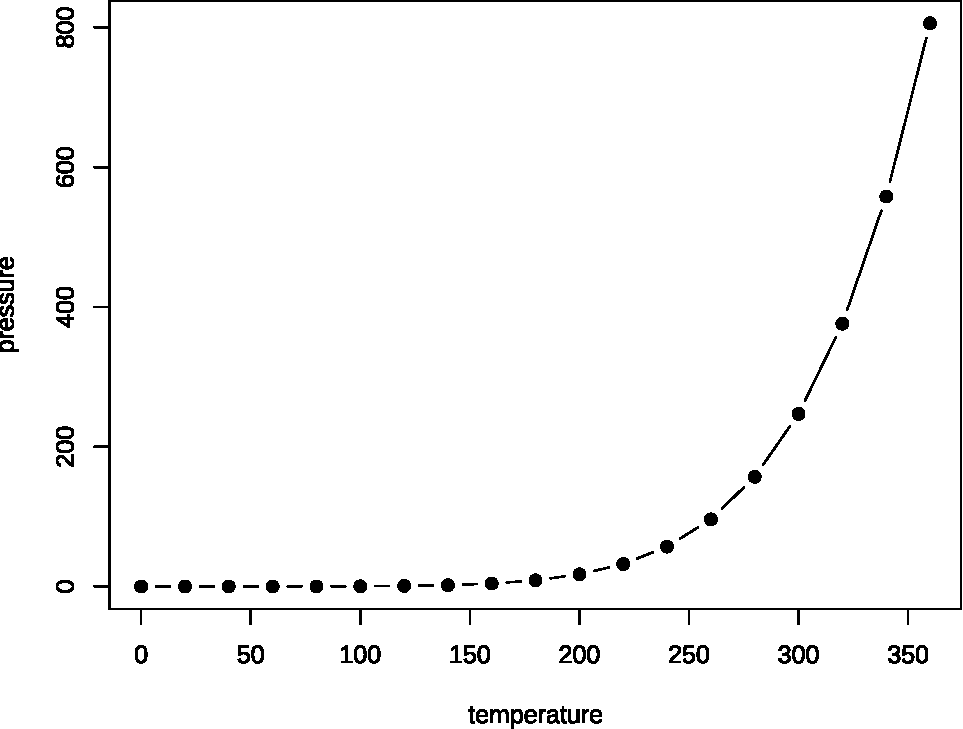
\includegraphics[width=0.8\linewidth]{90-bookdown_files/figure-latex/nice-fig-1} 

}

\caption{Here is a nice figure!}\label{fig:nice-fig}
\end{figure}

Don't miss Table \ref{tab:nice-tab}.

\begin{Shaded}
\begin{Highlighting}[]
\NormalTok{knitr}\SpecialCharTok{::}\FunctionTok{kable}\NormalTok{(}
  \FunctionTok{head}\NormalTok{(pressure, }\DecValTok{10}\NormalTok{), }\AttributeTok{caption =} \StringTok{\textquotesingle{}Here is a nice table!\textquotesingle{}}\NormalTok{,}
  \AttributeTok{booktabs =} \ConstantTok{TRUE}
\NormalTok{)}
\end{Highlighting}
\end{Shaded}

\begin{table}

\caption{\label{tab:nice-tab}Here is a nice table!}
\centering
\begin{tabular}[t]{rr}
\toprule
temperature & pressure\\
\midrule
0 & 0.0002\\
20 & 0.0012\\
40 & 0.0060\\
60 & 0.0300\\
80 & 0.0900\\
\addlinespace
100 & 0.2700\\
120 & 0.7500\\
140 & 1.8500\\
160 & 4.2000\\
180 & 8.8000\\
\bottomrule
\end{tabular}
\end{table}

\hypertarget{parts}{%
\chapter{Parts}\label{parts}}

You can add parts to organize one or more book chapters together. Parts can be inserted at the top of an .Rmd file, before the first-level chapter heading in that same file.

Add a numbered part: \texttt{\#\ (PART)\ Act\ one\ \{-\}} (followed by \texttt{\#\ A\ chapter})

Add an unnumbered part: \texttt{\#\ (PART\textbackslash{}*)\ Act\ one\ \{-\}} (followed by \texttt{\#\ A\ chapter})

Add an appendix as a special kind of un-numbered part: \texttt{\#\ (APPENDIX)\ Other\ stuff\ \{-\}} (followed by \texttt{\#\ A\ chapter}). Chapters in an appendix are prepended with letters instead of numbers.

\hypertarget{footnotes-and-citations}{%
\chapter{Footnotes and citations}\label{footnotes-and-citations}}

\hypertarget{footnotes}{%
\section{Footnotes}\label{footnotes}}

Footnotes are put inside the square brackets after a caret \texttt{\^{}{[}{]}}. Like this one \footnote{This is a footnote.}.

\hypertarget{citations}{%
\section{Citations}\label{citations}}

Reference items in your bibliography file(s) using \texttt{@key}.

For example, we are using the \textbf{bookdown} package \citep{R-bookdown} (check out the last code chunk in index.Rmd to see how this citation key was added) in this sample book, which was built on top of R Markdown and \textbf{knitr} \citep{xie2015} (this citation was added manually in an external file book.bib). Note that the \texttt{.bib} files need to be listed in the index.Rmd with the YAML \texttt{bibliography} key.

The \texttt{bs4\_book} theme makes footnotes appear inline when you click on them. In this example book, we added \texttt{csl:\ chicago-fullnote-bibliography.csl} to the \texttt{index.Rmd} YAML, and include the \texttt{.csl} file. To download a new style, we recommend: \url{https://www.zotero.org/styles/}

The RStudio Visual Markdown Editor can also make it easier to insert citations: \url{https://rstudio.github.io/visual-markdown-editing/\#/citations}

\hypertarget{blocks}{%
\chapter{Blocks}\label{blocks}}

\hypertarget{equations}{%
\section{Equations}\label{equations}}

Here is an equation.

\begin{equation} 
  f\left(k\right) = \binom{n}{k} p^k\left(1-p\right)^{n-k}
  \label{eq:binom}
\end{equation}

You may refer to using \texttt{\textbackslash{}@ref(eq:binom)}, like see Equation \eqref{eq:binom}.

\hypertarget{theorems-and-proofs}{%
\section{Theorems and proofs}\label{theorems-and-proofs}}

Labeled theorems can be referenced in text using \texttt{\textbackslash{}@ref(thm:tri)}, for example, check out this smart theorem \ref{thm:tri}.

\begin{theorem}
\protect\hypertarget{thm:tri}{}\label{thm:tri}For a right triangle, if \(c\) denotes the \emph{length} of the hypotenuse and \(a\) and \(b\) denote the lengths of the \textbf{other} two sides, we have \[a^2 + b^2 = c^2\]
\end{theorem}

Read more here \url{https://bookdown.org/yihui/bookdown/markdown-extensions-by-bookdown.html}.

\hypertarget{callout-blocks}{%
\section{Callout blocks}\label{callout-blocks}}

The \texttt{bs4\_book} theme also includes special callout blocks, like this \texttt{.rmdnote}.

You can use \textbf{markdown} inside a block.

\begin{Shaded}
\begin{Highlighting}[]
\FunctionTok{head}\NormalTok{(beaver1, }\AttributeTok{n =} \DecValTok{5}\NormalTok{)}
\CommentTok{\#\textgreater{}   day time  temp activ}
\CommentTok{\#\textgreater{} 1 346  840 36.33     0}
\CommentTok{\#\textgreater{} 2 346  850 36.34     0}
\CommentTok{\#\textgreater{} 3 346  900 36.35     0}
\CommentTok{\#\textgreater{} 4 346  910 36.42     0}
\CommentTok{\#\textgreater{} 5 346  920 36.55     0}
\end{Highlighting}
\end{Shaded}

It is up to the user to define the appearance of these blocks for LaTeX output.

You may also use: \texttt{.rmdcaution}, \texttt{.rmdimportant}, \texttt{.rmdtip}, or \texttt{.rmdwarning} as the block name.

The R Markdown Cookbook provides more help on how to use custom blocks to design your own callouts: \url{https://bookdown.org/yihui/rmarkdown-cookbook/custom-blocks.html}

\hypertarget{sharing-your-book}{%
\chapter{Sharing your book}\label{sharing-your-book}}

\hypertarget{publishing}{%
\section{Publishing}\label{publishing}}

HTML books can be published online, see: \url{https://bookdown.org/yihui/bookdown/publishing.html}

\hypertarget{pages}{%
\section{404 pages}\label{pages}}

By default, users will be directed to a 404 page if they try to access a webpage that cannot be found. If you'd like to customize your 404 page instead of using the default, you may add either a \texttt{\_404.Rmd} or \texttt{\_404.md} file to your project root and use code and/or Markdown syntax.

\hypertarget{metadata-for-sharing}{%
\section{Metadata for sharing}\label{metadata-for-sharing}}

Bookdown HTML books will provide HTML metadata for social sharing on platforms like Twitter, Facebook, and LinkedIn, using information you provide in the \texttt{index.Rmd} YAML. To setup, set the \texttt{url} for your book and the path to your \texttt{cover-image} file. Your book's \texttt{title} and \texttt{description} are also used.

This \texttt{bs4\_book} provides enhanced metadata for social sharing, so that each chapter shared will have a unique description, auto-generated based on the content.

Specify your book's source repository on GitHub as the \texttt{repo} in the \texttt{\_output.yml} file, which allows users to view each chapter's source file or suggest an edit. Read more about the features of this output format here:

\url{https://pkgs.rstudio.com/bookdown/reference/bs4_book.html}

Or use:

\begin{Shaded}
\begin{Highlighting}[]
\NormalTok{?bookdown}\SpecialCharTok{::}\NormalTok{bs4\_book}
\end{Highlighting}
\end{Shaded}


  \bibliography{book.bib,packages.bib}

\end{document}
